% Engine: XeLaTeX + biber (see build.sh). The chain below is what TeXstudio runs
% for this document; it overrides whatever "Default Compiler" is set to locally,
% and mirrors build.sh exactly (xelatex -> biber -> xelatex -> xelatex).
% !TeX TXS-program:compile = txs:///xelatex | txs:///biber | txs:///xelatex | txs:///xelatex
% !TeX TXS-program:bibliography = txs:///biber


%% bachelorarbeit.tex  --  main file
%%
%% Bachelorarbeit, Fachgruppe Soziologie, Otto-Friedrich-Universitaet Bamberg
%%
%% COMPILE (XeLaTeX -- recommended):
%%     xelatex bachelorarbeit
%%     biber   bachelorarbeit
%%     xelatex bachelorarbeit
%%     xelatex bachelorarbeit
%% or simply:   latexmk -xelatex bachelorarbeit
%% For LuaLaTeX: replace "xelatex" with "lualatex" (works identically).
%%%%%%%%%%%%%%%%%%%%%%%%%%%%%%%%%%%%%%%%%%%%%%%%%%%%%%%%%%%%%%%%%%%%%%%%%%%%%%%%%%
\documentclass[
  fontsize=12pt,     % Merkblatt 3.3: 12pt
  a4paper,
  twoside=false,     % single-sided; set true if you bind double-sided
  numbers=noenddot,
  parskip=never,     % indented paragraphs, no extra vertical gap
  chapterprefix=false,
]{scrreprt}

\usepackage[apa]{bamberg-thesis}       % all formatting rules live here

% Bibliography database -----------------------------------------------------
\addbibresource{literatur.bib}
% Force the journal-article and online examples into the bibliography so the
% template shows those formats too (remove once you write your own text):
\nocite{henz1995,dietrich2011}

% Thesis metadata (shown on the cover page) ---------------------------------
\thesistitle{Sprachkurse als Schlüssel zur Arbeitsmarktintegration von Geflüchteten? Eine Replikation und
	Erweiterung der Untersuchung von Kanas und Kosyakova (2023)}
\thesisauthor{Mehmet Emre Sümer}
\thesismatrikel{2067968}
\thesiscontact{emre\_suemer@stud.uni-bamberg.de}
\thesisfirstreviewer{Prof.\ Dr.\ Cornelia Kristen}
\thesissecondreviewer{}   % leave with {} if none, Dr.\ Zweitgutachter/in
\thesisstudiengang{Soziologie}
\thesisfaculty{Sozial- und Wirtschaftswissenschaften}
\thesisdate{\today}
\thesislogo{figures/logo-uni-bamberg}   % override the default logo path here

\begin{document}

% ---- Cover page (Deckblatt) ------------------------------------------------
\makedeckblatt

% Leerseite nach dem Deckblatt (ohne Seitenzahl), damit der Abstract beim
% beidseitigen Druck auf einer rechten Seite beginnt.
\thispagestyle{empty}
\null
\newpage

% ---- Front matter: roman page numbers --------------------------------------
\pagenumbering{roman}

% Optional preface (Vorwort). Comment out if you do not need one.
% % ---------------------------------------------------------------------------
% Vorwort (optional -- Merkblatt 3.2: Danksagung, aktueller Bezug, Motivation)
% ---------------------------------------------------------------------------
\chapter*{Vorwort}
\addcontentsline{toc}{chapter}{Vorwort}

Das Vorwort ist optional. Hier können Sie eine Danksagung unterbringen, auf
den aktuellen Bezug des Themas eingehen oder Ihre persönliche Motivation für
die Themenwahl erläutern. Fachlich-inhaltliche Ausführungen gehören dagegen
in die Einleitung, nicht in das Vorwort.

Wenn Sie kein Vorwort benötigen, entfernen Sie einfach die Zeile
\texttt{\textbackslash input\{chapters/vorwort\}} in \texttt{bachelorarbeit.tex}.


% Abstract / Kurzfassung (the English one uses correct English hyphenation).
% ---------------------------------------------------------------------------
% Abstract / Kurzfassung
% The English abstract is wrapped in an English-language block so that line
% breaking uses the correct *English* hyphenation patterns; the surrounding
% document keeps German hyphenation.
% ---------------------------------------------------------------------------
\chapter*{Abstract}
\addcontentsline{toc}{chapter}{Abstract}

\begin{otherlanguage}{english}
\noindent
This bachelor thesis replicates the study ``Greater local supply of language courses improves refugees' labor market integration'' by Kanas and Kosyakova and extends it by treating asylum status as a moderator. The analyses draw on the IAB-BAMF-SOEP Survey of Refugees, waves 2016 to 2019, combined with county-level data on the supply of integration courses; they were run through SOEPremote, the remote execution system of DIW Berlin. The replication reproduces the sample selection exactly (5,467 person-years from 2,730 persons) and confirms the central result: a one standard deviation higher course supply in the county of initial assignment is associated with a 2.98 percentage point higher probability of employment (published: 2.97).

The extension builds on Esser's action-theoretical model of language acquisition and asks whether refugees with a recognised asylum claim, who have a secure prospect of staying and unrestricted access to courses, benefit more from the local supply than refugees whose claim is pending or rejected. This is tested not only for employment but, above all, for the mechanisms of integration course participation, course completion, language certificates and German language proficiency. None of the joint interaction tests is significant; course participation comes closest (p = 0.053), with point estimates ordered as expected. The results do not support the hypothesis, but given the group sizes they do not rule out smaller differences either.
\end{otherlanguage}

\bigskip
\begin{otherlanguage}{ngerman}
\noindent\textbf{Kurzfassung.}\enspace

Diese Bachelorarbeit reproduziert die Studie „Greater local supply of language courses improves refugees' labor market integration“ von Kanas und Kosyakova und erweitert sie um den Asylstatus als Moderator. Grundlage sind die IAB-BAMF-SOEP-Befragung von Geflüchteten in den Wellen 2016 bis 2019 sowie Kreisdaten zum Angebot an Integrationskursen; die Analysen liefen über das Ferndatenverarbeitungssystem SOEPremote des DIW Berlin. Die vorliegende Arbeit reproduziert die Stichprobenselektion exakt (5.467 Personenjahre von 2.730 Personen) und bestätigt das zentrale Ergebnis: Ein um eine Standardabweichung höheres Kursangebot im Zuweisungskreis geht mit einer um 2,98 Prozentpunkte höheren Beschäftigungswahrscheinlichkeit einher (publiziert: 2,97). 

Die Erweiterung prüft auf Basis des handlungstheoretischen Spracherwerbsmodells von Esser, ob anerkannte Geflüchtete wegen sicherer Bleibeperspektive und uneingeschränktem Kurszugang stärker vom lokalen Angebot profitieren als Geflüchtete mit offenem oder abgelehntem Verfahren. Geprüft wird dies nicht nur für die Beschäftigung, sondern vor allem für die Mechanismen Integrationskursteilnahme, Integrationskursabschluss, Sprachzertifikat und Deutschkenntnisse. Kein gemeinsamer Interaktionstest ist signifikant; am nächsten kommt die Kursteilnahme (p = 0,053), bei der die Punktschätzungen in der erwarteten Reihenfolge liegen. Die Ergebnisse stützen die Hypothese nicht, schließen kleinere Unterschiede angesichts der Gruppengrößen aber auch nicht aus.

\end{otherlanguage}


% Table of contents
\tableofcontents

% Optional lists -- uncomment the ones you actually use.
\listoffigures
\listoftables
% \input{chapters/abkuerzungsverzeichnis}   % Abkuerzungsverzeichnis (optional)

% ---- Main matter: arabic page numbers, restart at 1 ------------------------
\cleardoublepage
\pagenumbering{arabic}

% Einleitung
% ---------------------------------------------------------------------------
% Einleitung (Merkblatt 3.2: Problem-/Fragestellung, Zielsetzung, Aufbau;
% Umfang max. ~15% der Seiten)
% ---------------------------------------------------------------------------
\chapter{Einleitung}
\label{cha:einleitung}

Deutschland erlebte in den Jahren 2015 und 2016 die größte Flüchtlingswelle der jüngeren Vergangenheit \parencite{brucker2016vorlaufige}. Insbesondere Kriege, Bedrohungen der Meinungsfreiheit waren einige der Gründe, die Flüchtlinge dazu veranlassten, nach Deutschland zu fliehen \parencite[4]{brucker202510}. Der 2015 ausgebrochene Bürgerkrieg in Syrien sowie die politischen und wirtschaftlichen Probleme in Ländern wie dem Irak, Afghanistan und Eritrea waren die Hauptursachen für die Flüchtlingswelle der Jahre 2015–2016 \parencites[4]{unknown}[23--24]{brucker2016vorlaufige}. Insbesondere in den Jahren 2015 und 2016 erreichte die Zahl der nach Deutschland geflüchteten Menschen ihren Höchststand. Im Jahr 2016 stellten 722.370 Menschen einen Asylantrag in Deutschland, während diese Zahl im Jahr 2017 auf 198.317 zurückging und seitdem stetig abgenommen hat \parencite[103]{fur2019migrationsbericht}. Obwohl diese Anzahl in den letzten Jahren zurückgegangen ist, hat sie seit dieser Zeit die Politik Deutschlands in den Bereichen Asyl, Migration und Integration maßgeblich beeinflusst.

Der Erwerb der deutschen Sprache ist einer der ersten Schritte im Rahmen der Integration von Geflüchteten in den Arbeitsmarkt \parencite{Bahr2019Arbeitsmarktintegration}. Angesichts der Anforderungen vieler Berufsgruppen in Deutschland, in denen für mindestens die Hälfte der Stellen Deutschkenntnisse auf dem Niveau B2 oder höher vorausgesetzt werden, sind die für Geflüchtete angebotenen Deutschkurse von entscheidender Bedeutung für eine erfolgreiche Integration in den Arbeitsmarkt \parencite{repec:iab:iabkbe:202607}. Darüber hinaus wird die Teilnahme von Migrant:innen, deren Deutschkenntnisse unter dem Niveau B2 liegen, an einem Deutschkurs als ein zu berücksichtigender Faktor angesehen. Nicht nur Unternehmen, sondern auch 52 Prozent der Arbeitssuchenden sind der Einschätzung, dass mangelnde Deutschkenntnisse bei der Arbeitssuche ein mögliches Hindernis darstellen könnten \parencite{repec:iab:iabkbe:202607}.

Die Geflüchteten verfügten anfangs nur über geringe Deutschkenntnisse. Laut Daten aus dem Jahr 2016 gaben lediglich 16 Prozent der Geflüchteten an, gut Deutsch sprechen zu können \parencite[7]{brucker2018iab}. Bei etwa der Hälfte der Geflüchteten wurde berichtet, dass sie „nicht oder eher schlecht Deutsch sprechen“ \parencite[7]{brucker2018iab}.

Bemerkenswert ist auch die anfänglich niedrige Beschäftigungsquote der Geflüchteten in Deutschland. Während im Jahr 2015 9,9 Prozent der nach Deutschland gekommenen Geflüchteten erwerbstätig waren, lag diese Quote im Jahr 2016 bei 6,2 Prozent \parencite{brucker2017arbeitsmarktintegration}. Im Laufe der Zeit war jedoch ein Anstieg der Beschäftigungsquote der Geflüchteten zu beobachten \parencite{brucker2024institutionelle}.

Nach Angaben aus dem Jahr 2016 waren lediglich 3 Prozent der Geflüchteten ohne jegliche Deutschkenntnisse erwerbstätig, während von den Geflüchteten mit geringen Deutschkenntnissen lediglich 7 Prozent erwerbstätig waren (blau) \parencite[9]{sirries2017arbeitsmarktintegration}. Im Vergleich zu anderen Möglichkeiten des Sprachenlernens profitieren Geflüchtete besonders von strukturierten Lernangeboten wie Sprachkursen \parencite{kristen2022deutschkenntnisse}. Aus diesem Grund gewinnt der Einfluss des lokalen Sprachkursangebots auf die Beschäftigung gesellschaftliche Relevanz.

Der Aufenthaltsstatus gilt als wichtiger Faktor für den Zugang von Geflüchteten zum Arbeitsmarkt. Während rechtliche Hindernisse für den Zugang von Geflüchteten mit anerkanntem Aufenthaltsstatus zum Arbeitsmarkt aufgehoben werden, bestehen für Geflüchtete, deren Aufenthaltsstatus noch nicht geklärt ist oder deren Antrag abgelehnt wurde, weiterhin bürokratische Hindernisse \parencite[128--129]{kosyakova2020role}. Darüber hinaus kann die ungewisse Aufenthaltssituation von Geflüchteten, deren Aufenthaltsstatus noch nicht feststeht oder deren Antrag abgelehnt wurde, die Entscheidungen von Arbeitgebenden beeinflussen \parencite{kosyakova2020role}. \textcite{brucker2024institutionelle} stellten fest, dass die Wahrscheinlichkeit einer Beschäftigung bei Personen mit anerkanntem Aufenthaltsstatus im Vergleich zu Personen mit abgelehntem oder ungewissem Status höher ist.

Darüber hinaus spielt der Aufenthaltsstatus eine zentrale Rolle beim Zugang zu Deutschkursen. Personen mit anerkanntem Status erhalten uneingeschränkten Zugang zu öffentlich geförderten Deutschkursen, während Personen, deren Asylantrag abgelehnt wurde, unter bestimmten Umständen im Rahmen einer Duldung das Recht auf Teilnahme an Sprachkursen erhalten \parencite[129]{kosyakova2020role}. Personen, deren Aufenthaltsstatus noch nicht geklärt ist, haben hingegen keinen uneingeschränkten Zugang zu öffentlich geförderten Sprachkursen \parencite[12]{kosyakova2020role}.

Der Aufenthaltsstatus wirkt sich sowohl auf die Beschäftigungschancen von Geflüchteten als auch auf deren Zugang zu staatlich geförderten Deutschkursen aus. Aus diesem Grund ist es aus soziologischer Sicht von Interesse, welche Gruppe von Geflüchteten im Hinblick auf die Integration durch Sprachkurse in Bezug auf die Beschäftigung am stärksten profitiert.


\textcite{Kanas:2023} untersuchten den kausalen Einfluss des Angebots an lokalen Sprachkursen in Deutschland auf die Integration von Flüchtlingen in den Arbeitsmarkt. Dabei wurde der Einfluss des Sprachkursangebots in den Landkreisen auf die Beschäftigungschancen von Geflüchteten untersucht. \textcite{Kanas:2023} stellten fest, dass die Beschäftigungschancen von Geflüchteten in den Landkreisen, in denen mehr lokale Sprachkurse angeboten werden, höher sind. Diese Arbeit zielt darauf ab, die empirischen Analysen aus dem Artikel von \textcite{Kanas:2023} zu reproduzieren, um die Ergebnisse dieser Arbeit erneut zu analysieren und um eine Erweiterung vorzunehmen. Der Beitrag dieser Arbeit besteht darin, zu untersuchen, ob Flüchtlinge, deren Aufenthaltsstatus anerkannt ist, im Hinblick auf ihren Erfolg auf dem Arbeitsmarkt stärker von dem Angebot an lokalen Sprachkursen in Deutschland profitieren. Anhand des Spracherwerbsmodells von \textcite{Esser:2006} wird in dieser Arbeit die Investition von Geflüchteten in Sprachkurse in Abhängigkeit von ihrem Aufenthaltsstatus erklärt und anschließend der Aufenthaltsstatus als Interaktionseffekt getestet. Demzufolge beantwortet diese Arbeit die folgende Forschungsfrage: „Profitieren Geflüchtete mit anerkanntem Asylantrag stärker von lokalen Sprachkursen im Hinblick auf ihren Arbeitsmarkterfolg?“


Diese Arbeit ist wie folgt aufgebaut: Der Forschungsstand gliedert sich in drei verschiedene Abschnitte. Zunächst wird der Zusammenhang zwischen dem Spracherwerb der Zielsprache und dem Erfolg auf dem Arbeitsmarkt erläutert. Anschließend werden Beiträge vorgestellt, die den Einfluss von Sprachkursen auf die Integration in den Arbeitsmarkt beleuchten. Im Hinblick auf die Erweiterung dieser Arbeit werden im letzten Abschnitt Studien vorgestellt, die sich mit dem Zusammenhang zwischen dem Aufenthaltsstatus und dem Spracherwerb im Hinblick auf die Integration in den Arbeitsmarkt befassen. Im letzten Abschnitt des Forschungsstands wird schließlich die Entwicklung von Integrationskursen und Teilnahmebescheinigungen auf Kreisebene dargestellt. „Theoretischer Rahmen“ wird in zwei Unterkapiteln behandelt. Zunächst werden die theoretischen Ansätze erläutert, mit denen Kanas und Kosyakova die Auswirkungen des lokalen Kursangebots auf die Beschäftigung erklären. Der zweite Teil des „Theoretischen Teils“ basiert auf einer theoretischen Erweiterung. Anhand des Sprachlernmodells von Esser (2006) wird theoretisch erläutert, ob sich die Auswirkungen des lokalen Kursangebots auf die Beschäftigung je nach Asylstatus unterscheiden. Im methodischen Teil werden die sowohl in „Reproduction“ als auch in „Erweiterung“ verwendeten Datensätze, die Replikationsstrategie, die Operationalisierung der Variablen sowie die Bildung der Stichprobe erläutert. Im Ergebnisteil wird die Forschungsfrage anhand der Ergebnisse von „Reproduction“ und „Erweiterung“ beantwortet.


% Hauptteil (mind. 2/3 der Arbeit) -- subdivided per Merkblatt 3.2:
%   Forschungsstand -- Theorie -- Methodik -- Ergebnisse
% ---------------------------------------------------------------------------
% Hauptteil, Teil 1: Bisheriger Forschungsstand (Merkblatt 3.2)
% Demonstriert die Zitierweise im Fliesstext (Autor-Jahr, Seite nach Doppel-
% punkt) exakt nach den Beispielen des Merkblatts (S. 7).
% ---------------------------------------------------------------------------
\chapter{Forschungsstand}
\label{cha:forschungsstand}

In diesem Abschnitt wird der aktuelle Stand der Forschungsliteratur dargestellt. Zunächst werden die Faktoren erläutert, die die Integration von Geflüchteten in den Arbeitsmarkt beeinflussen. Anschließend werden veröffentlichte Forschungsergebnisse zum Effekt von Sprachkursen auf die Arbeitsmarktintegration von Geflüchteten vorgestellt. Darauf aufbauend werden die relevanten Befunde aus Forschungsberichten zu Sprache und Arbeitsmarktintegration dargestellt. Abschließend werden bestehende Forschungslücken aufgezeigt.

\section{Sprachkenntnisse und Arbeitsmarktintegration von Geflüchteten}
\label{cha:arbeitsmarktintegration}

Im Allgemeinen besteht ein positiver Zusammenhang zwischen dem Spracherwerb der Zugewanderten in der Aufnahmelandessprache und ihren Einkommens- und Beschäftigungsaussichten \parencites{doi:10.1086/298374}{10.1111/1468-0297.t01-1-00151}. Der Spracherwerb hat deshalb für Zugewanderte einen besonderen Stellenwert auf dem Arbeitsmarkt.

Der Zusammenhang zwischen Sprachkompetenz und Arbeitsmarkterfolg gilt auch für Geflüchtete. Es liegen Belege dafür vor, dass Sprachkompetenz in einem positiven Zusammenhang mit der Beschäftigungs- und beruflichen Situation von Geflüchteten steht. Geflüchtete sind auf den Arbeitsmärkten der europäischen Länder benachteiligt, allerdings bestehen Unterschiede zwischen den verschiedenen Ländern \parencites{dumont2016refugees}{doi:10.1111/j.1747-7379.2010.00810.x}.

Der Spracherwerb ist nicht für alle Berufsgruppen von derselben Bedeutung. Je nach beruflicher Position können von Geflüchteten unterschiedliche Sprachkenntnisse verlangt werden. Der Spracherwerb bzw. das Sprachniveau kann im Kontext des Arbeitsmarktes einen unterschiedlichen Stellenwert haben \parencite{chiswick2010occupational}.

Auch für Flüchtlinge in Deutschland hat der Spracherwerb im Aufnahmeland im Hinblick auf die Integration in den Arbeitsmarkt an Bedeutung gewonnen. Bessere Sprachkenntnisse stehen auch bei Flüchtlingen in Deutschland in Zusammenhang mit der Beschäftigung \parencite{kosyakova2017large}. Darüber hinaus wurde gemäß der zweiten Erhebungswelle der IAB-BAMF-SOEP-Umfrage festgestellt, dass sowohl die Sprachkenntnisse als auch die Beschäftigungsquoten von Geflüchteten in Deutschland im Laufe der Zeit gestiegen sind \parencite{brucker2019gefluchtete}.

Der Spracherwerb ist kein statischer Vorgang, sondern entwickelt sich über einen bestimmten Zeitraum und einen bestimmten Prozess hinweg. Neben individuellen Faktoren kann auch ein strukturierter Lernprozess den Spracherwerb von Zugewanderten fördern. Dies zeigt, dass der Spracherwerb nicht nur durch den individuellen Lernprozess, sondern auch durch strukturierte Angebote wie beispielsweise Sprachkurse gefördert werden kann \parencite{Kosyakova04042022}.

\section{Empirische Evidenz zur Wirkung von Sprachkursen}
\label{cha:empirische}

Die bisherige Forschungsliteratur zeigte, dass die Teilnahme an Sprachkursen und der Erwerb der deutschen Sprache zu den wichtigsten Faktoren gehören, die den Erfolg auf dem Arbeitsmarkt fördern \parencites{brucker2019language}{lang2022employment}{marbach2025does}. Der aktuelle Stand der Forschung zeigt, dass Sprachkurse die Integration in den Arbeitsmarkt fördern. Aus den aktuellen Forschungsergebnissen geht hervor, dass Sprachkurse nicht nur das Erlernen der Sprache des Aufnahmelandes erleichtern, sondern auch dazu beitragen, dass Geflüchtete spezifische arbeitsmarktrelevante Kenntnisse und Fähigkeiten erwerben \parencite{iza:izadps:dp16091}. Sprachtraining hat somit, wie in aktuellen Studien dargelegt, einen positiven Einfluss auf die Integration in den Arbeitsmarkt. Die bisherige Forschungsliteratur zeigt, dass Sprachkurse dafür sorgen, dass Geflüchtete bessere Deutschkenntnisse erwerben, wodurch sich ihre Chancen auf eine Teilhabe am Arbeitsmarkt verbessern \parencites{lang2022employment}{marbach2025does}.

Der Forschungsstand unterscheidet, welche Deutschkurse im Hinblick auf den Arbeitsmarkt am erfolgreichsten sind. \textcite{marbach2025does} haben analysiert, dass nicht alle Sprachenkurse gleichermaßen effektiv sind. Es hat sich gezeigt, dass kurzfristige Sprachenkurse, wie beispielsweise Ad-hoc-Kurse, keinen signifikanten Einfluss auf die Beschäftigung haben \parencite{marbach2025does}. Im Vergleich zu kurzfristig angelegten Kursen haben sich langfristig angelegte und umfassendere Kurse im Hinblick auf die Arbeitsmarktintegration von Geflüchteten als effizienter erwiesen \parencite{marbach2025does}. 

\textcite{lang2022employment} analysierte die Auswirkungen von Sprachkursen auf beschäftigungslose Zugewanderte. Sie stellte fest, dass Personen, die an berufsbezogenen Sprachkursen des BAMF teilnahmen, höhere Beschäftigungsquoten aufwiesen \parencite{lang2022employment}. Berufsbezogene Kurse zielen inhaltlich nicht nur auf den Erwerb der deutschen Sprache ab, sondern sind eine Kursart, die auch die Förderung arbeitsmarktspezifischer Sprachkompetenzen wie berufliche Kommunikation und Deutsch am Arbeitsplatz zum Ziel hat \parencite{lang2022employment}. Berufssprachkurse verbessern nicht nur die Deutschkenntnisse der Teilnehmenden, sondern tragen auch zur Erweiterung ihrer arbeitsmarktrelevanten Kenntnisse bei und wirken sich somit positiv auf ihre Beteiligung am deutschen Arbeitsmarkt aus. Dieses Ergebnis ist insbesondere in der Anfangsphase stärker ausgeprägt und bei Frauen im Vergleich zu Männern deutlicher zu erkennen \parencite{lang2022employment}. Zusammenfassend lässt sich festhalten, dass nicht jeder Sprachkurs die Integration von Geflüchteten in den Arbeitsmarkt in gleichem Maße beeinflusst; insbesondere Sprachkurse, die arbeitsmarktrelevante Kompetenzen fördern, haben sich positiv auf Beschäftigung und Einkommen ausgewirkt \parencite{lang2022employment}

\section{Aufenthaltsstatus und Arbeitsmarktintegration}
\label{cha:aufenthaltsstatus}

Im Vergleich zu anderen Zugewanderten sind Geflüchtete beim Spracherwerb und bei der Beschäftigungssuche mit gewissen Nachteilen konfrontiert \parencites{10.3389/fpos.2022.977764}{10.1093/epolic/eix008}. Einer der zentralen Faktoren für den Erfolg von Geflüchteten auf dem Arbeitsmarkt ist das Zielsprachenerlernen \parencite{Kosyakova04042022}. Aus diesem Grund bieten viele Aufnahmeländer, wie beispielsweise Deutschland, Sprach- und Integrationskurse für Geflüchtete an \parencite{kristen2021destination}.

\textcite{Kanas:2023} haben den kausalen Zusammenhang zwischen lokalen Sprachkursen in Deutschland und den Beschäftigungsaussichten von Geflüchteten untersucht. Die Analyse ergab, dass ein hohes Angebot an Sprachkursen in dem Landkreis, in den Geflüchtete zugewiesen werden, ihre Beschäftigungsaussichten verbessert. Der Zusammenhang zwischen dem Angebot an lokalen Sprachkursen und der Beschäftigung wurde zudem anhand von Mechanismen wie dem Abschluss eines Sprachkurses, der Häufigkeit des Kontakts zu Deutschen und der Sprachkompetenz untersucht.

Der Zusammenhang zwischen dem Aufenthaltsstatus von Geflüchteten und dem Arbeitsmarkt wurde in der Forschungsliteratur intensiv untersucht. Bisherige Untersuchungen zeigen, dass der ungewisse Aufenthaltsstatus von Geflüchteten und die lange Dauer des Asylverfahrens zu Verzögerungen bei der Integration der Geflüchteten in den Arbeitsmarkt führten \parencites{article}{doi:10.1126/sciadv.1600432}.

Unabhängig vom Ergebnis des Aufenthaltsstatus haben bisherige Untersuchungen gezeigt, dass eine schnelle Klärung des Aufenthaltsstatus dazu beitragen kann, dass Geflüchtete schneller mit einem Sprachkurs beginnen und eine Beschäftigung aufnehmen können \parencite{kosyakova2020role}. In diesem Zusammenhang wurde darauf hingewiesen, dass nicht nur der Aufenthaltsstatus, sondern auch ein schneller Ablauf des Asylverfahrens eine wichtige Rolle spielt. 

\textcite{10.1257/aer.89.2.186} erläutern, dass Migrant:innen entsprechend ihren eigenen Zielen in Humankapital investieren und dabei eine Kosten-Nutzen-Abwägung entsprechend ihren Zielen vornehmen. Dem zentralen Ergebnis zufolge führt ein sicherer Aufenthaltsstatus bei Migrant:innen dazu, dass sie einen höheren Nutzen aus ihren zielgerichteten Investitionen erwarten. Das heißt, aus der Perspektive der Bleibeperspektive kann ein sicherer Aufenthaltsstatus dazu führen, dass Migrant:innen einen größeren Nutzen aus den getätigten Investitionen erwarten \parencite{10.1257/aer.89.2.186}.

\textcite{repec:iab:iabdpa:202031} wenden diesen Gedanken in Form eines Choice-Experiments auf Deutschland an. Zu den zentralen Schlussfolgerungen gehört, dass die Gewissheit über die Zukunft der Geflüchteten in Deutschland sie dazu motivieren könnte, in Humankapital wie Sprache und Bildung zu investieren. Außerdem wird darauf hingewiesen, dass ein sicherer Aufenthaltsstatus dazu motiviert, in Humankapital wie Sprache und Ausbildung zu investieren \parencite{repec:iab:iabdpa:202031}.

Neben dem rechtlichen Aufenthaltsstatus kann auch die subjektive Bleibeabsicht der Zugewanderten im Zielland die Integration beeinflussen. \textcite{doi:10.1177/09500170261425857} unterteilten die Geflüchteten in drei verschiedene Gruppen: diejenigen, die dauerhaft bleiben möchten, diejenigen, die vorübergehend bleiben möchten, und diejenigen, deren Bleibeabsicht unklar ist. Das wichtigste Ergebnis ist die Beobachtung, dass Geflüchtete, die eine vorübergehende Bleibeperspektive im Aufnahmeland haben, im Vergleich zu denen, die dauerhaft bleiben möchten, geringere Sprachkenntnisse aufweisen. Außerdem wird eine unklare Bleibeperspektive im Aufnahmeland als nachteilig für den Spracherwerb der Geflüchteten erklärt \parencite{doi:10.1177/09500170261425857}.

Insgesamt zeigte die bisherige Forschung, dass Statusunsicherheit und längere Asylverfahren den Integrationsprozess von Flüchtlingen verlangsamen können \parencites{article}{doi:10.1126/sciadv.1600432}. Zudem wurde beobachtet, dass Flüchtlinge, die über einen sicheren Aufenthaltsstatus verfügen, durch Investitionen in Humankapital – wie Sprache und Bildung – größere Gewinne erzielen können \parencite{10.1257/aer.89.2.186}. Schließlich steht auch die subjektive Bleibeabsicht in Zusammenhang mit der Integration in den Arbeitsmarkt \parencite{doi:10.1177/09500170261425857}.



\section{Der deutsche Kontext}
\label{cha:deutsche_kontext}


\subsection{Das deutsche Integrations- und Sprachkurssystem}
\label{sec:deu-integ}

Ein Großteil der Fluchtbewegung der letzten Jahren fand zwischen 2015 und 2019 statt, und im Jahr 2016 stellten 722.370 Personen in Deutschland einen Asylantrag \parencite[13]{BAMF2020}. Deutschland ist daher in den letzten Jahren im Zusammenhang mit der Fluchtbewegung zu einem Zielland geworden \parencite{https://doi.org/10.1111/1467-9361.00008}. Dieser Anstieg der Fluchtbewegung seit 2015 hat auch zu politischen Veränderungen hinsichtlich der integrationspolitischen Maßnahmen in Deutschland geführt. 

Die Inhalte der vom BAMF durchgeführten Integrationskurse umfassten sowohl die Zielsprache als auch kulturelle Komponenten. Integrationskurse in Deutschland werden vom Staat organisiert und gelten als wichtiges Instrument für die Integration von Geflüchteten in Deutschland. Die Hauptaufgabe der Integrationskurse besteht darin, Deutschkurse für Migranten in Deutschland, vor allem für Geflüchtete, anzubieten. Das Ziel der Sprachkurse ist das Sprachniveau GER B1 \parencite{council2001common}. Neben der sprachlichen Förderung zielen sie darauf ab, grundlegende Kenntnisse über das Rechtssystem, die Geschichte und die Kultur Deutschlands zu vermitteln \parencite{Rother_2014}. Der allgemeine Kurs umfasst 600 Stunden Sprachunterricht, während der Orientierungskurs aus 100 Stunden besteht. Das übergeordnete Ziel besteht darin, die soziale und wirtschaftliche Integration von Geflüchteten in Deutschland zu fördern \parencite{Rother_2014}.

Personen, die in Deutschland einen Asylantrag gestellt haben, erhalten Berechtigungsscheine bzw. eine Teilnahmeberechtigung für die Teilnahme an Integrationskursen. Anfangs wurde das Teilnahmerecht nur Personen mit anerkanntem Asylantrag gewährt, jedoch wurde das Teilnahmerecht im Jahr 2015 erweitert \parencite{kosyakova2020role}. Auch Personen, bei denen die Wahrscheinlichkeit einer Anerkennung ihres Asylantrags hoch ist, sowie Personen, deren Asylantrag noch geprüft wird, erhielten das Recht zur Teilnahme an den Kursen. Auch in Ausnahmefällen erhielten Asylbewerber mit Duldungsstatus das Recht auf Teilnahme \parencite{kosyakova2020role}.

Zwischen 2014 und 2016 stieg die Zahl der Integrationskurse auf das Doppelte. Die Zahl der im Jahr 2016 begonnenen Integrationskurse erreichte 20.000 \parencite{grote2018changing}. Neben den vom Staat organisierten Kursen gab es weitere Programme, die von Bundesländern, Kommunen, zivilgesellschaftlichen Organisationen und Hilfsorganisationen angeboten wurden \parencites{kosyakova2020role}{brucker2020has}. Das Besondere an den Integrationskursen ist, dass sie neben dem Sprachunterricht eine umfassendere Integrationsförderung bieten. Obwohl die Zahl der Sprachkurse deutschlandweit gestiegen ist, blieb die Teilnehmerzahl hinter den Erwartungen zurück. Zwischen 2013 und 2016 nahm nur ein Drittel der Personen, die in Deutschland einen Asylantrag gestellt hatten, an einem Integrationskurs teil. Im Jahr 2017 stieg dieser Anteil jedoch an, sodass 55 Prozent der Betroffenen an einem Integrationskurs teilnahmen.


\subsection{Regionale Variation des Kursangebots}
\label{sec:erg-angebot}

Die Entwicklung der Integrationskurse in Deutschland zwischen den Jahren 2015 und 2016 ist in \ref{fig:kursangebot}  dargestellt. Panel A veranschaulicht die prozentuale Entwicklung der Integrationskurse auf Landkreisebene. Panel B zeigt die prozentuale Entwicklung der Erteilung von Teilnahmeberechtigungen für Sprachkurse für Geflüchtete zwischen 2015 und 2016. Abbildung~\ref{fig:kursangebot} ermöglicht einen Vergleich zwischen der Entwicklung der Integrationskurse und der Entwicklung der Berechtigungsbescheinigungen für Sprachkurse im Zeitraum von 2015 bis 2016.


\begin{figure}[htbp]
	\centering
	% Der Vektor-Master liegt als figures/fig01_both_panels.svg vor. XeLaTeX kann
	% SVG nicht direkt einbinden (dafuer waeren das svg-Paket, Inkscape und
	% --shell-escape noetig, was build.sh bewusst nicht verwendet); eingebunden
	% wird daher die 300-dpi-PNG-Fassung derselben Grafik.
	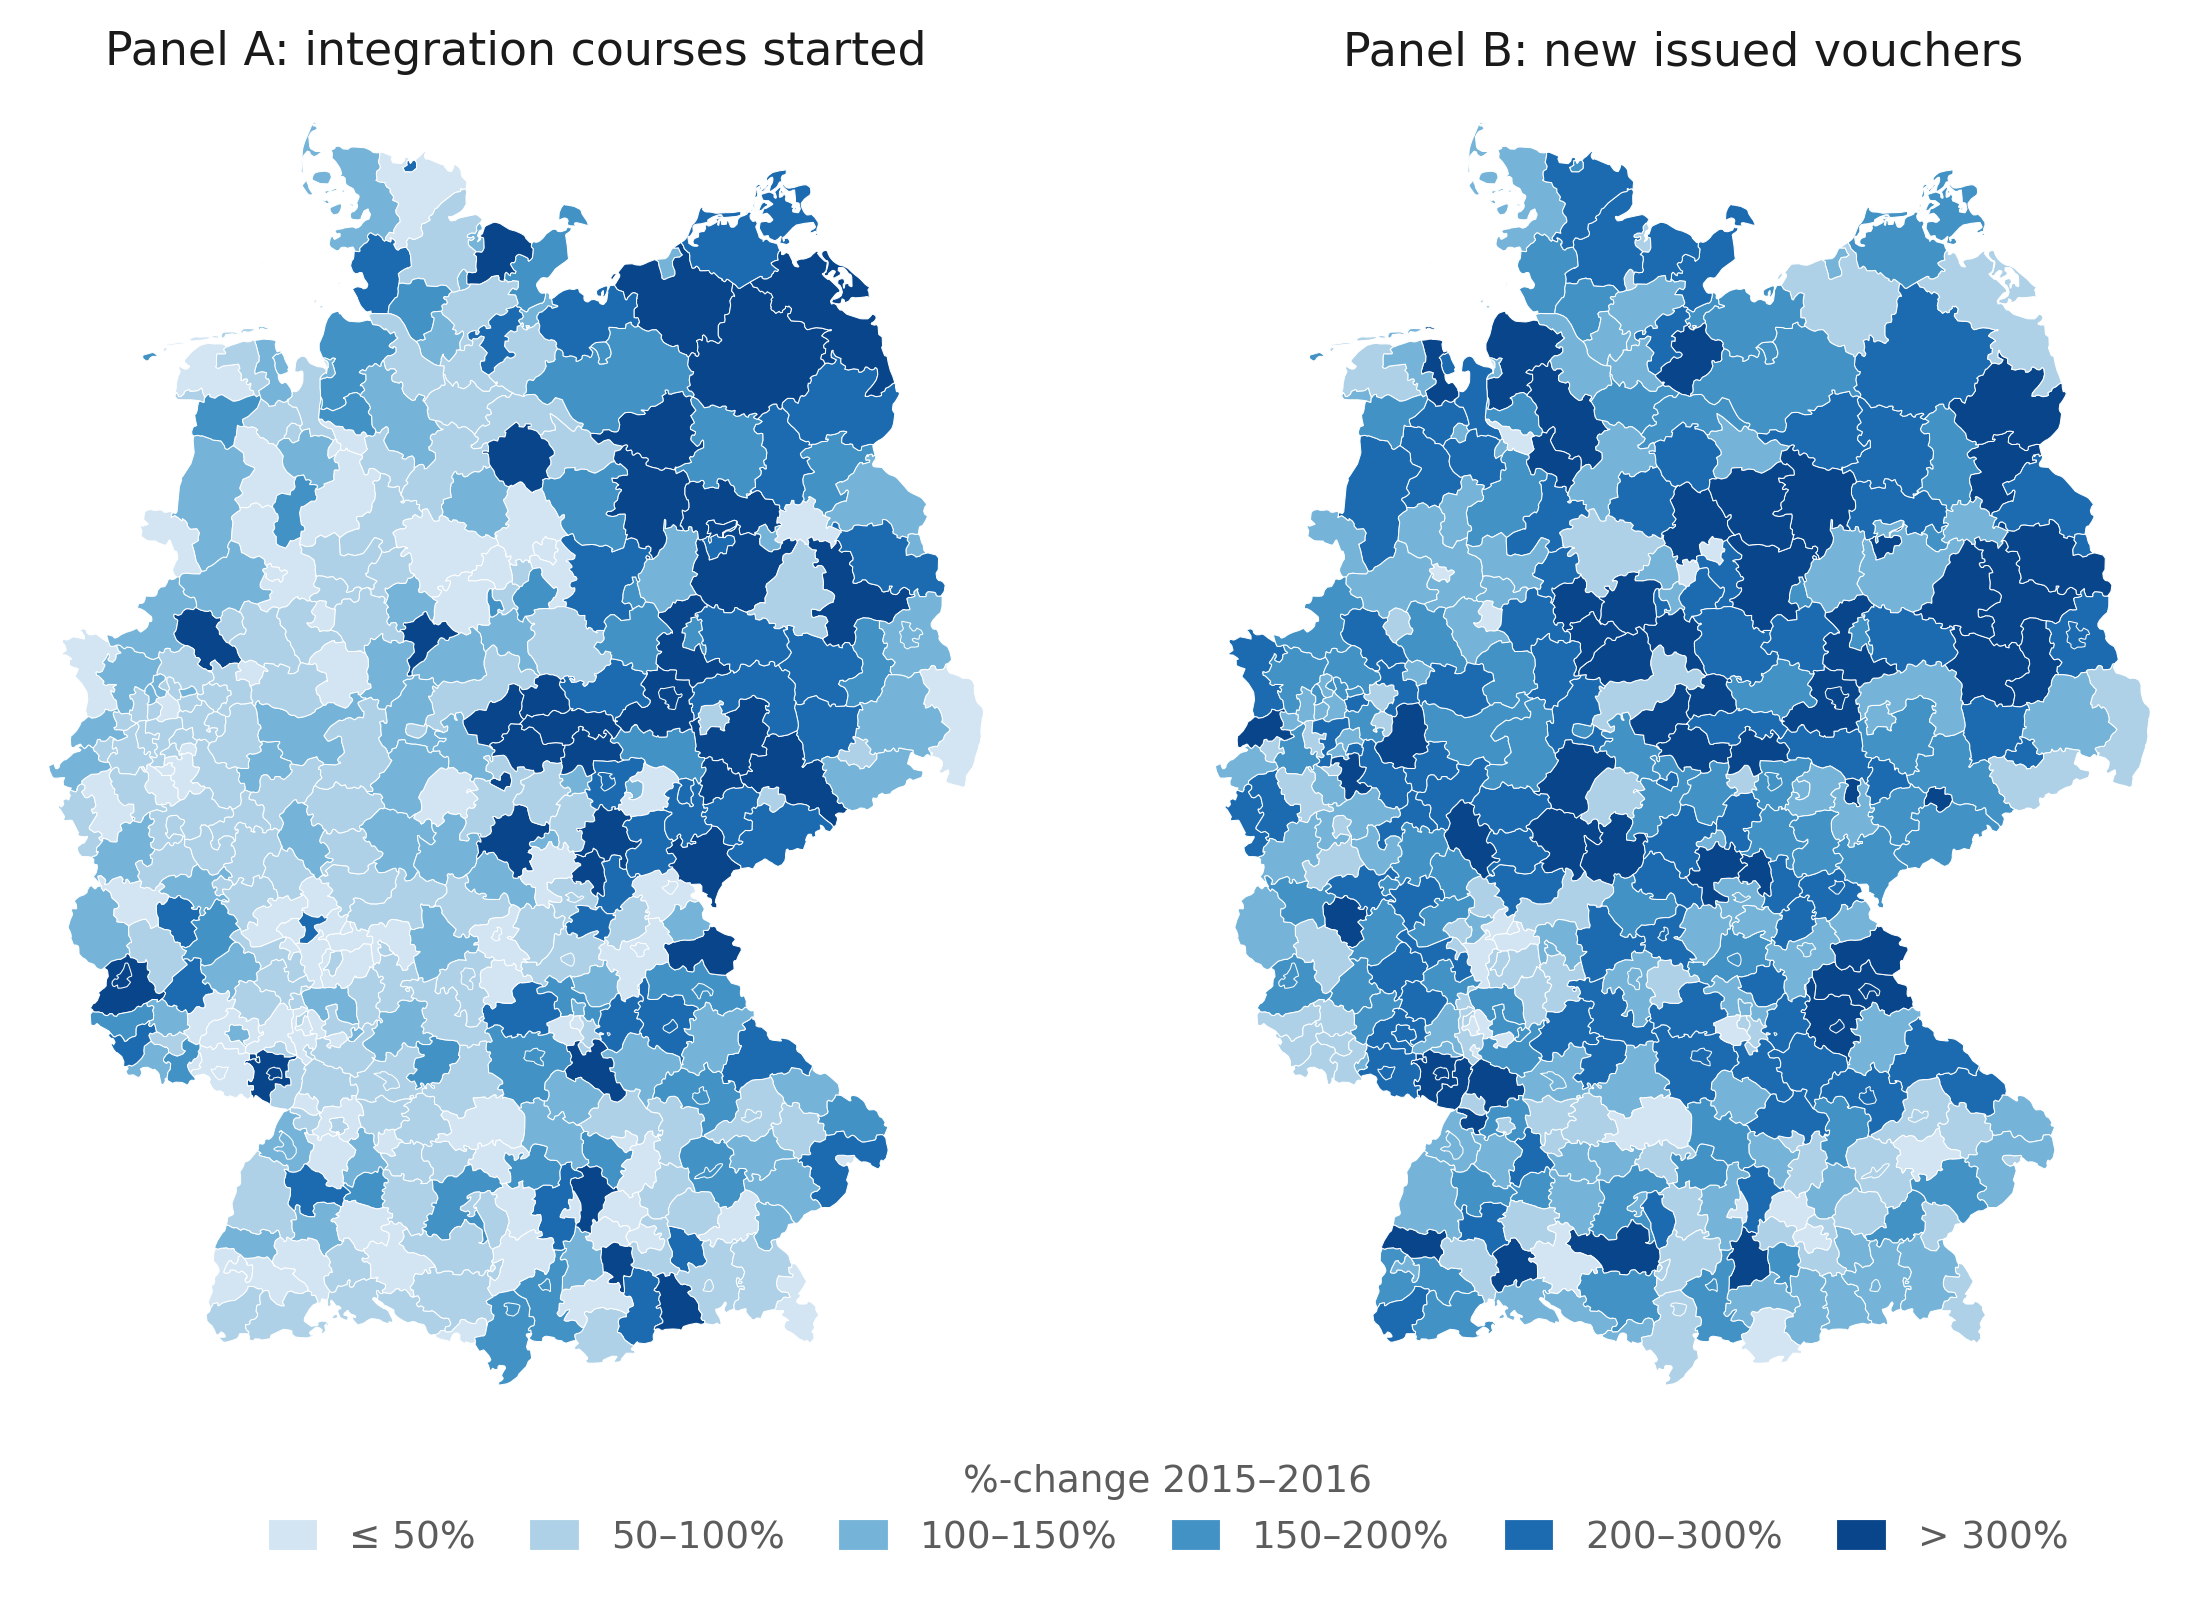
\includegraphics[width=\textwidth]{figures/fig01_both_panels.png}
	\caption[Ver\"anderung des Angebots an Integrationskursen 2015--2016 nach
	Kreisen]{Ver\"anderung des Angebots an Integrationskursen zwischen 2015 und
		2016 nach Kreisen. Panel~A: begonnene Integrationskurse; Panel~B: neu
		ausgestellte Berechtigungsscheine. Eigene Darstellung auf Basis der
		BAMF-Kursstatistik; Kreisgrenzen nach VG2500 (BKG). Entspricht Abbildung~1
		in \textcite{Kanas:2023}.}
	\label{fig:kursangebot}
\end{figure}

Sowohl Panel A als auch Panel B zeigen, dass zwischen den Kreisen deutliche Unterschiede zu beobachten sind. In einigen Kreisen steigt der Anteil der Integrationskurse, während der Anstieg in anderen Kreisen geringer ausfällt. Ähnliches gilt auch für die Berechtigungsbescheinigungen, die zum Kursbesuch für Geflüchtete ausgestellt werden. Während der Anstieg bei den ausgegebenen Berechtigungsbescheinigungen in einigen Regionen gering ist, ist er in anderen Regionen sehr deutlich. Aus diesem Grund ist die Entwicklung der Integrationskurse in Deutschland nicht in gleichem Maße vorangeschritten.

Die reproduzierte \ref{fig:kursangebot} zeigt uns, dass die Entwicklung der Integrationskurse in einem Kreis und die Zunahme der ausgestellten Berechtigungsnachweise nicht unbedingt im gleichen Maße verlaufen. Während die Angebot an Integrationskursen in einem Kreis zunimmt, kann es sein, dass bei ausgegebenen Berechtigungsnachweisen kein sichtbarer Anstieg zu beobachten ist. \ref{fig:kursangebot} zeigt auch, dass das genaue Gegenteil der Fall sein kann. Damit wird veranschaulicht, dass regionale Unterschiede zwischen Angebot und Nachfrage bei Integrationskursen auftreten können.

Beim Vergleich verschiedener Kreise in Deutschland lassen sich auffällige Unterschiede feststellen. Sowohl bei den Integrationskursen als auch bei der Entwicklung der Berechtigungsnachweise gibt es Unterschiede auf Kreisebene. Dies lässt sich so interpretieren, dass es auf Kreisebene zu regionalen Unterschieden beim Zugang zu Integrationskursen führen kann.

\textcite{Kanas:2023} zeigen, dass sich die Zahl der Berechtigungsnachweise in 165 Kreisen um mehr als das Doppelte erhöht hat. Die Zahl der Integrationskurse hat sich jedoch im Vergleich zum Vorjahr in weniger als der Hälfte der 165 Kreise verdoppelt. Dies lässt sich damit erklären, dass die Nachfrage nach Integrationskursen in einem Kreis nicht im gleichen Maße zugenommen hat wie die Entwicklung der Integrationskurse.

Insgesamt bestehen regionale Unterschiede hinsichtlich der Entwicklung der Integrationskurse und der an Geflüchtete ausgestellten Teilnahmebescheinigungen. Beispielsweise ist nicht zu beobachten, dass das Angebot an Integrationskursen in einem Kreis im gleichen Maße zunimmt mit der Anzahl der ausgestellten Teilnahmebescheinigungen.

\subsection{Arbeitsmarktzugang von Geflüchteten}
\label{sec:arb-zugang}

Der Zugang von Geflüchteten zum Arbeitsmarkt wird durch rechtliche Verfahren zentral geregelt. Die Arbeitserlaubnisse für Geflüchtete unterscheiden sich von anderen Migranten und können teilweise restriktiv sein. Das Herkunftsland und die aufenthaltsrechtliche Situation der Geflüchteten spielen in diesem Zusammenhang eine wesentliche Rolle \parencite{kosyakova2020role}.

Während Personen, deren Asylantrag noch nicht abgeschlossen ist, in den ersten drei Monaten keine Arbeitserlaubnis erhalten, können diese Personen danach unter bestimmten rechtlichen Voraussetzungen eine Arbeitserlaubnis erhalten. Personen, deren Asylverfahren noch nicht abgeschlossen ist, haben aus diesem Grund nur eingeschränkten Zugang zum Arbeitsmarkt \parencite{kosyakova2020role} .

Personen, deren Asylantrag anerkannt wurde, verfügen über unterschiedliche Schutzstatus. Diese Schutzstatus lassen sich wie folgt auflisten: Asylberechtigte, Personen mit subsidiärem Schutzstatus und Personen mit nationalem Abschiebungsverbot. Für Personen mit diesen Schutzstatus gelten keine Einschränkungen hinsichtlich der Beschäftigung \parencite{muller2016unterstutzungsmassnahmen}.

Der Arbeitsmarktzugang von Personen mit Duldungsstatus ist in Deutschland ebenfalls eingeschränkt; eine Arbeitserlaubnis wird nur unter bestimmten gesetzlichen Voraussetzungen erteilt \parencites{kosyakova2020role}{stache2024auswirkungen}. Zusammenfassend lässt sich feststellen, dass für Personen, deren Asylantrag genehmigt wurde, keine Hindernisse beim Zugang zum Arbeitsmarkt bestehen. Für Personen, deren Asylantrag abgelehnt wurde oder deren Asylantrag noch in Bearbeitung ist, gelten jedoch bestimmte rechtliche Einschränkungen.

Ähnliche Einschränkungen gelten auch für Integrationskurse. Mit Ausnahme von Personen, für die ein nationales Abschiebungsverbot gilt, haben alle Flüchtlinge mit dem Status „aufnahmeberchtigt“ das uneingeschränkte Recht auf Teilnahme an Integrationskursen \parencite{stache2024auswirkungen} . Für Personen mit dem Status „Duldung“ besteht das Recht auf Teilnahme an Integrationskursen jedoch nur unter bestimmten rechtlichen Einschränkungen. Es wurde berichtet, dass Personen mit Duldung, die über gute Bleibeperspektiven verfügen, an Integrationskursen teilnehmen dürfen \parencite{kosyakova2020role}.

\subsection{Räumliche Verteilung und Wohnsitzauflage}
\label{sec:raum-vert-wohn}

\textcite{Kanas:2023} erläuterten, wie der erste Wohnort von Geflüchteten in Deutschland bei ihrer Ankunft zugewiesen wurde. Die Zuweisung des ersten Wohnorts von Geflüchteten ist sowohl für die Bildung der Stichprobe als auch für die Beschreibung der unabhängigen Variablen „Angebot an Kursen auf Kreisebene“ von großer Bedeutung.

Die Verteilung der Flüchtlinge innerhalb Deutschlands erfolgt nicht ausschließlich auf der Grundlage individueller Entscheidungen; zusätzlich gibt es einen staatlich gesteuerten Verteilungsmechanismus, der die Verteilung der Geflüchteten innerhalb Deutschlands übernimmt. Die Verteilung erfolgt zunächst zwischen den Bundesländern, anschließend findet die Verteilung innerhalb der einzelnen Bundesländer statt. Der anfängliche Wohnort der Geflüchteten wird somit nicht ausschließlich nach deren eigenen Entscheidungen bestimmt \parencite{geis2016fluchtlinge}.

\textcite{Kanas:2023} beschäftigten sich mit den Faktoren, die die Verteilung von Geflüchteten in Deutschland beeinflussen. Die vorhandene Unterkunftskapazität, die städtische Struktur und die Arbeitslosenquote auf lokaler Ebene gehörten zu den entscheidenden Faktoren für die Verteilung der Geflüchteten innerhalb Deutschlands \parencites {entorf2019refugees}{geis2016fluchtlinge}.


Nach der erstmaligen Zuweisung von Geflüchteten in eine Region ist die Bewegungsfreiheit eingeschränkt. Während des laufenden Asylverfahrens oder für Personen, deren Asylantrag abgelehnt wurde, gelten Aufenthaltsbeschränkungen \parencite{haberstroh2020migration}. Im Jahr 2016 gab es jedoch Änderungen. Im Rahmen dieser Regelung galten auch für Flüchtlinge, deren Asylantrag angenommen wurde, für einen bestimmten Zeitraum Bewegungsbeschränkungen \parencite[108]{haberstroh2020migration}. Insgesamt galten somit auch für Personen, deren Asylantrag anerkannt wurde, für einen bestimmten Zeitraum Aufenthaltsbeschränkungen. 


Da die Personen den gewünschten Kreis nicht selbst wählen dürfen, nimmt das „Residential Sorting“ ab \parencite{Kanas:2023}.Die Beschränkung des Wechsels von einem Kreis in einen anderen ermöglicht eine zuverlässigere Untersuchung des Kursangebots. Gäbe es eine freie Wohnortwahl, könnte eine Person aus persönlichen Gründen in einen anderen Kreis umziehen; dies könnte die Untersuchung erschweren, ob der Zusammenhang zwischen Kursen und Beschäftigung tatsächlich auf die Kurse zurückzuführen ist.






% Hinweise zur Zitierweise (Merkblatt 3.4):
%   \autocite{key}          -> (Autor Jahr)
%   \autocite[229]{key}     -> (Autor Jahr: 229)          [Doppelpunkt konfiguriert]
%   \autocite[vgl.][229]{k} -> (vgl. Autor Jahr: 229)
%   \autocite{k1,k2}        -> (Autor1 Jahr1; Autor2 Jahr2)
%   \textcite{key}          -> Autor (Jahr)  im Satzfluss
% Vermeiden Sie eine bloße Aneinanderreihung von Zitaten und beziehen Sie die
% Literatur systematisch und kritisch auf Ihre Fragestellung.

% ---------------------------------------------------------------------------
% Hauptteil, Teil 2: Theorie (Theoriedarstellung, Ausgangsannahmen, Hypothesen)
% ---------------------------------------------------------------------------
\chapter{Theoretischer Rahmen}
\label{cha:theorie}

Der theoretische Teil der Arbeit erläutert zunächst, anhand welcher Theorien in dem Artikel von Kanas und Kosyakova die Auswirkungen der lokalen Sprachkurse auf die Arbeitsmarktintegration beschrieben werden. Es wird erläutert, wie die Hypothesen des replizierten Artikels anhand der theoretischen Ansätze abgeleitet und wie versucht wurde, sie zu erklären. Anschließend wird im Abschnitt „Theoretische Weiterentwicklung“ erläutert, inwiefern dieser reproduzierte Artikel theoretisch erweitert bzw. ergänzt wird.

In dem reproduzierten Artikel wird anhand von vier verschiedenen theoretischen Ansätzen erläutert, warum ein höheres lokales Kursangebot die Integration von Geflüchteten in den Arbeitsmarkt beeinflusst. Die erste dieser Theorien ist die von Becker entwickelte Humankapitaltheorie. Die Humankapitaltheorie geht davon aus, dass Sprachkurse dank besserer Sprachkenntnisse und spezifischer Informationen über den Arbeitsmarkt des Aufnahmelandes die Produktivität steigern. Die Signaling-Theorie hingegen ist eine weitere Theorie, die erklärt, dass die durch Sprachkurse erworbenen Zertifikate bei fehlenden Informationen die Lernfähigkeit einer Person belegen. Die Grundannahme von Collins’ Social-Closure- bzw. Credentialing-Theorie ist, dass Sprachzertifikate eine Schlüsselrolle dabei spielen, Barrieren beim Zugang zum Arbeitsmarkt zu beseitigen. 

Abschließend wird die Theorie des Sozialkapitals – eine Theorie, die versucht, die Integration in den Arbeitsmarkt anhand von aufgebauten Netzwerken und sozialen Beziehungen zu erklären – zur Erläuterung der Forschungsfrage herangezogen. Als theoretische Weiterentwicklung wird die Komplementarität des Humankapitals nach Chiswick als Erweiterung des theoretischen Konzepts erläutert.

\section{Humankapitaltheorie}
\label{cha:human}

Die Humankapitaltheorie ist eine ökonomische Theorie, die auf der Grundidee basiert, dass das Wissen und die Fähigkeiten von Menschen in der Zukunft einen ökonomischen Ertrag erbringen können \parencite{becker1964human}. Der grundlegende Mechanismus dieser Theorie erläutert, dass Humankapital die Produktivität steigern und somit dem Individuum einen ökonomischen Ertrag bringen kann.

Das Wissen und die Fähigkeiten der Menschen werden aus ökonomischer Sicht betrachtet. Der Begriff „Humankapital“ beinhaltet das von Menschen erworbene Wissen und die Fähigkeiten. Becker erläutert, dass Humankapital ebenso wie physisches Kapital die Produktivität des Individuums steigert. Demnach wird Humankapital als das Wissen und die Fähigkeiten definiert, die die Produktivität der Menschen steigern \parencite[7--10]{becker1964human}.

Der Begriff der Investition spielt bei der Entstehung von Humankapital eine wichtige Rolle. Eine Investition bezeichnet Tätigkeiten, die Menschen gegenwärtig ausüben und die in der Zukunft einen wirtschaftlichen Nutzen bringen können. Gemäß der Humankapitaltheorie ist eine Investition mit Kosten verbunden. Die Kosten der Investition stehen in einem Zusammenhang mit dem künftigen Ertrag. Das Individuum trägt die Kosten in der Gegenwart, jedoch wird davon ausgegangen, dass diese Investition dem Individuum in der Zukunft einen ökonomischen Nutzen bringen kann. Insgesamt steigern Investitionen in das Humankapital das Humankapital des Individuums, indem sie dessen Wissen und Fähigkeiten fördern. Es wird angenommen, dass mit steigendem Humankapital die Produktivität des Individuums zunehmen kann und dies in der Zukunft zu höheren ökonomischen Erträgen führen kann \parencite[7--10]{becker1964human}.

Gemäß Beckers Theorie des Humankapitals kann der Spracherwerb als eine Form von Humankapital verstanden werden. Die Teilnahme an Sprachkursen lässt sich als eine Investition der Geflüchteten in ihr Humankapital verstehen. Es ist anzunehmen, dass Geflüchtete durch die Teilnahme an Sprachkursen in Zukunft über bessere Deutschkenntnisse verfügen werden. Die Teilnahme der Geflüchteten an lokalen Sprachkursen in Deutschland kann mit Kosten wie Zeit, Geld und Aufwand verbunden sein. Durch die Teilnahme an Sprachkursen erworbene Deutschkenntnisse können die Produktivität von Geflüchteten steigern und ihre Beschäftigung auf dem Arbeitsmarkt fördern \parencite{becker1964human}.

Eine ähnliche Verbindung zwischen Sprachkursen, Humankapital und Arbeitsmarktintegration wird auch von \textcite{Kanas:2023} hergestellt. Das lokale Angebot an Sprachkursen kann dazu beitragen, dass Migrant:innen ihre aufnahmelandspezifischen Kenntnisse und Fähigkeiten weiterentwickeln können. Durch die Teilnahme an Sprachkursen können Kenntnisse und Fähigkeiten erworben werden, die die Produktivität auf dem Arbeitsmarkt steigern können, beispielsweise bei Vorstellungsgesprächen oder bei der Kommunikation mit Arbeitskolleg:innen, wodurch Geflüchtete im Beschäftigungskontext von einem Nutzen profitieren könnten.

\section{Signaling-Theorie}
\label{cha:Signal}

Ein weiterer theoretischer Ansatz, der die Auswirkungen der Förderung lokaler Deutschkurse auf die Beschäftigung zu erklären versucht, ist Signaling-Theorie~\parencite{Spence1973}. Spences Signaling-Theorie ist ein theoretisches Modell, das das Problem erklärt, wie Arbeitgebende die Produktivität und das Leistungspotenzial von Arbeitssuchenden einschätzen, wenn sie darüber nur unvollständige Informationen besitzen \parencite[55--56]{Spence1973}.

Arbeitgebende hingegen können die Produktivität und das Potenzial des Arbeitssuchenden vor der Einstellung nicht vollständig einschätzen. Aus diesem Grund basiert dieser theoretische Ansatz auf der Informationsasymmetrie zwischen Arbeitgebenden und Arbeitssuchenden. In Spences Modell verfügen Arbeitgebende nur über unvollständige Informationen über die Produktivitätsfähigkeiten des Arbeitssuchenden. Für Arbeitgebende stehen daher beobachtbare Merkmale im Vordergrund. Laut Spence lassen sich beobachtbare Merkmale aus zwei verschiedenen Perspektiven erklären. Sie werden in zwei Kategorien unterteilt: Indizes und Signale. Indizes bezeichnen Merkmale, die der Person nicht zu kontrollieren und nicht zu verändern sind, während Signale als Merkmale definiert werden, die der Person zu kontrollieren und zu verändern stehen. Diese Unterscheidung bildet die Grundlage für Spences Definition des Begriffs „Signal“ \parencite[357--358]{Spence1973}.

Der Erwerb eines Sprachzertifikats wird hingegen als potenzielles Signal angesehen. Eine Person, die ein Sprachzertifikat erwirbt, kann Arbeitgebenden durch dieses Zertifikat die Möglichkeit geben, Rückschlüsse auf ihre Trainingsfähigkeit und Motivation zu ziehen. Dem Modell zufolge dient der Erwerb eines Sprachzertifikats Arbeitgebenden als Hinweis auf die Fähigkeiten oder das Potenzial der Person. Auf diese Weise können Arbeitgebende Rückschlüsse auf die Motivation, Produktivität und das Potenzial der Person ziehen \parencite[357--359]{Spence1973}.

Nach Spences Modell ist das Signalisieren mit Kosten verbunden. Diese Kosten müssen nicht unbedingt monetärer Natur sein. Es handelt sich auch um nicht-monetäre Kosten wie Aufwand, Mühe und Zeit. Während der Erwerb eines Zertifikats für produktive Personen mit geringeren Kosten verbunden ist, sind für Personen mit geringer Produktivität höhere Kosten erforderlich. Auf diese Weise können Arbeitgebende Rückschlüsse auf die nicht direkt beobachtbaren Eigenschaften der Person ziehen \parencite[359]{Spence1973}.

Auch wenn die durch Sprachkurse erworbenen Zertifikate die Leistungsfähigkeit von Arbeitssuchenden nicht unmittelbar steigern, ermöglichen sie es Arbeitgebenden, Rückschlüsse auf die Fähigkeiten des Arbeitssuchenden auf dem Arbeitsmarkt zu ziehen. Nach dem Signalmodell von Spence können Zertifikate als Signale für produktivitätsrelevante Eigenschaften wie Fähigkeiten, Motivation und Engagement fungieren und dadurch die Beschäftigungswahrscheinlichkeit von Arbeitssuchenden erhöhen \parencite[355--356]{Spence1973}.

\textcite{Kanas:2023} haben die Signaling-Theorie als einen möglichen theoretischen Ansatz zur Erklärung der Auswirkungen des Angebots an Sprachkursen auf die Integration in den Arbeitsmarkt herangezogen. Dieser Ansatz basiert auf der Annahme, dass Arbeitgebende über unvollständige Informationen über die Bewerbenden verfügen und daher auf Signale zurückgreifen. Auf Grundlage dieses theoretischen Ansatzes lassen sich, wie auch bei Kanas und Kosyakova, die Beschäftigungschancen von Geflüchteten in Deutschland erklären. In dem Artikel wird darauf hingewiesen, dass es für Arbeitgebende schwierig sein kann, die in den Herkunftsländern erworbenen Bildungsabschlüsse und ähnliche Zeugnisse von Geflüchteten zu bewerten. Daher stellen die im Aufnahmeland erworbenen Zertifikate bzw. Teilnahmebescheinigungen von Deutschkursen für Arbeitgebende besser beobachtbare und bewertbare Informationen dar. In Deutschland erworbene Sprachzertifikate liefern nicht nur ein verlässliches Signal hinsichtlich der Sprachkompetenzen von Geflüchteten, sondern ermöglichen es Arbeitgebenden auch, anhand dieser Zertifikate Rückschlüsse auf die Motivation und die Trainierbarkeit der Geflüchteten auf dem deutschen Arbeitsmarkt zu ziehen. Durch dieses Signal können Arbeitgebende eine positive Einschätzung des Arbeitssuchenden vornehmen, sodass dessen Beschäftigungschancen steigen könnten.

\section{Soziale Schließung und Credentialing}
\label{cha:Soziale Schließung}

„Credentialing“ ist ein theoretischer Ansatz, der von \textcite{collins1979credential} entwickelt wurde und auf der Annahme beruht, dass Zertifikate/Dokumente als Auslesemechanismus für eine bestimmte Arbeitsstelle dienen können. Nach \textcite{collins1979credential}’ Ansatz können Instrumente wie Ausbildung oder Sprachkurse zwar die Kenntnisse und Fähigkeiten des Individuums verbessern, im Arbeitsmarkt können Zertifikate/Dokumente jedoch eine Art Vorbedingung darstellen. Die Teilnahme bzw. Nichtteilnahme an einem Integrationskurs oder der Erwerb eines Zertifikats steht im Einklang mit Collins’ theoretischem Ansatz. Aus diesem Grund wird in dieser Arbeit der mögliche Einfluss der von Geflüchteten im Rahmen des Integrationskurses erworbenen Zeugnisse und Zertifikate auf die Beschäftigung anhand von Collins’ Credentialing-Theorie erläutert.

Die Credentialing-Theorie wird im Zusammenhang mit sozialer Schließung erläutert. Der Zugang zu bestimmten Stellen ist möglicherweise nicht für alle offen. Als Voraussetzung können Arbeitgebende bestimmte Ausbildungsnachweise, Sprachzertifikate und ähnliche Unterlagen verlangen. Diese Voraussetzung kann Personen, die nicht über die erforderlichen Zertifikate bzw. Unterlagen verfügen, von der Stellenbewerbung ausschließen; daher steht sie im Zusammenhang mit sozialer Schließung. Credentials bieten einer Gruppe Vorteile hinsichtlich der Mobilität, während die Mobilität der anderen Gruppe dadurch eingeschränkt wird \parencite[31--34]{collins1979credential}.



\section{Die Perspektive des Sozialkapitals}
\label{cha:sozialkapital}

\textcite{Kanas:2023} haben auf der Grundlage verschiedener Studien die Auswirkungen von Sprachkursen auf die Integration in den Arbeitsmarkt aus der Perspektive der Sozialkapitaltheorie erklärt. Das grundlegende theoretische Argument stützt sich darauf, dass durch Sprachkurse ein intensiverer Kontakt zwischen Flüchtlingen und der lokalen Bevölkerung hergestellt werden kann und dass dadurch die Integration der Geflüchteten in den Arbeitsmarkt verstärkt werden kann.

\textcite{doi:10.1111/imre.12130} haben versucht, die Frage zu beantworten, ob die Teilnahme an Sprachkursen durch türkische und marokkanische Zugewanderte langfristig Auswirkungen auf den Kontakt mit der lokalen Bevölkerung hat. Das zentrale Ergebnis der Studie zeigt, dass Sprachkurse nicht nur einen positiven Einfluss auf die Sprachkenntnisse haben, sondern auch einen positiven Zusammenhang mit dem Kontakt der Zugewanderten zur einheimischen Bevölkerung aufweisen. Aus diesem Grund können Sprachkurse Zugewanderten die Möglichkeit bieten, soziale Kontakte zur lokalen Bevölkerung aufzubauen.

\textcite{schuller2011integrationspanel} untersuchen die Ergebnisse der vom BAMF durchgeführten Integrationskurse. Die Studie befasst sich mit der Frage, inwieweit Integrationskurse für Zugewanderte nachhaltig und erfolgreich sind. In diesem Zusammenhang wurden Faktoren wie die Verbesserung der Deutschkenntnisse und die Häufigkeit der Kontakte zu Deutschen berücksichtigt und analysiert. \textcite{schuller2011integrationspanel} haben gezeigt, dass die Häufigkeit der Kontakte zu Deutschen zu Beginn des Kurses bei 3,4 lag und am Ende des Kurses bei 3,6 \parencite[233]{schuller2011integrationspanel}. Die Studie kam zu dem Ergebnis, dass die Teilnahme an Integrationskursen es zuwandernden Personen nicht nur ermöglicht, ihre Deutschkenntnisse zu verbessern, sondern auch die Häufigkeit der Kontakte zu Deutschen zu steigern.

\textcite{doi:10.1111/j.1747-7379.2010.00810.x} erläutern den Zusammenhang zwischen dem Kontakt zur lokalen Bevölkerung und der Integration in den Arbeitsmarkt. \textcite{doi:10.1111/j.1747-7379.2010.00810.x} haben festgestellt, dass der Kontakt von Geflüchteten in den Niederlanden zur lokalen Bevölkerung positiv mit deren Beschäftigungschancen zusammenhängt. Der Begriff „Bridging ties“ bezeichnet die sozialen Netzwerke, die Geflüchtete mit Menschen außerhalb ihrer eigenen Herkunftsgruppe aufbauen. Es wurde festgestellt, dass Geflüchtete mit einem höheren Anteil an „Bridging ties“ einen besseren beruflichen Status aufweisen.

Sprachkurse dienen nicht nur dem Spracherwerb, sondern können auch den Kontakt der Geflüchteten zur lokalen Bevölkerung stärken, wodurch diese einen besseren beruflichen Status erlangen können, wie dargelegt wurde. \textcite{Kanas:2023} haben im Rahmen dieser Untersuchungen versucht, zu erläutern, dass lokale Sprachkurse die Beschäftigungschancen von Geflüchteten durch die Schaffung von Kontaktmöglichkeiten zur lokalen Bevölkerung verbessern können. Da Sprachkurse den Geflüchteten die Möglichkeit bieten, die für den Kontakt mit der lokalen Bevölkerung erforderlichen Fähigkeiten zu erwerben, sind \textcite{Kanas:2023} zu der Vermutung gelangt, dass dies mit der Integration der Geflüchteten in den Arbeitsmarkt in Zusammenhang stehen könnte.


\section{Theoretische Erweiterung: Das handlungstheoretische Modell des Spracherwerbs (nach Esser)}
\label{cha:Erweiterung}

Die theoretische Erweiterung wird anhand des von \textcite{Esser:2006} entwickelten „Handlungstheoretischen Modells des Spracherwerbs“ erklärt. Das handlungstheoretische Modell des Spracherwerbs basiert auf der Vorstellung, dass das Erlernen einer Sprache eine Investition darstellt. Das Modell geht davon aus, dass Menschen für den Erwerb einer Sprache finanzielle Mittel, Zeit und persönlichen Aufwand einsetzen oder auf andere nutzenbringende Aktivitäten verzichten können. Esser weist darauf hin, dass das Erlernen einer Zweitsprache dem Individuum dadurch einen Nutzen bringen kann. Insbesondere bei Erwachsenen wird das Sprachenlernen als Investition betrachtet. Esser setzt den Spracherwerb mit bestimmten Aspekten des Humankapitals in Verbindung. Sprachkenntnisse stellen eine Eigenschaft oder Fähigkeit dar. Diese Fähigkeit lässt sich auf produktive Weise verwenden. Auf dem Arbeitsmarkt können diese Fähigkeiten beispielsweise produktiv genutzt werden. Außerdem erfordert der Spracherwerb Ressourcen. Aus diesem Grund beschreibt Esser das Erlernen einer Sprache als Investition, und darauf basiert der Ausgangspunkt seines Modells zum Spracherwerb \parencite[59--63]{Esser:2006}.

\textcite{Esser:2006} erklärt das Modell des Spracherwerbs anhand von vier verschiedenen Faktoren. Diese sind: Motivation, Zugang, Effizienz und Kosten. Der erste Baustein von Essers Investitionsmodell ist die Motivation. Die Motivation stellt den Unterschied zwischen dem Nutzen der neuen Sprache und dem aktuellen Nutzen der Muttersprache des Individuums dar. Im Modell wird der erwartete Nutzen des Erlernens der Zielsprache als U(L2) definiert, während der Nutzen der bestehenden Muttersprache des Individuums als U(L1) definiert wird. Die Motivation ist keine einzelne Zahl, sondern repräsentiert diesen Unterschied. Ein weiterer wichtiger Faktor für das Investitionsmodell sind die Strukturen des Zugangs bzw. der Zugangsmöglichkeiten. Der Kontakt des Menschen mit der Zielsprache im Alltag kann in diesem Zusammenhang beispielsweise als „Exposure“ gewertet werden. Auch Sprachkurse können in diesem Zusammenhang einen strukturierten Zugang zur Zielsprache ermöglichen. Ein weiterer Faktor ist die Effizienz. Diese wird definiert als der Anteil, in dem sprachlicher Input tatsächlich in Lernen umgewandelt wird. Als Determinanten der Effizienz werden beispielsweise das Einreisealter, die Intelligenz und die kulturelle Distanz angeführt. Schließlich fallen Kosten für den Lernprozess an. Zu den Kosten des Spracherwerbs zählen insbesondere Zeitkosten und andere Aufwendungen. Insbesondere beim gesteuerten Spracherwerb, etwa durch die Teilnahme an einem Sprachkurs, können dabei materielle Kosten und ein zusätzlicher zeitlicher Aufwand entstehen \parencite[82--89]{Esser:2006}. Das Verhältnis dieser vier Faktoren untereinander wird in der Gleichung~\eqref{eq:spracherwerb} des Investitionsmodells von \textcite{Esser:2006} dargestellt.

\begin{equation}
	U(L2) - U(L1) > C(L2) / p(exp) p(eff)
	\label{eq:spracherwerb}
\end{equation}

Die Differenz zwischen dem erwarteten Nutzen des Erwerbs einer Zweitsprache (L2) und dem Nutzen der bereits vorhandenen Sprache spiegelt die Motivation wider. C(L2) steht für die Kosten des Erwerbs der Sprache des Aufnahmelandes, p(exp) für die Möglichkeiten des Zugangs zur Zielsprache und p(eff) für die Effizienz des Spracherwerbs. Insgesamt erklärt Gleichung/Formel~\eqref{eq:spracherwerb}, dass bei geringerer Effizienz und eingeschränktem Zugang zum Spracherwerb ein höherer Motivationswert erforderlich ist.


\begin{figure}[htbp]
	\centering
	\resizebox{\textwidth}{!}{% <- keeps it inside the text block
		

	\begin{tikzpicture}[
	x=12cm, y=8cm,                    % <- overall size of the plot
	>={Latex[length=3mm,width=2mm]},
	font=\normalsize,
	case/.style={circle, fill, inner sep=2.4pt},
	tick/.style={circle, fill, inner sep=1.4pt}
	]
	
	%% ---------- adjustable parameters -------------------------------
	\def\Cm{0.22}      % cost constant of the low-cost curve  C(L2)_-
	\def\Cp{0.52}      % cost constant of the high-cost curve C(L2)_+
	\def\Mp{0.80}      % M_+  high motivation
	\def\Mz{0.44}      % M_0  medium motivation
	\def\Mm{0.14}      % M_-  low motivation
	\def\px{0.15}      % p    low  access x efficiency
	\def\pplus{0.82}   % p_+  high access x efficiency
	\def\ymax{1.30}    % top of the vertical axis
	
	%% ---------- axes -------------------------------------------------
	\draw[->] (0,0) -- (0,\ymax);
	\draw[->] (0,0) -- (1.16,0);
	
	\node[anchor=south west, align=left, inner sep=1pt] at (0.005,\ymax)
	{U(L2)-U(L1)\\ Motivation};
	\node[anchor=north west] at (1.085,-0.015) {$p(\mathrm{L2})$};
	\node[anchor=north]      at (0.45,-0.06)   {Zugang $\cdot$ Effizienz};
	
	%% ---------- tick marks -------------------------------------------
	\foreach \y/\lab in {\Mp/{$M_+$}, \Mz/{$M_0$}, \Mm/{$M_-$}}{
		\node[tick] at (0,\y) {};
		\node[anchor=east] at (-0.014,\y) {\lab};
	}
	\node[tick] at (\px,0)    {};
	\node[tick] at (\pplus,0) {};
	\node[anchor=north] at (0,-0.015)      {$0$};
	\node[anchor=north] at (\px,-0.015)    {$p$};
	\node[anchor=north] at (\pplus,-0.015) {$p_+$};
	\node[anchor=north] at (1,-0.015)      {$1$};
	
	%% ---------- the two cost curves  C/p ------------------------------
	% high-cost curve (dashed)
	\draw[dashed, dash pattern=on 8pt off 6pt, samples=400, smooth,
	domain={\Cp/\ymax}:1] plot (\x, {\Cp/\x});
	% low-cost curve (solid)
	\draw[samples=400, smooth,
	domain={\Cm/\ymax}:1] plot (\x, {\Cm/\x});
	
	\node at (0.50,{\Cp/0.50-0.13}) {$C_+/p$};
	\node at (0.50,{\Cm/0.50-0.09}) {$C_-/p$};
	
	%% ---------- right-hand end points, dotted vertical at p = 1 -------
	\draw[dotted, thick] (1,0) -- (1,\ymax);
	\node[tick] at (1,\Cp) {};
	\node[tick] at (1,\Cm) {};
	\node[anchor=west] at (1.02,\Cp) {$C(\mathrm{L2})_+$};
	\node[anchor=west] at (1.02,\Cm) {$C(\mathrm{L2})_-$};
	\node[anchor=west] at (1.02,{(\Cp+\Cm)/2}) {Kosten};
	
	%% ---------- region labels -----------------------------------------
	\node at (0.66,1.14) {Spracherwerb};
	\node[align=center] at (0.40,0.115) {kein\\ Spracherwerb};
	
	%% ---------- the six cases ------------------------------------------
	\foreach \x/\y/\n in {0.175/\Mp/1, 0.175/\Mz/2, 0.175/\Mm/3,
		\pplus/0.90/4, \pplus/\Mz/5, \pplus/\Mm/6}{
		\node[case] at (\x,\y) {};
		\node[anchor=east] at ({\x-0.022},\y) {\n};
	}
	
	%% ---------- outer frame ---------------------------------------------
	\draw ($(current bounding box.south west)+(-0.025,-0.02)$)
	rectangle
	($(current bounding box.north east)+(0.025,0.02)$);
	
\end{tikzpicture}


	

%
	}
	\caption[Motivation, Zugang, Effizienz und Kosten beim Spracherwerb]{%
		Das Zusammenspiel von Motivation, Zugang, Effizienz und Kosten beim
		(Zweit-)Spracherwerb. Eigene Darstellung in Anlehnung an
		% TODO: Seitenzahl bei Esser 2006 noch verifizieren
		\textcite[76]{Esser:2006}.}
	\label{fig:spracherwerb}
\end{figure}


Abbildung~\ref{fig:spracherwerb} veranschaulicht, wie die Entscheidung zum Sprachenlernen von Zugewanderten zustande kommt. Bei geringem Zugang zur Zielsprache und verminderter Effizienz wird ein höherer U(L2)-Bedarf erläutert, damit das Erlernen der Zweitsprache stattfinden kann. In ähnlicher Weise wird dargelegt, dass bei steigenden Kosten möglicherweise eine höhere Motivation erforderlich ist, um die Entscheidung zum Erlernen der Zielsprache zu treffen. Die Punkte in Abbildung~\ref{fig:spracherwerb} zeigen Situationen, in denen Spracherwerb je nach Kombination aus Motivation, Zugang und Effizienz möglich ist oder nicht. Außerdem erklären die verschiedenen Kurven die Kosten und deren Höhe. Demnach muss die Motivation für den Spracherwerb steigen, wenn die Kosten steigen.

\textcite{Esser:2006} verbindet die Motivation zum Erlernen einer Zweitsprache (L2) mit der Zeitperspektive sowie der Rückkehr- bzw. Bleibeperspektive. Im Zusammenhang mit der Zeitperspektive nach der Migration wurden Faktoren wie die Verwendbarkeit der Sprache und biografische Ziele als Faktoren genannt, die mit der Motivation zum Erlernen der Zielsprache in Zusammenhang stehen \parencite[82]{Esser:2006}. Es ist zu erwarten, dass die Motivation zum Erlernen einer Zweitsprache (L2) im Falle einer temporären Migration und einer Rückkehrorientierung abnehmen könnte.

Nach \textcite{Esser:2006} Modell des Spracherwerbs kann ein Sprachkurs den Zugang verbessern und die Effizienz steigern. Der Nutzen, den eine Person durch das Erlernen einer Sprache erzielt, kann jedoch auch mit der Motivation zusammenhängen. Aus diesem Grund ist zu erwarten, dass Flüchtlinge mit einem sicheren Aufenthaltsstatus hinsichtlich ihrer Bleibeperspektive tendenziell eine höhere Motivation aufweisen, in die Zielsprache (L2) zu investieren. Demgegenüber ist davon auszugehen, dass die Motivation zum Erlernen der Zielsprache bei Geflüchteten, deren Asylantrag abgelehnt wurde oder deren Asylantragsverfahren noch nicht abgeschlossen ist, tendenziell geringer ist. Insgesamt wird angenommen, dass sich die Geflüchteten je nach ihrem Aufenthaltsstatus unterscheiden lassen, welche Gruppe stärker vom lokalen Sprachkursangebot profitiert.

\textcite{Esser:2006} weist darauf hin, dass die Sprachkenntnisse von Geflüchteten auf dem Arbeitsmarkt verwendet werden können. Demnach kann davon ausgegangen werden, dass die Motivation zum Sprachenlernen bei Geflüchteten, deren Asylantrag anerkannt wurde, aufgrund ihrer Bleibeperspektiven tendenziell zunehmen könnte und dass sie stärker von lokalen Sprachkursen profitieren könnten. Infolgedessen wird davon ausgegangen, dass die erlernte Zielsprache auf dem Arbeitsmarkt produktiv verwendet werden kann \parencite[68--70]{Esser:2006}.

% ---------------------------------------------------------------------------
% Hauptteil, Teil 3: Methodik (Erhebungs-, Auswahl- und Analysemethoden)
% ---------------------------------------------------------------------------
\chapter{Methodik}
\label{cha:methodik}

In diesem Kapitel wird der methodische Aufbau der vorliegenden Replikations- und Erweiterungsstudie erläutert. Zunächst werden das Forschungsdesign sowie die Replikations- bzw. Erweiterungsstrategie erläutert. Nach der Vorstellung der verwendeten Datenbasis und der Stichprobe werden anschließend die Bildung der analytischen Stichprobe sowie die Operationalisierung der für die empirische Analyse relevanten Variablen erläutert. Abschließend wird die empirische Analysemethode dargestellt, mit der sowohl die Ergebnisse der Originalstudie repliziert als auch die im Rahmen dieser Arbeit vorgenommene Erweiterung empirisch untersucht werden.

\section{Forschungsdesign und Replikationsstrategie}
\label{cha:replikationsstrategie}

\textcite{Kanas:2023} verwenden in ihrer Studie ein natürliches Experiment. Ziel ist es, den kausalen Einfluss der Verfügbarkeit von lokalen Sprachkursen für Geflüchtete in Deutschland auf deren Integration in den Arbeitsmarkt zu untersuchen.

Das natürliche Experiment basiert auf dem Identifikationsproblem. Es wird betont, dass die Tatsache, dass die Geflüchteten ihren Wohnort (Bundesland oder Kreis) selbst wählen können, zu einem Problem der Wohnortauswahl führen könnte. Motivierte und lernwillige Geflüchtete könnten sich in Bundesländern oder Kreisen niederlassen, in denen mehr Deutschkurse angeboten werden. Dies würde den Zusammenhang zwischen dem Angebot an Deutschkursen und der Integration der Geflüchteten in den Arbeitsmarkt möglicherweise nicht korrekt widerspiegeln.

Aufgrund der „Initial Allocation Policy“ (EASY) wird der erste Wohnort der Geflüchteten vom Staat zugewiesen, sodass sie keinen eigenen Wohnort wählen dürfen. Durch die „Wohnsitzauflage“ kann der Wohnort der Geflüchteten vom Staat zugewiesen werden, wodurch ihre Mobilität hinsichtlich der Wahl eines Wohnorts in anderen Regionen eingeschränkt wird.

Die „Treatment“-Gruppe wird nicht als Teilnahme von Geflüchteten an Sprachkursen definiert. \textcite{Kanas:2023} definieren Treatment als das lokale Angebot an Integrationskursen im Landkreis, in dem die Person wohnt. Die Autorinnen beschreiben dies als Intention-to-Treat-Design. 

Die Replikationsstrategie dieser Arbeit basiert darauf, das grundlegende empirische Design der Originalstudie zu reproduzieren. In der Originalstudie untersuchten \textcite{Kanas:2023} im Rahmen eines natürlichen Experiments den kausalen Einfluss der in Deutschland für Geflüchtete verfügbaren Integrationskurse auf die Integration der Geflüchteten in den deutschen Arbeitsmarkt. Unter Berücksichtigung des empirischen Vorgehens der ursprünglichen Studie wird versucht zu testen, ob sich die Ergebnisse reproduzieren lassen.

Das Forschungsdesign, die analytische Stichprobe, die Operationalisierung der Variablen und die Regressionsstrategie des Originalartikels werden weiterhin beibehalten. Der Originalartikel untersucht die heterogenen Effekte des Angebots an Sprachkursen auf die Integration von Geflüchteten in den Arbeitsmarkt. Der Beitrag zum Originalartikel besteht darin, zu untersuchen, ob sich die Wirkung des Angebots an Sprachkursen auf die Beschäftigung je nach Asylstatus unterscheidet. Der konkrete Beitrag dieser Erweiterung ist die Untersuchung, welche Gruppe von Geflüchteten am stärksten vom Angebot an Sprachkursen profitiert.

\section{Datenbasis und Stichprobe}
\label{cha:datenbasis}

Die vorliegende Arbeit sowie die ursprüngliche Studie von \textcite{Kanas:2023} basieren auf dem Datensatz „IAB-BAMF-SOEP Survey of Refugees“ als Hauptdatensatz \parencite{iab_bamf_soep_2021}. Dieser Datensatz umfasst Asylsuchende und Flüchtlinge in Deutschland. Die erste Welle der IAB-BAMF-SOEP-Flüchtlingsbefragung wurde 2016 durchgeführt und umfasste Geflüchtete und Asylsuchende, die seit 2013 nach Deutschland gekommen waren. Die Stichprobe wurde auf Grundlage des Ausländerzentralregisters (AZR) gezogen. Der Datensatz wird vom IAB, dem BAMF-FZ und dem SOEP/DIW Berlin als repräsentative Längsschnittbefragung von Haushalten durchgeführt. Durch die Längsschnittbefragung ist es möglich, dieselben Personen über verschiedene Erhebungswellen hinweg zu untersuchen. Diese Längsschnittbefragung bietet die Möglichkeit, die Situation von Geflüchteten auf dem Arbeitsmarkt im Zeitverlauf zu untersuchen. Im Originalartikel wurden die vier Erhebungswellen aus den Jahren 2016 bis 2019 gepoolt. Die daraus resultierende Ausgangsstichprobe umfasst 18.342 Beobachtungen von insgesamt 8.321 Personen.

Der Datensatz „BAMF-Integrationskurs-Geschäftsstatistik“ wird als Zusatzdatensatz verwendet \parencite{BAMF2020}. Dieser Datensatz enthält Informationen über die Entwicklung der Integrationskurse auf Kreisebene sowie über die Anzahl der an Geflüchtete ausgegebenen Teilnahmescheine. Die DESTATIS-Daten wurden als Hauptquelle für die Kontrollvariablen auf Kreisebene verwendet. Die Variablen Bevölkerungsdichte, Arbeitslosenquote, Ausländeranteil und CDU/CSU-Stimmenanteil wurden anhand des DESTATIS-Datensatzes erstellt \parencite{destatis_2021e,destatis_2021d,destatis_2021c,destatis_2021b,destatis_2021a}. Somit stammt der Großteil der kontextbezogenen Kontrollvariablen auf Kreisebene aus den amtlichen Statistiken von DESTATIS, während für die Variable „Angst vor Zuwanderung“ die SOEP-Daten verwendet wurden.


\section{Bildung der analytischen Stichprobe}
\label{cha:bildung}

Die zu Beginn verwendete Stichprobe besteht aus 8.321 Personen und 18.342 Personenbeobachtungen. Kanas und Kosyakova planten, Flüchtlinge, die einer restriktiven Wohnsitzauflage unterliegen, in ihre Untersuchung einzubeziehen. Der Grund dafür ist, dass ein Umzug von Flüchtlingen aus dem Landkreis, dem sie zunächst zugewiesen wurden, in eine andere von ihnen gewünschte Region zu einem Problem des residential sorting/self selection führen kann. Es wird angenommen, dass die Einbeziehung ausschließlich von Flüchtlingen mit Wohnsitzauflage in die Stichprobe dieses Problem reduziert. Daher wurde angegeben, dass 2.713 Personen / 7.279 Personenjahre ausgeschlossen wurden.

%==============================================================================%
% tab01_sample_selection.tex
%
% Purpose : Tabelle 1 der Replikation - Stichprobenselektion von der Ausgangs-
%           zur Analysestichprobe. Entspricht Table 1 in Kanas & Kosyakova,
%           S. 15 (Bib-Key: Kanas:2023). Zweite (optionale) Tabelle: direkter
%           Abgleich publizierte Werte vs. Replikation.
% Source  : SOEPremote job 244563, src/stata/remote/clean_sample.do, 2026-08-13
%           Rohlisting: build/logs/src_stata_remote_clean_sample.do.eml
%           Transkript: results/comparisons/tab01_sample_funnel.md
% Needs   : booktabs, tabularx  (beide bereits in bachelorarbeit.sty geladen)
% Usage   : %==============================================================================%
% tab01_sample_selection.tex
%
% Purpose : Tabelle 1 der Replikation - Stichprobenselektion von der Ausgangs-
%           zur Analysestichprobe. Entspricht Table 1 in Kanas & Kosyakova,
%           S. 15 (Bib-Key: Kanas:2023). Zweite (optionale) Tabelle: direkter
%           Abgleich publizierte Werte vs. Replikation.
% Source  : SOEPremote job 244563, src/stata/remote/clean_sample.do, 2026-08-13
%           Rohlisting: build/logs/src_stata_remote_clean_sample.do.eml
%           Transkript: results/comparisons/tab01_sample_funnel.md
% Needs   : booktabs, tabularx  (beide bereits in bachelorarbeit.sty geladen)
% Usage   : \input{tables/tab01_sample_selection}
% Author  : Emre Suemer, 2026-08-13
%
% Zahlformat: deutsch (Punkt als Tausendertrennzeichen), passend zur
% ngerman-Sprachumgebung der Arbeit. Fuer englische Formatierung die Punkte
% in den Zahlen durch Kommata ersetzen.
%
% Zitation: verweist auf den Bib-Eintrag Kanas:2023 in literatur.bib.
%==============================================================================%

% Kriterienspalte: linksbuendig (ohne \raggedright streckt tabularx die schmale
% Spalte der Vergleichstabelle zu unschoenen Wortabstaenden) und mit haengendem
% Einzug, damit Folgezeilen langer Kriterien unter dem Text und nicht am linken
% Rand beginnen.
\makeatletter
\@ifundefined{NC@rewrite@Z}{%
  \newcolumntype{Z}{>{\raggedright\arraybackslash\hangindent=1.9em\hangafter=1}X}%
}{}
\makeatother

\begin{table}[htbp]
  \centering
  \caption{Stichprobenselektion: Ausschl\"usse von der Ausgangs- zur Analysestichprobe}
  \label{tab:stichprobenselektion}
  \small
  \begin{tabularx}{\textwidth}{@{}Zrrrr@{}}
    \toprule
     & \multicolumn{2}{c}{Ausgeschlossen} & \multicolumn{2}{c}{Verbleibend} \\
    \cmidrule(lr){2-3}\cmidrule(lr){4-5}
    Kriterium & Pers. & Pers.-Jahre & Pers. & Pers.-Jahre \\
    \midrule
    Ausgangsstichprobe                                          & --    & --     & 8.321 & 18.342 \\
    \addlinespace
    \quad -- Nichtgefl\"uchteten-Fragebogen erhalten            &    78 &    105 & 8.243 & 18.237 \\
    \quad -- Erstbefragung nicht in den ersten zwei Aufenthaltsjahren
                                                                & 1.622 &  2.953 & 6.621 & 15.284 \\
    \quad -- Zuweisungskreis unbekannt                          &   695 &  1.542 & 5.926 & 13.742 \\
    \quad -- Alter bei Erstbefragung $<$ 18 oder $>$ 64         &    62 &    118 & 5.864 & 13.624 \\
    \quad -- Staatsangeh\"origkeit fehlend                      &     1 &      1 & 5.863 & 13.623 \\
    \quad -- Ohne Asylantrag (Resettlement)                     &   176 &    362 & 5.687 & 13.261 \\
    \quad -- Mehr als ein Asylantrag                            &   229 &    469 & 5.458 & 12.792 \\
    \quad -- Inkonsistente Antrags-, Ankunfts- oder Entscheidungsdaten
                                                                &    15 &     40 & 5.443 & 12.752 \\
    \quad -- Nicht der restriktiven Wohnsitzauflage unterliegend
                                                                & 2.713 &  7.279 & 2.730 &  5.473 \\
    \quad -- Gewicht fehlend oder null                          &     0 &      6 & 2.730 &  5.467 \\
    \midrule
    \textbf{Analysestichprobe}                                  &       &        & \textbf{2.730} & \textbf{5.467} \\
    \bottomrule
  \end{tabularx}

  \vspace{0.75ex}
  \parbox{\textwidth}{\footnotesize
    \textit{Anmerkungen:} Eigene Berechnung auf Basis der IAB-BAMF-SOEP-Befragung
    von Gefl\"uchteten, SOEP-Core v36 (Remote Edition,
    doi:\,10.5684/soep.core.v36r), Teilstichproben M3, M4 und M5. Ausf\"uhrung
    \"uber das Ferndatenverarbeitungssystem SOEPremote des FDZ-SOEP am DIW Berlin
    (Job 244563, 13.08.2026). Die Ausschl\"usse werden in der angegebenen
    Reihenfolge angewendet; die Spalten \glqq Verbleibend\grqq{} geben den Umfang
    nach dem jeweiligen Schritt an. S\"amtliche Werte stimmen exakt mit
    Tabelle~1 in \textcite{Kanas:2023} \"uberein.%
    % Die Vergleichstabelle unten ist per \iffalse deaktiviert. Wird sie wieder
    % aktiviert, hier anfuegen:
    %   {} (vgl.\ Tabelle~\ref{tab:stichprobenselektion_vergleich})
    }
\end{table}


%------------------------------------------------------------------------------%
% Optionale Vergleichstabelle (z.B. fuer den Anhang). Zeigt, dass die
% Replikation die publizierten Werte in allen 22 Zellen exakt trifft.
%------------------------------------------------------------------------------%

\iffalse
\begin{table}[htbp]
  \centering
  \caption{Abgleich der Stichprobenselektion mit den publizierten Werten}
  \label{tab:stichprobenselektion_vergleich}
  \small
  \setlength{\tabcolsep}{4pt}%
  \begin{tabularx}{\textwidth}{@{}Zrrrrc@{}}
    \toprule
     & \multicolumn{2}{c}{Publiziert} & \multicolumn{2}{c}{Replikation} & \\
    \cmidrule(lr){2-3}\cmidrule(lr){4-5}
    Kriterium & Pers. & P.-Jahre & Pers. & P.-Jahre & Diff. \\
    \midrule
    Ausgangsstichprobe                                          & 8.321 & 18.342 & 8.321 & 18.342 & 0 \\
    \addlinespace
    \quad -- Nichtgefl\"uchteten-Fragebogen erhalten            &    78 &    105 &    78 &    105 & 0 \\
    \quad -- Erstbefragung nicht in den ersten zwei Aufenthaltsjahren
                                                                & 1.622 &  2.953 & 1.622 &  2.953 & 0 \\
    \quad -- Zuweisungskreis unbekannt                          &   695 &  1.542 &   695 &  1.542 & 0 \\
    \quad -- Alter bei Erstbefragung $<$ 18 oder $>$ 64         &    62 &    118 &    62 &    118 & 0 \\
    \quad -- Staatsangeh\"origkeit fehlend                      &     1 &      1 &     1 &      1 & 0 \\
    \quad -- Ohne Asylantrag (Resettlement)                     &   176 &    362 &   176 &    362 & 0 \\
    \quad -- Mehr als ein Asylantrag                            &   229 &    469 &   229 &    469 & 0 \\
    \quad -- Inkonsistente Antrags-, Ankunfts- oder Entscheidungsdaten
                                                                &    15 &     40 &    15 &     40 & 0 \\
    \quad -- Nicht der restriktiven Wohnsitzauflage unterliegend
                                                                & 2.713 &  7.279 & 2.713 &  7.279 & 0 \\
    \quad -- Gewicht fehlend oder null                          &     0 &      6 &     0 &      6 & 0 \\
    \midrule
    \textbf{Analysestichprobe}                                  & \textbf{2.730} & \textbf{5.467}
                                                                & \textbf{2.730} & \textbf{5.467} & \textbf{0} \\
    \bottomrule
  \end{tabularx}

  \vspace{0.75ex}
  \parbox{\textwidth}{\footnotesize
    \textit{Anmerkungen:} Publizierte Werte aus Tabelle~1 in
    \textcite[15]{Kanas:2023}. Die Replikation reproduziert nicht nur die End-,
    sondern auch s\"amtliche Zwischenwerte der Selektionskette. Die Zeile
    \glqq Erstbefragung nicht in den ersten zwei Aufenthaltsjahren\grqq{} ist im
    Original als \glqq refugees with an initial interview in their first two years
    of residence in Germany\grqq{} bezeichnet; ausgeschlossen wird tats\"achlich
    das Komplement, also Personen, deren Erstbefragung \emph{au{\ss}erhalb} dieses
    Zeitfensters lag (\texttt{keep if dur1styr <= 2}). Es handelt sich um einen
    Bezeichnungsfehler ohne Auswirkung auf die Fallzahlen.}
\end{table}
\fi

% Author  : Emre Suemer, 2026-08-13
%
% Zahlformat: deutsch (Punkt als Tausendertrennzeichen), passend zur
% ngerman-Sprachumgebung der Arbeit. Fuer englische Formatierung die Punkte
% in den Zahlen durch Kommata ersetzen.
%
% Zitation: verweist auf den Bib-Eintrag Kanas:2023 in literatur.bib.
%==============================================================================%

% Kriterienspalte: linksbuendig (ohne \raggedright streckt tabularx die schmale
% Spalte der Vergleichstabelle zu unschoenen Wortabstaenden) und mit haengendem
% Einzug, damit Folgezeilen langer Kriterien unter dem Text und nicht am linken
% Rand beginnen.
\makeatletter
\@ifundefined{NC@rewrite@Z}{%
  \newcolumntype{Z}{>{\raggedright\arraybackslash\hangindent=1.9em\hangafter=1}X}%
}{}
\makeatother

\begin{table}[htbp]
  \centering
  \caption{Stichprobenselektion: Ausschl\"usse von der Ausgangs- zur Analysestichprobe}
  \label{tab:stichprobenselektion}
  \small
  \begin{tabularx}{\textwidth}{@{}Zrrrr@{}}
    \toprule
     & \multicolumn{2}{c}{Ausgeschlossen} & \multicolumn{2}{c}{Verbleibend} \\
    \cmidrule(lr){2-3}\cmidrule(lr){4-5}
    Kriterium & Pers. & Pers.-Jahre & Pers. & Pers.-Jahre \\
    \midrule
    Ausgangsstichprobe                                          & --    & --     & 8.321 & 18.342 \\
    \addlinespace
    \quad -- Nichtgefl\"uchteten-Fragebogen erhalten            &    78 &    105 & 8.243 & 18.237 \\
    \quad -- Erstbefragung nicht in den ersten zwei Aufenthaltsjahren
                                                                & 1.622 &  2.953 & 6.621 & 15.284 \\
    \quad -- Zuweisungskreis unbekannt                          &   695 &  1.542 & 5.926 & 13.742 \\
    \quad -- Alter bei Erstbefragung $<$ 18 oder $>$ 64         &    62 &    118 & 5.864 & 13.624 \\
    \quad -- Staatsangeh\"origkeit fehlend                      &     1 &      1 & 5.863 & 13.623 \\
    \quad -- Ohne Asylantrag (Resettlement)                     &   176 &    362 & 5.687 & 13.261 \\
    \quad -- Mehr als ein Asylantrag                            &   229 &    469 & 5.458 & 12.792 \\
    \quad -- Inkonsistente Antrags-, Ankunfts- oder Entscheidungsdaten
                                                                &    15 &     40 & 5.443 & 12.752 \\
    \quad -- Nicht der restriktiven Wohnsitzauflage unterliegend
                                                                & 2.713 &  7.279 & 2.730 &  5.473 \\
    \quad -- Gewicht fehlend oder null                          &     0 &      6 & 2.730 &  5.467 \\
    \midrule
    \textbf{Analysestichprobe}                                  &       &        & \textbf{2.730} & \textbf{5.467} \\
    \bottomrule
  \end{tabularx}

  \vspace{0.75ex}
  \parbox{\textwidth}{\footnotesize
    \textit{Anmerkungen:} Eigene Berechnung auf Basis der IAB-BAMF-SOEP-Befragung
    von Gefl\"uchteten, SOEP-Core v36 (Remote Edition,
    doi:\,10.5684/soep.core.v36r), Teilstichproben M3, M4 und M5. Ausf\"uhrung
    \"uber das Ferndatenverarbeitungssystem SOEPremote des FDZ-SOEP am DIW Berlin
    (Job 244563, 13.08.2026). Die Ausschl\"usse werden in der angegebenen
    Reihenfolge angewendet; die Spalten \glqq Verbleibend\grqq{} geben den Umfang
    nach dem jeweiligen Schritt an. S\"amtliche Werte stimmen exakt mit
    Tabelle~1 in \textcite{Kanas:2023} \"uberein.%
    % Die Vergleichstabelle unten ist per \iffalse deaktiviert. Wird sie wieder
    % aktiviert, hier anfuegen:
    %   {} (vgl.\ Tabelle~\ref{tab:stichprobenselektion_vergleich})
    }
\end{table}


%------------------------------------------------------------------------------%
% Optionale Vergleichstabelle (z.B. fuer den Anhang). Zeigt, dass die
% Replikation die publizierten Werte in allen 22 Zellen exakt trifft.
%------------------------------------------------------------------------------%

\iffalse
\begin{table}[htbp]
  \centering
  \caption{Abgleich der Stichprobenselektion mit den publizierten Werten}
  \label{tab:stichprobenselektion_vergleich}
  \small
  \setlength{\tabcolsep}{4pt}%
  \begin{tabularx}{\textwidth}{@{}Zrrrrc@{}}
    \toprule
     & \multicolumn{2}{c}{Publiziert} & \multicolumn{2}{c}{Replikation} & \\
    \cmidrule(lr){2-3}\cmidrule(lr){4-5}
    Kriterium & Pers. & P.-Jahre & Pers. & P.-Jahre & Diff. \\
    \midrule
    Ausgangsstichprobe                                          & 8.321 & 18.342 & 8.321 & 18.342 & 0 \\
    \addlinespace
    \quad -- Nichtgefl\"uchteten-Fragebogen erhalten            &    78 &    105 &    78 &    105 & 0 \\
    \quad -- Erstbefragung nicht in den ersten zwei Aufenthaltsjahren
                                                                & 1.622 &  2.953 & 1.622 &  2.953 & 0 \\
    \quad -- Zuweisungskreis unbekannt                          &   695 &  1.542 &   695 &  1.542 & 0 \\
    \quad -- Alter bei Erstbefragung $<$ 18 oder $>$ 64         &    62 &    118 &    62 &    118 & 0 \\
    \quad -- Staatsangeh\"origkeit fehlend                      &     1 &      1 &     1 &      1 & 0 \\
    \quad -- Ohne Asylantrag (Resettlement)                     &   176 &    362 &   176 &    362 & 0 \\
    \quad -- Mehr als ein Asylantrag                            &   229 &    469 &   229 &    469 & 0 \\
    \quad -- Inkonsistente Antrags-, Ankunfts- oder Entscheidungsdaten
                                                                &    15 &     40 &    15 &     40 & 0 \\
    \quad -- Nicht der restriktiven Wohnsitzauflage unterliegend
                                                                & 2.713 &  7.279 & 2.713 &  7.279 & 0 \\
    \quad -- Gewicht fehlend oder null                          &     0 &      6 &     0 &      6 & 0 \\
    \midrule
    \textbf{Analysestichprobe}                                  & \textbf{2.730} & \textbf{5.467}
                                                                & \textbf{2.730} & \textbf{5.467} & \textbf{0} \\
    \bottomrule
  \end{tabularx}

  \vspace{0.75ex}
  \parbox{\textwidth}{\footnotesize
    \textit{Anmerkungen:} Publizierte Werte aus Tabelle~1 in
    \textcite[15]{Kanas:2023}. Die Replikation reproduziert nicht nur die End-,
    sondern auch s\"amtliche Zwischenwerte der Selektionskette. Die Zeile
    \glqq Erstbefragung nicht in den ersten zwei Aufenthaltsjahren\grqq{} ist im
    Original als \glqq refugees with an initial interview in their first two years
    of residence in Germany\grqq{} bezeichnet; ausgeschlossen wird tats\"achlich
    das Komplement, also Personen, deren Erstbefragung \emph{au{\ss}erhalb} dieses
    Zeitfensters lag (\texttt{keep if dur1styr <= 2}). Es handelt sich um einen
    Bezeichnungsfehler ohne Auswirkung auf die Fallzahlen.}
\end{table}
\fi


Bei der Bildung der analytischen Stichprobe betrifft der zweite Faktor den Zeitpunkt des Interviews. Personen, deren erstes Interview innerhalb der ersten zwei Jahre ihres Aufenthalts in Deutschland durchgeführt wurde, wurden in die Analyse einbezogen. Geflüchtete, deren erstes Interview nicht innerhalb dieses Zeitraums durchgeführt wurde, wurden aus der Forschungsstichprobe ausgeschlossen. Der Grund dafür ist der Recall Bias. Um mögliche Verzerrungen aufgrund von Erinnerungseffekten zu reduzieren, wurden 1.622 Personen / 2.953 aus der Stichprobe der Untersuchung ausgeschlossen.

Das Angebot an Sprachkursen in der Region, der eine Person zugewiesen wird, stellt eine der zentralen Variablen dar. Für die vorliegende Studie ist die Kenntnis des konkreten Landkreises, dem Geflüchtete für ihren Wohnsitz zugewiesen werden, von zentraler Bedeutung, da bei unbekanntem Zuweisungskreis nicht bestimmt werden kann, welches Sprachkursangebot der jeweiligen Person zur Verfügung steht. Aufgrund dieses Kriteriums wurden 695 Personen sowie 1.542 Personenbeobachtungen aus der Analyse ausgeschlossen.

Die Stichprobe der Untersuchung unterliegt einem Alterskriterium. Personen unter 18 Jahren und über 64 Jahren wurden aus der Stichprobe ausgeschlossen. Die Untersuchungsstichprobe umfasst Personen, die auf dem Arbeitsmarkt beschäftigungsfähig sind.

Personen mit unvollständigen Angaben wurden aus der Stichprobe ausgeschlossen. Personen mit fehlenden Angaben zur Staatsangehörigkeit, Personen mit mehreren Asylanträgen oder Personen, die noch keinen Asylantrag gestellt haben, wurden aus diesem Grund aus der Stichprobe ausgeschlossen. Diese Angaben wurden nicht in die Stichprobe aufgenommen, da sie die Datenqualität verschlechtern könnten und die für das Forschungsdesign erforderlichen Informationen fehlten.

Als letztes Ausschlusskriterium wurden sechs Personenbeobachtungen aufgrund fehlender oder auf Null festgelegter Gewichte ausgeschlossen. Somit bilden 2.730 Personen mit 5.467 Personenbeobachtungen bzw. Personenjahren die Stichprobe dieser Untersuchung.

\section{Operationalisierung der Variablen}
\label{cha:operationalisierung}

Arbeitsmarkterfolg wird als abhängige Variable verwendet. Die Arbeitsmarktvariable wird als Beschäftigungsstatus gemäß der eigenen Angabe der Person definiert. Die Messung der Variable „bezahlte Beschäftigung“ erfolgt anhand einer binären Kodierung in „beschäftigt“ und „nicht beschäftigt“. Im Rahmen der Studie von Kanas und Kosyakova wurde als unabhängige Variable definiert, ob eine Person in einem bezahlten Arbeitsverhältnis steht oder nicht. Der Grund dafür ist, dass die Beschäftigung im Kontext der Arbeitsmarktintegration eine zentrale Rolle spielt.

Die zentrale unabhängige Variable, „County-Level Supply of Integration Courses“, erfasst das Angebot an Integrationskursen in dem Landkreis, dem eine Person ursprünglich zugewiesen wurde. Zunächst wird das lokale Angebot an Integrationskursen auf Landkreisebene bestimmt. Hierzu wird das Verhältnis zwischen der Anzahl der gestarteten Integrationskurse und der Anzahl der ausgegebenen Kursgutscheine berechnet. Die daraus resultierenden Verhältnisse werden anschließend standardisiert, um das lokale Angebot an Sprachkursen für Flüchtlinge zwischen verschiedenen Landkreisen vergleichbar zu machen.

Vier intermediäre Outcomes werden verwendet. Als intermediäre Outcomes dienen die Deutschkenntnisse, der Abschluss des Integrationskurses, der Erwerb eines Sprachzertifikats und die Häufigkeit der Kontakte zu Deutschen. Bei den Deutschkenntnissen wurde versucht, die Lese-, Sprech- und Schreibfähigkeiten separat zu messen. Die Deutschkenntnisse werden in diesen Bereichen auf einer Skala von 0 („überhaupt nicht“) bis 4 („sehr gut“) bewertet. Aus den drei Werten für Lesen, Schreiben und Sprechen wird ein additiver Index zwischen 0 und 12 gebildet. Hohe Werte stehen für gute Deutschkenntnisse.

Der Abschluss eines Integrationskurses ist eine weitere Variable, die als intermediary outcome herangezogen wird. Personen, die den Integrationskurs abgeschlossen haben, wurden mit 1 kodiert. Personen, die sich nicht für einen Integrationskurs angemeldet haben oder diesen noch nicht abgeschlossen haben, wurden hingegen mit 0 kodiert. Der Erwerb eines Sprachzertifikats wird ebenfalls als intermediary outcome herangezogen. Personen, die ein Zertifikat der Stufen A1–C2 erworben haben, werden mit 1 kodiert, während alle anderen Personen mit 0 kodiert werden. Das letzte intermediary outcome wurde als Häufigkeit der Kontakte zu Deutschen herangezogen. Die Variable nimmt Werte zwischen 0 („nie“) und 5 („jeden Tag“) an. Ein hoher Wert bedeutet häufigere Kontakte, während ein niedrigerer Wert weniger Kontakte zu Deutschen bedeutet.

Für die individuelle Ebene wurden Kontrollvariablen verwendet. Die „Bildungsjahre vor der Migration“ messen die Bildungsjahre der Person vor ihrer Ankunft in Deutschland und werden als kontinuierliche Variable verwendet. Diese Bildungsjahre umfassen die Schulzeit, die Berufsausbildung und die Zeit an Hochschuleinrichtungen. Die „Berufserfahrung vor der Migration“ wurde binär gemessen, und zwar nach Flüchtlingen, die vor ihrer Ankunft in Deutschland beschäftigt waren, und solchen, die nicht beschäftigt waren.

Die Kontrollvariable „Herkunftsland“ verwendet die Herkunftsländer der Geflüchteten als kategoriale und gruppierte Kontrollvariable. Die Aufenthaltsdauer der Geflüchteten in Deutschland wurde in Monaten gemessen. Diese Variable beschreibt somit die Aufenthaltsdauer der Geflüchteten in Jahren.

Der Status des Asylantrags wurde in drei verschiedene Gruppen unterteilt und operationalisiert. Diese wurden als „genehmigt“, „abgelehnt“ und „keine Entscheidung“ definiert. Der Asylstatus wurde als Kontrollvariable verwendet, da davon ausgegangen wurde, dass er einen Einfluss darauf haben könnte, ob Flüchtlinge in Sprachkurse und das Sprachenlernen investieren oder nicht.

In der Studie wurden außerdem soziodemografische Variablen herangezogen. Dabei handelt es sich um die Variablen „Weibliches Geschlecht“, „Kinder unter 16 Jahren im Haushalt“, „Einreise nach Deutschland mit der Familie“, „Unterstützung durch Familie oder Verwandte in Deutschland vor der Migration“, „Alter zum Zeitpunkt des ersten Interviews“ und „Traumatische Erlebnisse während der Flucht nach Deutschland“.

% sdsfdsfdfdf Section~\ref{cha:datenbasis}

\section{Bildung der analytischen Stichprobe für Erweiterung}
\label{cha:stichprobe-erw}

Tabelle~\ref{tab:stichprobenselektion} zeigt die Verteilung der analytischen Stichprobe nach Asylanträgen. Es werden drei verschiedene Gruppen unterschieden: „abgelehnt“, „anerkannt“ und „keine Entscheidung“. Darüber hinaus werden diese drei Gruppen hinsichtlich ihrer Aufenthaltsdauer in Deutschland sowie im Hinblick auf Faktoren, die für die Integration von Bedeutung sind, miteinander verglichen.

Die Stichprobe der Analyse umfasst 2.730 Personen und 5.467 Personenjahre. Den größten Anteil macht mit 52,1 Prozent die Gruppe derjenigen aus, über deren Antrag noch nicht entschieden wurde. 30,7 Prozent der Beobachtungen entfallen auf Personen, deren Status anerkannt wurde. 17,2 Prozent entfallen auf Personen, deren Asylantrag abgelehnt wurde.

Die Aufenthaltsdauer von Personen in Deutschland wird nach Statusgruppen in Jahren angegeben. Die durchschnittliche Aufenthaltsdauer von Personen, deren Asylantrag anerkannt wurde, beträgt 2,50 Jahre, während die durchschnittliche Aufenthaltsdauer von Personen, deren Antrag abgelehnt wurde, bei 2,80 Jahren liegt. Bei Personen, über deren Antrag noch nicht entschieden wurde, beträgt die durchschnittliche Aufenthaltsdauer 2,12 Jahre.

% GENERATED BY src/python/lmi/tables/ext_asyl_descriptives.py
% -- DO NOT EDIT
%==============================================================================%
% ext_asyl_descriptives.tex
%
% Purpose : Erweiterung, Tabelle E0 -- die analytische Stichprobe nach
%           Asylstatus sowie die Uebergangsmatrix des Status. Grundlage der
%           Praemisse, dass der Rechtsstatus den Zugang zum Kurs steuert.
% Source  : SOEPremote job 244779, src/stata/remote/ext_asylum_moderator.do
%           Rohlisting: results/transcripts/
%                       src_stata_remote_ext_asylum_moderator.do.eml
%           Transkript: results/verification/ext_asylum_moderator.md
% Needs   : booktabs, tabularx (beide bereits in bachelorarbeit.sty geladen)
% Usage   : % GENERATED BY src/python/lmi/tables/ext_asyl_descriptives.py
% -- DO NOT EDIT
%==============================================================================%
% ext_asyl_descriptives.tex
%
% Purpose : Erweiterung, Tabelle E0 -- die analytische Stichprobe nach
%           Asylstatus sowie die Uebergangsmatrix des Status. Grundlage der
%           Praemisse, dass der Rechtsstatus den Zugang zum Kurs steuert.
% Source  : SOEPremote job 244779, src/stata/remote/ext_asylum_moderator.do
%           Rohlisting: results/transcripts/
%                       src_stata_remote_ext_asylum_moderator.do.eml
%           Transkript: results/verification/ext_asylum_moderator.md
% Needs   : booktabs, tabularx (beide bereits in bachelorarbeit.sty geladen)
% Usage   : \input{tables/ext_asyl_descriptives}
% Author  : Emre Suemer, 2026-09-01
%==============================================================================%

\makeatletter
\@ifundefined{NC@rewrite@Z}{%
  \newcolumntype{Z}{>{\raggedright\arraybackslash\hangindent=1.9em\hangafter=1}X}%
}{}
\makeatother

\begin{table}[htbp]
  \centering
  \caption{Analytische Stichprobe nach Status des Asylantrags}
  \label{tab:ext-asyl-deskriptiv}
  \footnotesize
  \setlength{\tabcolsep}{4pt}%
  \begin{tabularx}{\textwidth}{@{}Zrrrr@{}}
    \toprule
     & Keine & & & \\
     & Entscheidung & Anerkannt & Abgelehnt & Gesamt \\
    \midrule
    Personenjahre & 2.140 (39{,}1\,\%) & 2.076 (38{,}0\,\%) & 1.251 (22{,}9\,\%) & 5.467 (100{,}0\,\%) \\
    Personen (Status bei Erstbeobachtung) & 1.422 (52{,}1\,\%) & 838 (30{,}7\,\%) & 470 (17{,}2\,\%) & 2.730 (100{,}0\,\%) \\
    Vertretene Zuweisungskreise & 239 & 157 & 179 & -- \\
    \midrule
    \multicolumn{5}{@{}l}{\textit{Behandlung und Aufenthaltsdauer,
      Mittelwert (SD)}} \\
    Kreisangebot an Integrationskursen, std. & 0{,}00 (0{,}99) & 0{,}01 (1{,}03) & $-$0{,}02 (0{,}97) & 0{,}00 (1{,}00) \\
    Aufenthaltsdauer, in Jahren & 2{,}12 (1{,}20) & 2{,}50 (1{,}00) & 2{,}80 (1{,}10) & 2{,}42 (1{,}13) \\
    \midrule
    \multicolumn{5}{@{}l}{\textit{Ergebnis und Mechanismen, Mittelwerte}} \\
    Erwerbst\"atig & 14{,}2\,\% & 18{,}5\,\% & 22{,}1\,\% & 17{,}6\,\% \\
    \quad \textit{N} & 2.140 & 2.076 & 1.251 & 5.467 \\
    Deutschkenntnisse (Skala) & 4{,}95 & 5{,}89 & 5{,}33 & 5{,}40 \\
    \quad \textit{N} & 2.136 & 2.076 & 1.251 & 5.463 \\
    Integrationskurs besucht & 34{,}1\,\% & 62{,}3\,\% & 40{,}7\,\% & 46{,}3\,\% \\
    \quad \textit{N} & 2.123 & 2.065 & 1.240 & 5.428 \\
    Integrationskurs abgeschlossen & 19{,}4\,\% & 38{,}4\,\% & 28{,}2\,\% & 28{,}5\,\% \\
    \quad \textit{N} & 2.062 & 1.949 & 1.186 & 5.197 \\
    Sprachzertifikat erworben & 30{,}0\,\% & 52{,}6\,\% & 48{,}8\,\% & 42{,}9\,\% \\
    \quad \textit{N} & 2.132 & 2.075 & 1.248 & 5.455 \\
    Kontakth\"aufigkeit zu Deutschen, std. & $-$0{,}01 & $-$0{,}02 & $-$0{,}01 & $-$0{,}01 \\
    \quad \textit{N} & 909 & 1.739 & 1.062 & 3.710 \\
    \bottomrule
  \end{tabularx}

  \vspace{0.75ex}
  \parbox{\textwidth}{\footnotesize
    \textit{Anmerkungen:} Eigene Berechnung, IAB-BAMF-SOEP-Befragung von
    Gefl\"uchteten 2016--2019, SOEP-Core v36 (Remote Edition), analytische
    Stichprobe der Replikation (5.467 Personenjahre, 2.730 Personen),
    ungewichtet und ohne Imputation. Der Status ist im Erhebungsjahr gemessen;
    die Personenzeile z\"ahlt den Status bei der Erstbeobachtung.
    Bin\"are Variablen sind in Prozent ausgewiesen. }
	
	%Die Kreiszeile summiert 
	%sich nicht \"uber die Spalten: ein Kreis mit Gefl\"uchteten in mehreren
	%Statusgruppen wird je Gruppe einmal gez\"ahlt. Die Fallzahlen variieren
	%zwischen den Zeilen, da die Mechanismen unterschiedlich vollst\"andig
	%beobachtet sind (Spannweite 909 bis 2.140 Personenjahre);
	%\texttt{asyl\_req\_stat} selbst ist in allen 5.467 Personenjahren
	%beobachtet und wird deshalb nirgends imputiert.
	%\\[0.4ex]
	%\textbf{Zwei Lesehinweise.} Erstens ist die Zeile \glqq Integrationskurs
	%besucht\grqq{} die Pr\"amisse der Erweiterung: 28{,}2~Prozentpunkte
	%Unterschied zwischen Anerkannten und Antragstellenden ohne Entscheidung --
	%die gr\"o\ss{}te gemessene Differenz und genau das Muster, das
	%\S~44~AufenthG erwarten l\"asst. Es handelt sich um einen
	%\emph{Haupteffekt}, nicht um die getestete Interaktion.
	%Zweitens ist die ann\"ahernd gleiche Gr\"o\ss{}e der drei Gruppen ein
	%Artefakt der Stichprobenauswahl: \texttt{clean\_sample.do:221} beh\"alt nur
	%Beobachtungen unter Wohnsitzauflage, und alle nicht mehr gebundenen
	%Beobachtungen sind anerkannte. \glqq Anerkannt\grqq{} bedeutet hier also
	%\emph{anerkannt und weiterhin gebunden}; die Verteilung ist nicht
	%repr\"asentativ f\"ur die Gefl\"uchtetenpopulation. Abgelehnte sind zudem
	%am l\"angsten in Deutschland (2{,}80 gegen\"uber 2{,}12 Jahren), die
	%Rangfolge ist daher keine reine Rangfolge des Rechtszugangs.
    
\end{table}





\begin{table}[htbp]
  \centering
  \caption{Status bei Erstbeobachtung nach Status im Erhebungsjahr}
  \label{tab:ext-asyl-uebergang}
  \footnotesize
  \setlength{\tabcolsep}{4pt}%
  \begin{tabularx}{\textwidth}{@{}Zrrrr@{}}
    \toprule
     & \multicolumn{3}{c}{Status im Erhebungsjahr} & \\
    \cmidrule(lr){2-4}
    Status bei Erstbeobachtung & Keine Entsch. & Anerkannt & Abgelehnt
     & Gesamt \\
    \midrule
    Keine Entscheidung & 2.140 (74{,}4\,\%) & 431 (15{,}0\,\%) & 307 (10{,}7\,\%) & 2.878 \\
    Anerkannt & 0 (0{,}0\,\%) & 1.645 (100{,}0\,\%) & 0 (0{,}0\,\%) & 1.645 \\
    Abgelehnt & 0 (0{,}0\,\%) & 0 (0{,}0\,\%) & 944 (100{,}0\,\%) & 944 \\
    \midrule
    Gesamt & 2.140 & 2.076 & 1.251 & 5.467 \\
    \bottomrule
  \end{tabularx}

  \vspace{0.75ex}
  \parbox{\textwidth}{\footnotesize
    \textit{Anmerkungen:} Personenjahre, Zeilenprozente in Klammern.
    Quelle wie Tabelle~\ref{tab:ext-asyl-deskriptiv}.
    Statuswechsel sind selten und strikt absorbierend: nur 369 von 2.730
    Personen (13{,}5\,\%) wechseln \"uberhaupt, und Wechsel gehen
    ausschlie\ss{}lich von \glqq keine Entscheidung\grqq{} aus -- einmal
    anerkannt oder abgelehnt, bleibt der Status bestehen.

	%    \\[0.4ex]
	%\textbf{Warum das f\"ur die Spezifikation z\"ahlt:} Asylentscheidungen
	%ergehen \emph{nach} der Zuweisung auf einen Kreis, die die Behandlung
	%definiert. Der im Erhebungsjahr gemessene Status ist damit f\"ur genau die
	%wechselnden Personen ein Nachbehandlungsmerkmal. Die Sch\"atzung wird
	%deshalb zweifach berichtet -- mit Status im Erhebungsjahr (vergleichbar zur
	%Vorlage) und mit Status bei Erstbeobachtung (konzeptionell sauberer); siehe
	%Tabelle~\ref{tab:ext-asyl-erwerb}.
}
\end{table}

% Author  : Emre Suemer, 2026-09-01
%==============================================================================%

\makeatletter
\@ifundefined{NC@rewrite@Z}{%
  \newcolumntype{Z}{>{\raggedright\arraybackslash\hangindent=1.9em\hangafter=1}X}%
}{}
\makeatother

\begin{table}[htbp]
  \centering
  \caption{Analytische Stichprobe nach Status des Asylantrags}
  \label{tab:ext-asyl-deskriptiv}
  \footnotesize
  \setlength{\tabcolsep}{4pt}%
  \begin{tabularx}{\textwidth}{@{}Zrrrr@{}}
    \toprule
     & Keine & & & \\
     & Entscheidung & Anerkannt & Abgelehnt & Gesamt \\
    \midrule
    Personenjahre & 2.140 (39{,}1\,\%) & 2.076 (38{,}0\,\%) & 1.251 (22{,}9\,\%) & 5.467 (100{,}0\,\%) \\
    Personen (Status bei Erstbeobachtung) & 1.422 (52{,}1\,\%) & 838 (30{,}7\,\%) & 470 (17{,}2\,\%) & 2.730 (100{,}0\,\%) \\
    Vertretene Zuweisungskreise & 239 & 157 & 179 & -- \\
    \midrule
    \multicolumn{5}{@{}l}{\textit{Behandlung und Aufenthaltsdauer,
      Mittelwert (SD)}} \\
    Kreisangebot an Integrationskursen, std. & 0{,}00 (0{,}99) & 0{,}01 (1{,}03) & $-$0{,}02 (0{,}97) & 0{,}00 (1{,}00) \\
    Aufenthaltsdauer, in Jahren & 2{,}12 (1{,}20) & 2{,}50 (1{,}00) & 2{,}80 (1{,}10) & 2{,}42 (1{,}13) \\
    \midrule
    \multicolumn{5}{@{}l}{\textit{Ergebnis und Mechanismen, Mittelwerte}} \\
    Erwerbst\"atig & 14{,}2\,\% & 18{,}5\,\% & 22{,}1\,\% & 17{,}6\,\% \\
    \quad \textit{N} & 2.140 & 2.076 & 1.251 & 5.467 \\
    Deutschkenntnisse (Skala) & 4{,}95 & 5{,}89 & 5{,}33 & 5{,}40 \\
    \quad \textit{N} & 2.136 & 2.076 & 1.251 & 5.463 \\
    Integrationskurs besucht & 34{,}1\,\% & 62{,}3\,\% & 40{,}7\,\% & 46{,}3\,\% \\
    \quad \textit{N} & 2.123 & 2.065 & 1.240 & 5.428 \\
    Integrationskurs abgeschlossen & 19{,}4\,\% & 38{,}4\,\% & 28{,}2\,\% & 28{,}5\,\% \\
    \quad \textit{N} & 2.062 & 1.949 & 1.186 & 5.197 \\
    Sprachzertifikat erworben & 30{,}0\,\% & 52{,}6\,\% & 48{,}8\,\% & 42{,}9\,\% \\
    \quad \textit{N} & 2.132 & 2.075 & 1.248 & 5.455 \\
    Kontakth\"aufigkeit zu Deutschen, std. & $-$0{,}01 & $-$0{,}02 & $-$0{,}01 & $-$0{,}01 \\
    \quad \textit{N} & 909 & 1.739 & 1.062 & 3.710 \\
    \bottomrule
  \end{tabularx}

  \vspace{0.75ex}
  \parbox{\textwidth}{\footnotesize
    \textit{Anmerkungen:} Eigene Berechnung, IAB-BAMF-SOEP-Befragung von
    Gefl\"uchteten 2016--2019, SOEP-Core v36 (Remote Edition), analytische
    Stichprobe der Replikation (5.467 Personenjahre, 2.730 Personen),
    ungewichtet und ohne Imputation. Der Status ist im Erhebungsjahr gemessen;
    die Personenzeile z\"ahlt den Status bei der Erstbeobachtung.
    Bin\"are Variablen sind in Prozent ausgewiesen. }
	
	%Die Kreiszeile summiert 
	%sich nicht \"uber die Spalten: ein Kreis mit Gefl\"uchteten in mehreren
	%Statusgruppen wird je Gruppe einmal gez\"ahlt. Die Fallzahlen variieren
	%zwischen den Zeilen, da die Mechanismen unterschiedlich vollst\"andig
	%beobachtet sind (Spannweite 909 bis 2.140 Personenjahre);
	%\texttt{asyl\_req\_stat} selbst ist in allen 5.467 Personenjahren
	%beobachtet und wird deshalb nirgends imputiert.
	%\\[0.4ex]
	%\textbf{Zwei Lesehinweise.} Erstens ist die Zeile \glqq Integrationskurs
	%besucht\grqq{} die Pr\"amisse der Erweiterung: 28{,}2~Prozentpunkte
	%Unterschied zwischen Anerkannten und Antragstellenden ohne Entscheidung --
	%die gr\"o\ss{}te gemessene Differenz und genau das Muster, das
	%\S~44~AufenthG erwarten l\"asst. Es handelt sich um einen
	%\emph{Haupteffekt}, nicht um die getestete Interaktion.
	%Zweitens ist die ann\"ahernd gleiche Gr\"o\ss{}e der drei Gruppen ein
	%Artefakt der Stichprobenauswahl: \texttt{clean\_sample.do:221} beh\"alt nur
	%Beobachtungen unter Wohnsitzauflage, und alle nicht mehr gebundenen
	%Beobachtungen sind anerkannte. \glqq Anerkannt\grqq{} bedeutet hier also
	%\emph{anerkannt und weiterhin gebunden}; die Verteilung ist nicht
	%repr\"asentativ f\"ur die Gefl\"uchtetenpopulation. Abgelehnte sind zudem
	%am l\"angsten in Deutschland (2{,}80 gegen\"uber 2{,}12 Jahren), die
	%Rangfolge ist daher keine reine Rangfolge des Rechtszugangs.
    
\end{table}





\begin{table}[htbp]
  \centering
  \caption{Status bei Erstbeobachtung nach Status im Erhebungsjahr}
  \label{tab:ext-asyl-uebergang}
  \footnotesize
  \setlength{\tabcolsep}{4pt}%
  \begin{tabularx}{\textwidth}{@{}Zrrrr@{}}
    \toprule
     & \multicolumn{3}{c}{Status im Erhebungsjahr} & \\
    \cmidrule(lr){2-4}
    Status bei Erstbeobachtung & Keine Entsch. & Anerkannt & Abgelehnt
     & Gesamt \\
    \midrule
    Keine Entscheidung & 2.140 (74{,}4\,\%) & 431 (15{,}0\,\%) & 307 (10{,}7\,\%) & 2.878 \\
    Anerkannt & 0 (0{,}0\,\%) & 1.645 (100{,}0\,\%) & 0 (0{,}0\,\%) & 1.645 \\
    Abgelehnt & 0 (0{,}0\,\%) & 0 (0{,}0\,\%) & 944 (100{,}0\,\%) & 944 \\
    \midrule
    Gesamt & 2.140 & 2.076 & 1.251 & 5.467 \\
    \bottomrule
  \end{tabularx}

  \vspace{0.75ex}
  \parbox{\textwidth}{\footnotesize
    \textit{Anmerkungen:} Personenjahre, Zeilenprozente in Klammern.
    Quelle wie Tabelle~\ref{tab:ext-asyl-deskriptiv}.
    Statuswechsel sind selten und strikt absorbierend: nur 369 von 2.730
    Personen (13{,}5\,\%) wechseln \"uberhaupt, und Wechsel gehen
    ausschlie\ss{}lich von \glqq keine Entscheidung\grqq{} aus -- einmal
    anerkannt oder abgelehnt, bleibt der Status bestehen.

	%    \\[0.4ex]
	%\textbf{Warum das f\"ur die Spezifikation z\"ahlt:} Asylentscheidungen
	%ergehen \emph{nach} der Zuweisung auf einen Kreis, die die Behandlung
	%definiert. Der im Erhebungsjahr gemessene Status ist damit f\"ur genau die
	%wechselnden Personen ein Nachbehandlungsmerkmal. Die Sch\"atzung wird
	%deshalb zweifach berichtet -- mit Status im Erhebungsjahr (vergleichbar zur
	%Vorlage) und mit Status bei Erstbeobachtung (konzeptionell sauberer); siehe
	%Tabelle~\ref{tab:ext-asyl-erwerb}.
}
\end{table}


Im Hinblick auf die integrationsbezogenen Merkmale bestehen ebenfalls deutliche Unterschiede je nach Statusgruppe. Zu den integrationsbezogenen Merkmalen werden folgende Kategorien gezählt: Deutschkenntnisse, Besuch eines Integrationskurses, Abschluss eines Integrationskurses, Erwerb eines Sprachzertifikats und Häufigkeit der Kontakte zu Deutschen.

Auch bei den integrationsbezogenen Merkmalen bestehen deutliche Unterschiede je nach Statusgruppe. Zu den integrationsbezogenen Merkmalen zählen: Deutschkenntnisse, Besuch eines Integrationskurses, Abschluss eines Integrationskurses, Erwerb eines Sprachzertifikats und Häufigkeit der Kontakte zu Deutschen.

Insbesondere bei der Variable „Teilnahme an einem Integrationskurs“ sind deutliche Unterschiede festzustellen. Während 62,3 Prozent der Personen mit anerkanntem Status an einem Integrationskurs teilnahmen, betrug dieser Anteil bei den Personen mit abgelehntem Status 40,7 Prozent. In der Gruppe mit noch unbekanntem Status lag dieser Anteil bei 34,1 Prozent.

Auch hinsichtlich des Abschlusses des Integrationskurses bestehen Unterschiede zwischen den Gruppen. Während 38,4 Prozent der Personen mit anerkanntem Status den Integrationskurs abgeschlossen haben, haben 28,2 Prozent der Personen mit abgelehntem Status den Kurs abgeschlossen. In der Gruppe „Keine Entscheidung“ haben 19,4 Prozent den Integrationskurs abgeschlossen. Auch beim Faktor „Abschluss des Integrationskurses“ weist die Gruppe mit anerkanntem Status den höchsten Prozentsatz auf.

Mit einem Anteil von 52,6 Prozent stellen Personen mit anerkanntem Aufenthaltsstatus auch beim Erwerb eines Sprachzertifikats die größte Gruppe dar. Von der Gruppe der abgelehnten Antragsteller verfügten 48,8 Prozent über ein Sprachzertifikat. In der Gruppe mit dem Status „Noch keine Entscheidung“ verfügten 30 Prozent über ein Sprachzertifikat. Betrachtet man schließlich die Merkmale „Beschäftigung“ und „Häufigkeit des Kontakts zu Deutschen“, ergibt sich ein nur geringer Unterschied.

Tabelle~\ref{tab:ext-asyl-uebergang} vergleicht den Status bei der ersten Beobachtung mit dem Status im Erhebungsjahr. Sie zeigt, ob sich der Status bei der ersten Beobachtung im Erhebungsjahr geändert hat oder nicht. Bei Personen, die bei der ersten Erhebung den Status „anerkannt“ oder „abgelehnt“ hatten, änderte sich der Status im Erhebungsjahr nicht. Bei einem Teil der Personen, die bei der ersten Erhebung den Status „keine Entscheidung“ hatten, änderte sich der Status im Erhebungsjahr. Bei 15 Prozent der Personen, die bei der ersten Erhebung den Status „keine Entscheidung“ hatten, wurde der Status auf „anerkannt“ geändert. Bei 10,7 Prozent der Gruppe, die ursprünglich den Status „keine Entscheidung“ hatte, änderte sich der Status hingegen auf „abgelehnt“.



% ---------------------------------------------------------------------------
% Hauptteil, Teil 4: Ergebnisse
%
% Eingebundene Exponate:
%   Abbildung 1  figures/fig01_both_panels.png   (Vektor-Master: gleichnamige .svg)
%   Tabelle  1   tables/tab01_sample_selection   (enthaelt zwei Tabellen:
%                Selektionskette + Abgleich mit den publizierten Werten)
%   Tabelle  2   tables/tab02_descriptives
%   Tabelle  3   tables/tab03_employment
%   Tabelle  4   tables/tab04_intermediate_outcomes  (enthaelt zwei Tabellen:
%                Panels A--D + Abgleich mit den publizierten Werten)
%   Abbildung 2  figures/fig02_all_panels.png   (Vektor-Master: gleichnamige .svg;
%                Einzelpanels liegen als fig02_panel_{a,b,c} daneben)
%   Tabelle  5   tables/tab05_mediation  (enthaelt zwei Tabellen: Modelle 1.3--1.8
%                + Abgleich mit den publizierten Werten)
% ---------------------------------------------------------------------------

\chapter{Ergebnisse}
\label{cha:ergebnisse}

Die Darstellung der Befunde folgt dem Aufbau der Replikation: zun\"achst die
regionale Variation des Kursangebots, die die Identifikationsstrategie tr\"agt
(Abschnitt~\ref{sec:erg-angebot}), anschlie{\ss}end die Konstruktion der
Analysestichprobe und die deskriptiven Kennwerte
(Abschnitt~\ref{sec:erg-deskriptiv}), anschlie{\ss}end die multivariaten
Sch\"atzungen zur Erwerbsbeteiligung (Abschnitt~\ref{sec:erg-multivariat}) und
schlie{\ss}lich die Frage, \"uber welche Zwischenschritte der Angebotseffekt
zustande kommt \textendash{} zun\"achst mit den intermedi\"aren Ergebnissen als
abh\"angigen Variablen (Abschnitt~\ref{sec:erg-mechanismen}), danach mit
denselben Gr\"o{\ss}en als Kontrollvariablen im Erwerbsmodell
(Abschnitt~\ref{sec:erg-mediation}).


\section{Reproduzierte Ergebnisse}



\subsection{Deskriptive Befunde}
\label{sec:erg-deskriptiv}


Die zweite reproduzierte Tabelle liefert Informationen zu den deskriptiven Statistiken der in den empirischen Analysen verwendeten Modellvariablen. Zusammen mit dieser Tabelle ermöglicht sie es, Einblicke sowohl in die zentralen Variablen der Untersuchung als auch in die Verteilung aller verwendeten Modellvariablen zu gewinnen. In der Tabelle werden Mittelwerte, Standardabweichungen, die Anzahl der Beobachtungen und der jeweilige Wertebereich dargestellt.

Die erste der zentralen Variablen ist die Beschäftigung, die in der Analyse als abhängige Variable verwendet wird. Die Beschäftigung wird in Tabelle 2 als „bezahlte Arbeit“ bezeichnet. Zum Zeitpunkt der Befragung waren 18\% der Befragten in einer bezahlten Beschäftigung tätig.

% GENERATED BY src/python/lmi/tables/tab02_descriptives.py -- DO NOT EDIT
%==============================================================================%
% tab02_descriptives.tex
%
% Purpose : Tabelle 2 der Replikation -- unstandardisierte deskriptive
%           Statistiken der Modellvariablen. Entspricht Table 2 in Kanas &
%           Kosyakova, S. 16 (Bib-Key: Kanas:2023).
% Source  : SOEPremote job 244565, src/stata/remote/descriptives_micro.do
%           Rohlisting: results/transcripts/src_stata_remote_descriptives_micro.do.eml
%           Transkript: results/comparisons/tab02_descriptives.md
% Needs   : booktabs, tabularx (beide bereits in bachelorarbeit.sty geladen)
% Usage   : % GENERATED BY src/python/lmi/tables/tab02_descriptives.py -- DO NOT EDIT
%==============================================================================%
% tab02_descriptives.tex
%
% Purpose : Tabelle 2 der Replikation -- unstandardisierte deskriptive
%           Statistiken der Modellvariablen. Entspricht Table 2 in Kanas &
%           Kosyakova, S. 16 (Bib-Key: Kanas:2023).
% Source  : SOEPremote job 244565, src/stata/remote/descriptives_micro.do
%           Rohlisting: results/transcripts/src_stata_remote_descriptives_micro.do.eml
%           Transkript: results/comparisons/tab02_descriptives.md
% Needs   : booktabs, tabularx (beide bereits in bachelorarbeit.sty geladen)
% Usage   : \input{tables/tab02_descriptives}
% Author  : Emre Suemer, 2026-08-13
%==============================================================================%

\makeatletter
\@ifundefined{NC@rewrite@Z}{%
  \newcolumntype{Z}{>{\raggedright\arraybackslash\hangindent=1.9em\hangafter=1}X}%
}{}
\makeatother

\begin{table}[htbp]
  \centering
  \caption{Unstandardisierte deskriptive Statistiken der Modellvariablen}
  \label{tab:deskriptiv}
  \footnotesize
  \setlength{\tabcolsep}{4pt}%
  \begin{tabularx}{\textwidth}{@{}Zrrr@{}}
    \toprule
    Variable & Mittelwert/Anteil (SD) & N & Wertebereich \\
    \midrule
    In bezahlter Arbeit & 0{,}18 & 5.467 & 0/1 \\
    Deutsche Sprachkenntnisse & 5{,}40 (2{,}95) & 5.463 & 0--12 \\
    Integrationskurs abgeschlossen & 0{,}29 & 5.197 & 0/1 \\
    Sprachzertifikat erworben & 0{,}43 & 5.455 & 0/1 \\
    H\"aufigkeit des Kontakts zu Deutschen & 2{,}73 (1{,}89) & 5.449 & 0--5 \\
    \textbf{Kreisangebot an Integrationskursen, std.} & 0{,}00 (1{,}00) & 5.467 & $-$1{,}57--5{,}18 \\
    Aufenthaltsdauer, in Monaten (/12) & 2{,}42 (1{,}13) & 5.467 & 0{,}00--5{,}83 \\
    Bildungsjahre vor der Migration & 8{,}98 (5{,}25) & 5.129 & 0--27 \\
    Erwerbserfahrung vor der Migration & 0{,}64 & 5.224 & 0/1 \\
    Weiblich & 0{,}37 & 5.467 & 0/1 \\
    Kinder unter 16 Jahren im Haushalt & 0{,}63 & 5.462 & 0/1 \\
    Einreise mit der Familie & 0{,}34 & 5.467 & 0/1 \\
    Unterst\"utzung durch Familie/Verwandte in DE & 0{,}14 & 5.440 & 0/1 \\
    Alter bei der Erstbefragung & 31{,}74 (9{,}81) & 5.467 & 18--64 \\
    Traumatische Erfahrungen & 0{,}56 & 3.492 & 0/1 \\
    Status des Asylantrags &  & 5.467 &  \\
    \quad -- Keine Entscheidung & 0{,}39 &  & 0/1 \\
    \quad -- Anerkannt & 0{,}38 &  & 0/1 \\
    \quad -- Abgelehnt & 0{,}23 &  & 0/1 \\
    Kreisanteil Ausl\"ander:innen, std. & 0{,}00 (1{,}00) & 5.467 & $-$1{,}82--2{,}99 \\
    Kreisbev\"olkerungsdichte, std. & 0{,}00 (1{,}00) & 5.467 & $-$0{,}86--2{,}73 \\
    Kreisarbeitslosenquote, std. & 0{,}00 (1{,}00) & 5.467 & $-$1{,}86--3{,}04 \\
    Kreissorgen \"uber Zuwanderung, std. & 0{,}00 (1{,}00) & 5.467 & $-$1{,}91--4{,}25 \\
    Kreisanteil CDU/CSU-W\"ahler:innen, std. & 0{,}00 (1{,}00) & 5.467 & $-$2{,}23--2{,}87 \\
    Erhebungsstichprobe &  & 5.467 &  \\
    \quad -- M3 & 0{,}32 &  & 0/1 \\
    \quad -- M4 & 0{,}34 &  & 0/1 \\
    \quad -- M5 & 0{,}33 &  & 0/1 \\
    Herkunftsland &  & 5.467 &  \\
    \quad -- Syrien & 0{,}35 &  & 0/1 \\
    \quad -- Afghanistan & 0{,}20 &  & 0/1 \\
    \quad -- Irak & 0{,}17 &  & 0/1 \\
    \quad -- Eritrea & 0{,}05 &  & 0/1 \\
    \quad -- Iran & 0{,}02 &  & 0/1 \\
    \quad -- \"Ubriger Nahost/Nordafrika & 0{,}02 &  & 0/1 \\
    \quad -- Ehemalige UdSSR & 0{,}04 &  & 0/1 \\
    \quad -- Westbalkan & 0{,}04 &  & 0/1 \\
    \quad -- \"Ubriges Afrika & 0{,}07 &  & 0/1 \\
    \quad -- Sonstige & 0{,}04 &  & 0/1 \\
    Erhebungsjahr &  & 5.467 &  \\
    \quad -- 2016 & 0{,}29 &  & 0/1 \\
    \quad -- 2017 & 0{,}33 &  & 0/1 \\
    \quad -- 2018 & 0{,}23 &  & 0/1 \\
    \quad -- 2019 & 0{,}15 &  & 0/1 \\
    \bottomrule
  \end{tabularx}

  \vspace{0.75ex}
  \parbox{\textwidth}{\footnotesize
    \textit{Anmerkungen:} Eigene Berechnung, IAB-BAMF-SOEP-Befragung von
    Gefl\"uchteten 2016--2019, SOEP-Core v36 (Remote Edition), Analysestichprobe
    (5.467 Personenjahre, 2.730 Personen; vgl.
    Tabelle~\ref{tab:stichprobenselektion}). SD = Standardabweichung;
    std.\ = standardisiert. Die schwankenden Fallzahlen spiegeln
    variablenspezifische Item-Nonresponse wider; die Statistiken werden vor der
    multiplen Imputation berechnet (\texttt{mi extract 0}), also
    vollst\"andige-F\"alle-basiert. S\"amtliche 102 in
    \textcite[16]{Kanas:2023} publizierten Werte werden exakt reproduziert
    (40 Mittelwerte, 40 Fallzahlen, 11 Standardabweichungen, 11 Wertebereiche).
    \\[0.4ex]
    \textbf{Abweichung:} Die drei Kategorien des Asylstatus sind
    in der publizierten Tabelle um eine Position rotiert beschriftet
    (dort \glqq Approved 0,39 / Rejected 0,38 / No decision 0,23\grqq).
    Ma\ss{}geblich sind die Wertelabels des Originalcodes
    (\texttt{00013\_data\_clean.do:1541}), wonach Kategorie~1
    \emph{keine Entscheidung} ist. Die Zahlen sind identisch, die Zuordnung oben
    ist die korrigierte.}
\end{table}

% Author  : Emre Suemer, 2026-08-13
%==============================================================================%

\makeatletter
\@ifundefined{NC@rewrite@Z}{%
  \newcolumntype{Z}{>{\raggedright\arraybackslash\hangindent=1.9em\hangafter=1}X}%
}{}
\makeatother

\begin{table}[htbp]
  \centering
  \caption{Unstandardisierte deskriptive Statistiken der Modellvariablen}
  \label{tab:deskriptiv}
  \footnotesize
  \setlength{\tabcolsep}{4pt}%
  \begin{tabularx}{\textwidth}{@{}Zrrr@{}}
    \toprule
    Variable & Mittelwert/Anteil (SD) & N & Wertebereich \\
    \midrule
    In bezahlter Arbeit & 0{,}18 & 5.467 & 0/1 \\
    Deutsche Sprachkenntnisse & 5{,}40 (2{,}95) & 5.463 & 0--12 \\
    Integrationskurs abgeschlossen & 0{,}29 & 5.197 & 0/1 \\
    Sprachzertifikat erworben & 0{,}43 & 5.455 & 0/1 \\
    H\"aufigkeit des Kontakts zu Deutschen & 2{,}73 (1{,}89) & 5.449 & 0--5 \\
    \textbf{Kreisangebot an Integrationskursen, std.} & 0{,}00 (1{,}00) & 5.467 & $-$1{,}57--5{,}18 \\
    Aufenthaltsdauer, in Monaten (/12) & 2{,}42 (1{,}13) & 5.467 & 0{,}00--5{,}83 \\
    Bildungsjahre vor der Migration & 8{,}98 (5{,}25) & 5.129 & 0--27 \\
    Erwerbserfahrung vor der Migration & 0{,}64 & 5.224 & 0/1 \\
    Weiblich & 0{,}37 & 5.467 & 0/1 \\
    Kinder unter 16 Jahren im Haushalt & 0{,}63 & 5.462 & 0/1 \\
    Einreise mit der Familie & 0{,}34 & 5.467 & 0/1 \\
    Unterst\"utzung durch Familie/Verwandte in DE & 0{,}14 & 5.440 & 0/1 \\
    Alter bei der Erstbefragung & 31{,}74 (9{,}81) & 5.467 & 18--64 \\
    Traumatische Erfahrungen & 0{,}56 & 3.492 & 0/1 \\
    Status des Asylantrags &  & 5.467 &  \\
    \quad -- Keine Entscheidung & 0{,}39 &  & 0/1 \\
    \quad -- Anerkannt & 0{,}38 &  & 0/1 \\
    \quad -- Abgelehnt & 0{,}23 &  & 0/1 \\
    Kreisanteil Ausl\"ander:innen, std. & 0{,}00 (1{,}00) & 5.467 & $-$1{,}82--2{,}99 \\
    Kreisbev\"olkerungsdichte, std. & 0{,}00 (1{,}00) & 5.467 & $-$0{,}86--2{,}73 \\
    Kreisarbeitslosenquote, std. & 0{,}00 (1{,}00) & 5.467 & $-$1{,}86--3{,}04 \\
    Kreissorgen \"uber Zuwanderung, std. & 0{,}00 (1{,}00) & 5.467 & $-$1{,}91--4{,}25 \\
    Kreisanteil CDU/CSU-W\"ahler:innen, std. & 0{,}00 (1{,}00) & 5.467 & $-$2{,}23--2{,}87 \\
    Erhebungsstichprobe &  & 5.467 &  \\
    \quad -- M3 & 0{,}32 &  & 0/1 \\
    \quad -- M4 & 0{,}34 &  & 0/1 \\
    \quad -- M5 & 0{,}33 &  & 0/1 \\
    Herkunftsland &  & 5.467 &  \\
    \quad -- Syrien & 0{,}35 &  & 0/1 \\
    \quad -- Afghanistan & 0{,}20 &  & 0/1 \\
    \quad -- Irak & 0{,}17 &  & 0/1 \\
    \quad -- Eritrea & 0{,}05 &  & 0/1 \\
    \quad -- Iran & 0{,}02 &  & 0/1 \\
    \quad -- \"Ubriger Nahost/Nordafrika & 0{,}02 &  & 0/1 \\
    \quad -- Ehemalige UdSSR & 0{,}04 &  & 0/1 \\
    \quad -- Westbalkan & 0{,}04 &  & 0/1 \\
    \quad -- \"Ubriges Afrika & 0{,}07 &  & 0/1 \\
    \quad -- Sonstige & 0{,}04 &  & 0/1 \\
    Erhebungsjahr &  & 5.467 &  \\
    \quad -- 2016 & 0{,}29 &  & 0/1 \\
    \quad -- 2017 & 0{,}33 &  & 0/1 \\
    \quad -- 2018 & 0{,}23 &  & 0/1 \\
    \quad -- 2019 & 0{,}15 &  & 0/1 \\
    \bottomrule
  \end{tabularx}

  \vspace{0.75ex}
  \parbox{\textwidth}{\footnotesize
    \textit{Anmerkungen:} Eigene Berechnung, IAB-BAMF-SOEP-Befragung von
    Gefl\"uchteten 2016--2019, SOEP-Core v36 (Remote Edition), Analysestichprobe
    (5.467 Personenjahre, 2.730 Personen; vgl.
    Tabelle~\ref{tab:stichprobenselektion}). SD = Standardabweichung;
    std.\ = standardisiert. Die schwankenden Fallzahlen spiegeln
    variablenspezifische Item-Nonresponse wider; die Statistiken werden vor der
    multiplen Imputation berechnet (\texttt{mi extract 0}), also
    vollst\"andige-F\"alle-basiert. S\"amtliche 102 in
    \textcite[16]{Kanas:2023} publizierten Werte werden exakt reproduziert
    (40 Mittelwerte, 40 Fallzahlen, 11 Standardabweichungen, 11 Wertebereiche).
    \\[0.4ex]
    \textbf{Abweichung:} Die drei Kategorien des Asylstatus sind
    in der publizierten Tabelle um eine Position rotiert beschriftet
    (dort \glqq Approved 0,39 / Rejected 0,38 / No decision 0,23\grqq).
    Ma\ss{}geblich sind die Wertelabels des Originalcodes
    (\texttt{00013\_data\_clean.do:1541}), wonach Kategorie~1
    \emph{keine Entscheidung} ist. Die Zahlen sind identisch, die Zuordnung oben
    ist die korrigierte.}
\end{table}


Die Verteilung der verschiedenen Variablen zum Thema Integration wird aufgezeigt. Für die Deutschkenntnisse wurde ein Index im Bereich von 0 bis 12 erstellt. Ein Wert von 5,40 Punkten bei den Deutschkenntnissen entspricht in etwa einem mittleren Sprachniveau der Befragten. 29\% der befragten Personen haben einen Integrationskurs abgeschlossen. Der Anteil der Personen, die ein deutsches Sprachzertifikat erworben haben, beträgt 43\%. Die Tabelle zeigt, dass die durchschnittliche Häufigkeit der Kontakte zu Deutschen bei 2,73 liegt; der Wertebereich dieser Variablen wurde auf 0 bis 5 festgelegt.

Als zentrale unabhängige Variable wurde das Angebot an Integrationskursen nach Landkreisen verwendet. Die unabhängige Variable wurde standardisiert, daher beträgt ihr Mittelwert 0,00 und ihre Standardabweichung 1,00. Tabelle 2 zeigt, dass die Werte zwischen -1,57 und 5,18 variieren. Demnach gibt es auf lokaler Ebene Unterschiede im Angebot an Integrationskursen.

Im Gesamtprofil der Stichprobe werden die Verteilungen von Variablen wie Aufenthaltsdauer, Alter und Berufserfahrung vor der Migration dargestellt. Die Aufenthaltsdauer der Geflüchteten in der Stichprobe beträgt im Durchschnitt 2,42 Jahre. 37\% der befragten Geflüchteten sind Frauen, und 63\% haben ein Kind unter 16 Jahren. Der Anteil der Personen mit Berufserfahrung vor der Migration liegt bei 64\%, während die durchschnittliche Schulbesuchsdauer vor der Migration bei 8,98 Jahren liegt.

Tabelle 2 zeigt zudem die Verteilung der Geflüchteten nach ihrem Asylstatus. Bei 39\% der Geflüchteten wurde der Asylantrag positiv beschlossen, während bei 38\% der Geflüchteten der Asylantrag abgelehnt wurde. Der Anteil der Geflüchteten, über deren Asylantrag noch keine Entscheidung getroffen wurde, beträgt 23\%.

Die Kontrollvariablen auf Kreisebene – Anteil der ausländischen Bevölkerung, Bevölkerungsdichte, Arbeitslosenquote, Sorge um die Zuwanderung und CDU/CSU-Anteil – wurden standardisiert und sind in der Tabelle aufgeführt.


\subsection{Multivariate Ergebnisse}
\label{sec:erg-multivariat}

Tabelle 3 zeigt den Zusammenhang zwischen dem Angebot an Integrationskursen in der Region und der bezahlten Beschäftigung. Modell 1.2 verdeutlicht, ob sich dieser Zusammenhang in Abhängigkeit von der Aufenthaltsdauer in Deutschland unterscheidet.

In Modell 1.1 wird gezeigt, dass der Koeffizient für das Kursangebot positiv und statistisch signifikant ist. Es zeigt sich, dass ein Anstieg des Kursangebots um eine Standardabweichung die Beschäftigungswahrscheinlichkeit von Geflüchteten um 2.98 prozentpunkte erhöht. Dies deutet darauf hin, dass ein höheres lokales Kursangebot mit besseren Beschäftigungsaussichten verbunden ist.

Das zweite Ergebnis ist, dass der Interaktionskoeffizient zwischen dem Angebot an Sprachkursen vor Ort und der Aufenthaltsdauer von Geflüchteten in Deutschland bei 0,81 liegt und somit positiv ist. Kanas und Kosyakova (2023) haben festgestellt, dass dieser Wert statistisch nicht signifikant ist (p = 0,282). Es gibt keine Hinweise darauf, dass der Beschäftigungsvorteil von Geflüchteten, die anfangs einem größeren lokalen Angebot an Integrationskursen ausgesetzt waren, von der Dauer ihres Aufenthalts in Deutschland abhängt.

Im Rahmen zusätzlicher Analysen haben Kanas und Kosyakova (2023) getestet, ob sich der Zusammenhang des Kursangebots auf die Beschäftigung je nach verschiedenen Personen- und Kreismerkmalen unterscheiden. Die Ergebnisse sind in Tabelle S6 im Zusatzmaterial zu finden. Es zeigt sich, dass der positive Zusammenhang des lokalen Kursangebots bei Personen mit Berufserfahrung vor der Migration geringer ausfällt. Kanas und Kosyakova (2023) begründen diesen Befund damit, dass geflüchtete Personen mit Berufserfahrung Programme zur Beschäftigungsförderung benötigen, wie beispielsweise berufsspezifische Sprachkurse, verstärkte Berufsberatung und die Vermittlung in Weiterbildungskurse. Ein zweiter Unterschied besteht darin, dass der Zusammenhang zwischen dem Kursangebot und der Beschäftigung in Landkreisen, in denen größere Sorgen hinsichtlich der Zuwanderung bestehen, stärker ausgeprägt ist. Als möglicher Grund dafür wird angeführt, dass die Motivation von Geflüchteten, die in zuwanderungskritischen Landkreisen leben, zum Sprachenlernen und zur Integration in die Aufnahmegesellschaft größer sein könnte.


% GENERATED BY src/python/lmi/tables/tab03_employment.py -- DO NOT EDIT
%==============================================================================%
% tab03_employment.tex
%
% Purpose : Tabelle 3 der Replikation -- Wahrscheinlichkeit bezahlter Arbeit,
%           durchschnittliche marginale Effekte in Prozentpunkten. Entspricht
%           Table 3 in Kanas & Kosyakova, S. 20 (Bib-Key: Kanas:2023).
% Source  : SOEPremote job 244566, src/stata/remote/tab03_employment.do
%           Rohlisting: results/transcripts/src_stata_remote_tab03_employment.do.eml
%           Transkript: results/comparisons/tab03_employment.md
% Needs   : booktabs, tabularx (beide bereits in bachelorarbeit.sty geladen)
% Usage   : % GENERATED BY src/python/lmi/tables/tab03_employment.py -- DO NOT EDIT
%==============================================================================%
% tab03_employment.tex
%
% Purpose : Tabelle 3 der Replikation -- Wahrscheinlichkeit bezahlter Arbeit,
%           durchschnittliche marginale Effekte in Prozentpunkten. Entspricht
%           Table 3 in Kanas & Kosyakova, S. 20 (Bib-Key: Kanas:2023).
% Source  : SOEPremote job 244566, src/stata/remote/tab03_employment.do
%           Rohlisting: results/transcripts/src_stata_remote_tab03_employment.do.eml
%           Transkript: results/comparisons/tab03_employment.md
% Needs   : booktabs, tabularx (beide bereits in bachelorarbeit.sty geladen)
% Usage   : \input{tables/tab03_employment}
% Author  : Emre Suemer, 2026-08-13
%==============================================================================%

\makeatletter
\@ifundefined{NC@rewrite@Z}{%
  \newcolumntype{Z}{>{\raggedright\arraybackslash\hangindent=1.9em\hangafter=1}X}%
}{}
\makeatother

\begin{table}[htbp]
  \centering
  \caption{Wahrscheinlichkeit bezahlter Arbeit, marginale Effekte in Prozentpunkten}
  \label{tab:erwerbstaetigkeit}
  \footnotesize
  \setlength{\tabcolsep}{4pt}%
  \begin{tabularx}{\textwidth}{@{}Zrr@{}}
    \toprule
     & Modell 1.1 & Modell 1.2 \\
     & p.p. (SE) & p.p. (SE) \\
    \midrule
    \textbf{Kreisangebot an Integrationskursen, std.} & 2{,}98$^{*}$ (1{,}19) & 0{,}89 (1{,}78) \\
    Aufenthaltsdauer, in Monaten (/12) & 10{,}75$^{**}$ (1{,}60) & 10{,}99$^{**}$ (1{,}62) \\
    \quad $\times$ Kreisangebot an Integrationskursen &  & 0{,}81 (0{,}75) \\
    Bildungsjahre vor der Migration & 0{,}56$^{**}$ (0{,}19) & 0{,}56$^{**}$ (0{,}19) \\
    Erwerbserfahrung vor der Migration & 4{,}62$^{+}$ (2{,}39) & 4{,}57$^{+}$ (2{,}39) \\
    Weiblich & $-$15{,}83$^{**}$ (2{,}15) & $-$15{,}83$^{**}$ (2{,}15) \\
    Kinder unter 16 Jahren im Haushalt & $-$10{,}91$^{**}$ (2{,}15) & $-$10{,}90$^{**}$ (2{,}15) \\
    Einreise mit der Familie & 5{,}29$^{**}$ (1{,}96) & 5{,}33$^{**}$ (1{,}96) \\
    Unterst\"utzung durch Familie/Verwandte in DE & 4{,}10 (2{,}85) & 4{,}19 (2{,}85) \\
    Alter bei der Erstbefragung & $-$0{,}35$^{**}$ (0{,}09) & $-$0{,}35$^{**}$ (0{,}09) \\
    Traumatische Erfahrungen & $-$0{,}34 (2{,}31) & $-$0{,}36 (2{,}31) \\
    Status des Asylantrags (Ref.: keine Entscheidung) & & \\
    \quad -- Anerkannt & 5{,}20$^{*}$ (2{,}60) & 5{,}19$^{*}$ (2{,}60) \\
    \quad -- Abgelehnt & 8{,}24$^{**}$ (2{,}77) & 8{,}31$^{**}$ (2{,}76) \\
    Kreisanteil Ausl\"ander:innen, std. & $-$1{,}16 (2{,}79) & $-$1{,}12 (2{,}79) \\
    Kreisbev\"olkerungsdichte, std. & $-$0{,}89 (3{,}60) & $-$0{,}90 (3{,}59) \\
    Kreisarbeitslosenquote, std. & $-$4{,}45$^{+}$ (2{,}43) & $-$4{,}54$^{+}$ (2{,}44) \\
    Kreissorgen \"uber Zuwanderung, std. & 0{,}36 (1{,}20) & 0{,}34 (1{,}20) \\
    Kreisanteil CDU/CSU-W\"ahler:innen, std. & $-$1{,}92 (2{,}19) & $-$1{,}98 (2{,}20) \\
    Konstante & $-$2{,}63 (6{,}30) & $-$2{,}77 (6{,}29) \\
    \midrule
    \multicolumn{3}{@{}l}{\textit{Fixe Effekte}} \\
    \quad Erhebungsjahr & Ja & Ja \\
    \quad Erhebungsstichprobe & Ja & Ja \\
    \quad Bundesland & Ja & Ja \\
    \quad Herkunftsland (aggregiert) & Ja & Ja \\
    \midrule
    N Beobachtungen & 5.467 & 5.467 \\
    N Personen & 2.730 & 2.730 \\
    N Imputationen & 20 & 20 \\
    R\textsuperscript{2} (adj.) & 0{,}2135 & 0{,}2138 \\
    \bottomrule
  \end{tabularx}

  \vspace{0.75ex}
  \parbox{\textwidth}{\footnotesize
    \textit{Anmerkungen:} Eigene Berechnung, IAB-BAMF-SOEP-Befragung von
    Gefl\"uchteten 2016--2019, SOEP-Core v36 (Remote Edition), gewichtet.
    Lineare Wahrscheinlichkeitsmodelle; robuste, auf Personenebene geclusterte
    Standardfehler in Klammern. Bei standardisierten Variablen (std.) entspricht
    der Koeffizient dem Effekt einer Erh\"ohung um eine Standardabweichung.
    $^{+}$~p\,$<$\,0{,}1, $^{*}$~p\,$<$\,0{,}05, $^{**}$~p\,$<$\,0{,}01
    (zweiseitig). Alle 37 Koeffizienten- und Standardfehlerzellen stimmen im
    Signifikanzniveau mit \textcite[20]{Kanas:2023} \"uberein; die gr\"o\ss{}te
    Abweichung betr\"agt 0{,}28~p.p.
    \\[0.4ex]
    \textbf{Abweichung:} Die Kategorien des Asylstatus sind in
    der publizierten Tabelle falsch zugeordnet. Das Modell verwendet
    \texttt{ib1.asyl\_req\_stat}, und \texttt{00013\_data\_clean.do:1541}
    definiert Kategorie~1 als \emph{keine Entscheidung}; die Referenz ist somit
    \glqq keine Entscheidung\grqq{} und nicht \glqq anerkannt\grqq{}. Die
    Zuordnung oben ist die korrigierte und wurde gegen die Wertelabels der
    \texttt{mi estimate}-Ausgabe gepr\"uft. Inhaltlich bedeutet dies: sowohl
    anerkannte als auch abgelehnte Gefl\"uchtete arbeiten h\"aufiger als jene,
    deren Verfahren noch l\"auft.}
\end{table}

% Author  : Emre Suemer, 2026-08-13
%==============================================================================%

\makeatletter
\@ifundefined{NC@rewrite@Z}{%
  \newcolumntype{Z}{>{\raggedright\arraybackslash\hangindent=1.9em\hangafter=1}X}%
}{}
\makeatother

\begin{table}[htbp]
  \centering
  \caption{Wahrscheinlichkeit bezahlter Arbeit, marginale Effekte in Prozentpunkten}
  \label{tab:erwerbstaetigkeit}
  \footnotesize
  \setlength{\tabcolsep}{4pt}%
  \begin{tabularx}{\textwidth}{@{}Zrr@{}}
    \toprule
     & Modell 1.1 & Modell 1.2 \\
     & p.p. (SE) & p.p. (SE) \\
    \midrule
    \textbf{Kreisangebot an Integrationskursen, std.} & 2{,}98$^{*}$ (1{,}19) & 0{,}89 (1{,}78) \\
    Aufenthaltsdauer, in Monaten (/12) & 10{,}75$^{**}$ (1{,}60) & 10{,}99$^{**}$ (1{,}62) \\
    \quad $\times$ Kreisangebot an Integrationskursen &  & 0{,}81 (0{,}75) \\
    Bildungsjahre vor der Migration & 0{,}56$^{**}$ (0{,}19) & 0{,}56$^{**}$ (0{,}19) \\
    Erwerbserfahrung vor der Migration & 4{,}62$^{+}$ (2{,}39) & 4{,}57$^{+}$ (2{,}39) \\
    Weiblich & $-$15{,}83$^{**}$ (2{,}15) & $-$15{,}83$^{**}$ (2{,}15) \\
    Kinder unter 16 Jahren im Haushalt & $-$10{,}91$^{**}$ (2{,}15) & $-$10{,}90$^{**}$ (2{,}15) \\
    Einreise mit der Familie & 5{,}29$^{**}$ (1{,}96) & 5{,}33$^{**}$ (1{,}96) \\
    Unterst\"utzung durch Familie/Verwandte in DE & 4{,}10 (2{,}85) & 4{,}19 (2{,}85) \\
    Alter bei der Erstbefragung & $-$0{,}35$^{**}$ (0{,}09) & $-$0{,}35$^{**}$ (0{,}09) \\
    Traumatische Erfahrungen & $-$0{,}34 (2{,}31) & $-$0{,}36 (2{,}31) \\
    Status des Asylantrags (Ref.: keine Entscheidung) & & \\
    \quad -- Anerkannt & 5{,}20$^{*}$ (2{,}60) & 5{,}19$^{*}$ (2{,}60) \\
    \quad -- Abgelehnt & 8{,}24$^{**}$ (2{,}77) & 8{,}31$^{**}$ (2{,}76) \\
    Kreisanteil Ausl\"ander:innen, std. & $-$1{,}16 (2{,}79) & $-$1{,}12 (2{,}79) \\
    Kreisbev\"olkerungsdichte, std. & $-$0{,}89 (3{,}60) & $-$0{,}90 (3{,}59) \\
    Kreisarbeitslosenquote, std. & $-$4{,}45$^{+}$ (2{,}43) & $-$4{,}54$^{+}$ (2{,}44) \\
    Kreissorgen \"uber Zuwanderung, std. & 0{,}36 (1{,}20) & 0{,}34 (1{,}20) \\
    Kreisanteil CDU/CSU-W\"ahler:innen, std. & $-$1{,}92 (2{,}19) & $-$1{,}98 (2{,}20) \\
    Konstante & $-$2{,}63 (6{,}30) & $-$2{,}77 (6{,}29) \\
    \midrule
    \multicolumn{3}{@{}l}{\textit{Fixe Effekte}} \\
    \quad Erhebungsjahr & Ja & Ja \\
    \quad Erhebungsstichprobe & Ja & Ja \\
    \quad Bundesland & Ja & Ja \\
    \quad Herkunftsland (aggregiert) & Ja & Ja \\
    \midrule
    N Beobachtungen & 5.467 & 5.467 \\
    N Personen & 2.730 & 2.730 \\
    N Imputationen & 20 & 20 \\
    R\textsuperscript{2} (adj.) & 0{,}2135 & 0{,}2138 \\
    \bottomrule
  \end{tabularx}

  \vspace{0.75ex}
  \parbox{\textwidth}{\footnotesize
    \textit{Anmerkungen:} Eigene Berechnung, IAB-BAMF-SOEP-Befragung von
    Gefl\"uchteten 2016--2019, SOEP-Core v36 (Remote Edition), gewichtet.
    Lineare Wahrscheinlichkeitsmodelle; robuste, auf Personenebene geclusterte
    Standardfehler in Klammern. Bei standardisierten Variablen (std.) entspricht
    der Koeffizient dem Effekt einer Erh\"ohung um eine Standardabweichung.
    $^{+}$~p\,$<$\,0{,}1, $^{*}$~p\,$<$\,0{,}05, $^{**}$~p\,$<$\,0{,}01
    (zweiseitig). Alle 37 Koeffizienten- und Standardfehlerzellen stimmen im
    Signifikanzniveau mit \textcite[20]{Kanas:2023} \"uberein; die gr\"o\ss{}te
    Abweichung betr\"agt 0{,}28~p.p.
    \\[0.4ex]
    \textbf{Abweichung:} Die Kategorien des Asylstatus sind in
    der publizierten Tabelle falsch zugeordnet. Das Modell verwendet
    \texttt{ib1.asyl\_req\_stat}, und \texttt{00013\_data\_clean.do:1541}
    definiert Kategorie~1 als \emph{keine Entscheidung}; die Referenz ist somit
    \glqq keine Entscheidung\grqq{} und nicht \glqq anerkannt\grqq{}. Die
    Zuordnung oben ist die korrigierte und wurde gegen die Wertelabels der
    \texttt{mi estimate}-Ausgabe gepr\"uft. Inhaltlich bedeutet dies: sowohl
    anerkannte als auch abgelehnte Gefl\"uchtete arbeiten h\"aufiger als jene,
    deren Verfahren noch l\"auft.}
\end{table}



\subsection{Intermedi\"are Ergebnisse}
\label{sec:erg-mechanismen}

In diesem Kapitel werden die Zwischenergebnisse aus dem Artikel von Kanas und Kosyakova reproduziert und die Ergebnisse der Reproduktion erläutert. Um herauszufinden, über welche möglichen Mechanismen sich das Angebot an Sprachkursen auf die Beschäftigung von Geflüchteten auswirken könnte, wurde eine Regressionsanalyse für vier verschiedene intermediäre Variablen durchgeführt. Tabelle 4 analysiert die Frage, über welche intermediären Effekte das Kursangebot die Beschäftigung beeinflussen könnte. Abbildung 2 veranschaulicht den marginalen Effekt von Sprachkursen auf drei verschiedene intermediäre Effekte.

Tabelle 4 besteht aus vier verschiedenen Teilbereichen. Für jede intermediäre Variable gibt es ein Grundmodell sowie ein Modell, das eine Interaktion zwischen dem Angebot an lokalen Sprachkursen und der Aufenthaltsdauer in Deutschland beinhaltet. Die Modelle 2.1 und 2.2 untersuchen die Sprachkenntnisse in Deutsch, die Modelle 3.1 und 3.2 den Integrationskursabschluss, die Modelle 4.1 und 4.2 den Erwerb eines Sprachzertifikats und schließlich die Modelle 5.1 und 5.2 die Häufigkeit der Kontakte zu Deutschen. Im Folgenden werden die Ergebnisse jedes Modells einzeln dargestellt.

Bei der Untersuchung von Modell 2.1 wurde festgestellt, dass der durchschnittliche Zusammenhang zwischen dem Angebot an lokalen Sprachkursen und der Sprachkompetenz in Deutsch statistisch nicht signifikant ist. Durch Hinzufügen eines Interaktionsterms wurde untersucht, ob der Zusammenhang zwischen dem Angebot an lokalen Sprachkursen und der Sprachkompetenz von der Aufenthaltsdauer der Geflüchteten in Deutschland abhängt. Der negative Interaktionskoeffizient bedeutet, dass sich der positive Zusammenhang zwischen dem Angebot lokaler Sprachkurse und den Sprachkenntnissen mit zunehmender Aufenthaltsdauer in Deutschland abschwächt. Abbildung 2 veranschaulicht diesen Zusammenhang. Abbildung 2 zeigt, dass ein um eine Standardabweichung höheres Angebot an lokalen Sprachkursen einen marginalen Effekt von 0,2 Punkten auf die Deutschkenntnisse hat. Dieser marginale Effekt nimmt nach 6 Monaten ab und wird nach 12 Monaten sogar statistisch insignifikant.

Panel B überprüft, ob das Angebot an lokalen Sprachkursen mit der Wahrscheinlichkeit des Abschlusses eines Integrationskurses zusammenhängt. Der Zusammenhang zwischen dem Angebot an lokalen Sprachkursen und der Wahrscheinlichkeit des Abschlusses von Integrationskursen ist nicht signifikant (Tabelle 4, Modell 3.1). Wird die Aufenthaltsdauer hinzugefügt, wird dieser Zusammenhang positiv und signifikant. Durch die Einbeziehung der Interaktion zwischen der Aufenthaltsdauer der Geflüchteten in Deutschland und dem Kursangebot ergibt sich ein positiver Zusammenhang zwischen einem hohen Angebot an lokalen Sprachkursen und dem Abschluss von Integrationskursen. In den ersten sechs Monaten beträgt der marginale Effekt des Angebots an lokalen Sprachkursen auf den Abschluss von Integrationskursen etwa 4–5 Prozentpunkte. Mit zunehmender Aufenthaltsdauer schwächt sich dieser marginale Effekt ab und wird nach 12 Monaten sogar statistisch nicht mehr signifikant.

Panel C zeigt den Zusammenhang zwischen dem Angebot an Kursen in der lokalen Sprache und der Wahrscheinlichkeit, Sprachzertifikate zu erwerben. Modell 4.1 zeigt, dass der durchschnittliche Zusammenhang zwischen dem Angebot an Kursen in der lokalen Sprache und dem Erwerb einer Sprachzertifizierung nicht signifikant ist. Unter Berücksichtigung der Aufenthaltsdauer besteht ein positiver, signifikanter Zusammenhang zwischen einem hohen Kursangebot und dem Erwerb einer Deutsch-Sprachzertifizierung. Ähnlich wie in Panel B schwächt sich dieser positive Zusammenhang mit zunehmender Aufenthaltsdauer ab und verliert nach 12 Monaten seine statistische Signifikanz, wie in Abbildung 2 dargestellt ist. Außerdem ist in Abbildung 2 zu sehen, dass der marginale Effekt des Sprachkursangebots auf den Erwerb eines Sprachzertifikats in den ersten sechs Monaten bei 4–5 Prozentpunkten liegt.

Panel D untersucht den Zusammenhang zwischen dem lokalen Sprachkursangebot und der Häufigkeit der Kontakte zu Deutschen. Es besteht kein statistisch signifikanter Zusammenhang zwischen dem Angebot an Sprachkursen auf Kreisebene und der Häufigkeit der Kontakte zu Deutschen (Tabelle 4, Modell 5.1). Darüber hinaus ergibt sich auch kein statistisch signifikantes Ergebnis, wenn die Aufenthaltsdauer der Geflüchteten in Deutschland berücksichtigt wird.




% GENERATED BY src/python/lmi/tables/tab04_intermediate_outcomes.py
% -- DO NOT EDIT
%==============================================================================%
% tab04_intermediate_outcomes.tex
%
% Purpose : Tabelle 4 der Replikation -- Kursangebot und die vier
%           intermediaeren Ergebnisse. Entspricht Table 4 in
%           Kanas & Kosyakova, S. 22 (Bib-Key: Kanas:2023).
%           Zweite Tabelle: Gegenueberstellung Publikation vs. Replikation
%           fuer den Anhang.
% Source  : SOEPremote job 244567,
%           src/stata/remote/tab04_intermediate_outcomes.do
%           Rohlisting: results/transcripts/
%                       src_stata_remote_tab04_intermediate_outcomes.do.eml
%           Transkript: results/comparisons/tab04_intermediate_outcomes.md
% Needs   : booktabs, tabularx (beide bereits in bachelorarbeit.sty geladen)
% Usage   : % GENERATED BY src/python/lmi/tables/tab04_intermediate_outcomes.py
% -- DO NOT EDIT
%==============================================================================%
% tab04_intermediate_outcomes.tex
%
% Purpose : Tabelle 4 der Replikation -- Kursangebot und die vier
%           intermediaeren Ergebnisse. Entspricht Table 4 in
%           Kanas & Kosyakova, S. 22 (Bib-Key: Kanas:2023).
%           Zweite Tabelle: Gegenueberstellung Publikation vs. Replikation
%           fuer den Anhang.
% Source  : SOEPremote job 244567,
%           src/stata/remote/tab04_intermediate_outcomes.do
%           Rohlisting: results/transcripts/
%                       src_stata_remote_tab04_intermediate_outcomes.do.eml
%           Transkript: results/comparisons/tab04_intermediate_outcomes.md
% Needs   : booktabs, tabularx (beide bereits in bachelorarbeit.sty geladen)
% Usage   : \input{tables/tab04_intermediate_outcomes}
% Author  : Emre Suemer, 2026-08-14
%==============================================================================%

\makeatletter
\@ifundefined{NC@rewrite@Z}{%
  \newcolumntype{Z}{>{\raggedright\arraybackslash\hangindent=1.9em\hangafter=1}X}%
}{}
\makeatother

\begin{table}[htbp]
  \centering
  \caption{Kursangebot und intermedi\"are Ergebnisse}
  \label{tab:intermediaere-ergebnisse}
  \footnotesize
  \setlength{\tabcolsep}{4pt}%
  \begin{tabularx}{\textwidth}{@{}Zrr@{}}
    \toprule
    \multicolumn{3}{@{}l}{\textbf{Panel A.} AV: Deutschkenntnisse (Skalenpunkte)} \\[0.3ex]
     & Modell 2.1 & Modell 2.2 \\
    \midrule
    \textbf{Kreisangebot an Integrationskursen, std.} & 0{,}0071 (0{,}0717) & 0{,}2325$^{*}$ (0{,}1184) \\
    Aufenthaltsdauer, in Monaten (/12) & 0{,}9833$^{**}$ (0{,}1052) & 0{,}9578$^{**}$ (0{,}1065) \\
    \quad $\times$ Kreisangebot &  & $-$0{,}0870$^{*}$ (0{,}0407) \\
    Konstante & 4{,}7808$^{**}$ (0{,}4135) & 4{,}7962$^{**}$ (0{,}4136) \\
    R\textsuperscript{2} (adj.) & 0{,}3900 & 0{,}3910 \\
    \midrule
    \multicolumn{3}{@{}l}{\textbf{Panel B.} AV: Integrationskurs abgeschlossen (Prozentpunkte)} \\[0.3ex]
     & Modell 3.1 & Modell 3.2 \\
    \midrule
    \textbf{Kreisangebot an Integrationskursen, std.} & 0{,}68 (1{,}31) & 4{,}34$^{*}$ (1{,}88) \\
    Aufenthaltsdauer, in Monaten (/12) & 6{,}00$^{**}$ (2{,}03) & 5{,}59$^{**}$ (2{,}03) \\
    \quad $\times$ Kreisangebot &  & $-$1{,}41$^{+}$ (0{,}75) \\
    Konstante & 6{,}08 (7{,}48) & 6{,}33 (7{,}48) \\
    R\textsuperscript{2} (adj.) & 0{,}2014 & 0{,}2025 \\
    \midrule
    \multicolumn{3}{@{}l}{\textbf{Panel C.} AV: Sprachzertifikat erworben (Prozentpunkte)} \\[0.3ex]
     & Modell 4.1 & Modell 4.2 \\
    \midrule
    \textbf{Kreisangebot an Integrationskursen, std.} & $-$1{,}45 (1{,}18) & 4{,}65$^{*}$ (2{,}12) \\
    Aufenthaltsdauer, in Monaten (/12) & 10{,}77$^{**}$ (1{,}62) & 10{,}08$^{**}$ (1{,}63) \\
    \quad $\times$ Kreisangebot &  & $-$2{,}36$^{**}$ (0{,}78) \\
    Konstante & 1{,}84 (6{,}18) & 2{,}26 (6{,}17) \\
    R\textsuperscript{2} (adj.) & 0{,}3380 & 0{,}3409 \\
    \midrule
    \multicolumn{3}{@{}l}{\textbf{Panel D.} AV: Kontakth\"aufigkeit zu Deutschen (Skalenpunkte)} \\[0.3ex]
     & Modell 5.1 & Modell 5.2 \\
    \midrule
    \textbf{Kreisangebot an Integrationskursen, std.} & $-$0{,}0191 (0{,}0300) & 0{,}0027 (0{,}0532) \\
    Aufenthaltsdauer, in Monaten (/12) & 0{,}1370$^{**}$ (0{,}0430) & 0{,}1345$^{**}$ (0{,}0433) \\
    \quad $\times$ Kreisangebot &  & $-$0{,}0084 (0{,}0165) \\
    Konstante & 0{,}3197$^{+}$ (0{,}1790) & 0{,}3213$^{+}$ (0{,}1789) \\
    R\textsuperscript{2} (adj.) & 0{,}1492 & 0{,}1493 \\
    \bottomrule
  \end{tabularx}

  \vspace{0.75ex}
  \parbox{\textwidth}{\footnotesize
    \textit{Anmerkungen:} Eigene Berechnung, IAB-BAMF-SOEP-Befragung von
    Gefl\"uchteten 2016--2019, SOEP-Core v36 (Remote Edition), gewichtet.
    Je Panel N\,=\,5.467 Beobachtungen, 2.730 Personen, 20 Imputationen.
    Robuste, auf Personenebene geclusterte Standardfehler in Klammern.
    Die Kontrollvariablen entsprechen exakt denen aus Modell~1.1 in
    Tabelle~\ref{tab:erwerbstaetigkeit} und sind aus Platzgr\"unden nicht
    ausgewiesen; die vollst\"andigen Koeffizienten stehen in
    \texttt{build/tables/tab04\_intermediate\_outcomes.csv}.
    Panels~B und~C sind wie in der Vorlage mit 100 multipliziert und daher in
    Prozentpunkten ausgewiesen, Panels~A und~D in Skalenpunkten.
    $^{+}$~p\,$<$\,0{,}1, $^{*}$~p\,$<$\,0{,}05, $^{**}$~p\,$<$\,0{,}01
    (zweiseitig).}
\end{table}



\iffalse
\begin{table}[htbp]
  \centering
  \caption{Tabelle~\ref{tab:intermediaere-ergebnisse} im Vergleich zur
           Publikation}
  \label{tab:intermediaere-ergebnisse-vergleich}
  \footnotesize
  \setlength{\tabcolsep}{4pt}%
  \begin{tabularx}{\textwidth}{@{}Zrrrr@{}}
    \toprule
     & \multicolumn{2}{c}{Publikation} & \multicolumn{2}{c}{Replikation} \\
    \cmidrule(lr){2-3}\cmidrule(lr){4-5}
     & Modell $\cdot$1 & Modell $\cdot$2 & Modell $\cdot$1 & Modell $\cdot$2 \\
    \midrule
    \multicolumn{5}{@{}l}{\textbf{Panel A.} Deutschkenntnisse -- Modelle 2.1/2.2 (Skalenpunkte)} \\
    \textbf{Kreisangebot an Integrationskursen, std.} &  &  & 0{,}0071 (0{,}0717) & 0{,}2325$^{*}$ (0{,}1184) \\
    Aufenthaltsdauer, in Monaten (/12) & 0{,}98$^{**}$ (0{,}10) & 0{,}96$^{**}$ (0{,}11) & 0{,}9833$^{**}$ (0{,}1052) & 0{,}9578$^{**}$ (0{,}1065) \\
    \quad $\times$ Kreisangebot &  & $-$0{,}09$^{*}$ (0{,}04) &  & $-$0{,}0870$^{*}$ (0{,}0407) \\
    Konstante & 4{,}83$^{**}$ (0{,}42) & 4{,}85$^{**}$ (0{,}42) & 4{,}7808$^{**}$ (0{,}4135) & 4{,}7962$^{**}$ (0{,}4136) \\
    \addlinespace
    \multicolumn{5}{@{}l}{\textbf{Panel B.} Integrationskurs abgeschlossen -- Modelle 3.1/3.2 (Prozentpunkte)} \\
    \textbf{Kreisangebot an Integrationskursen, std.} & 0{,}78 (0{,}30) & 4{,}59$^{*}$ (1{,}84) & 0{,}68 (1{,}31) & 4{,}34$^{*}$ (1{,}88) \\
    Aufenthaltsdauer, in Monaten (/12) & 6{,}04$^{**}$ (2{,}03) & 5{,}61$^{**}$ (2{,}03) & 6{,}00$^{**}$ (2{,}03) & 5{,}59$^{**}$ (2{,}03) \\
    \quad $\times$ Kreisangebot &  & $-$1{,}47$^{*}$ (0{,}74) &  & $-$1{,}41$^{+}$ (0{,}75) \\
    Konstante & 6{,}18 (7{,}55) & 6{,}45 (7{,}55) & 6{,}08 (7{,}48) & 6{,}33 (7{,}48) \\
    \addlinespace
    \multicolumn{5}{@{}l}{\textbf{Panel C.} Sprachzertifikat erworben -- Modelle 4.1/4.2 (Prozentpunkte)} \\
    \textbf{Kreisangebot an Integrationskursen, std.} & $-$1{,}49 (1{,}19) & 4{,}60$^{*}$ (2{,}12) & $-$1{,}45 (1{,}18) & 4{,}65$^{*}$ (2{,}12) \\
    Aufenthaltsdauer, in Monaten (/12) & 10{,}76$^{**}$ (1{,}61) & 10{,}07$^{**}$ (1{,}63) & 10{,}77$^{**}$ (1{,}62) & 10{,}08$^{**}$ (1{,}63) \\
    \quad $\times$ Kreisangebot &  & $-$2{,}35$^{**}$ (0{,}78) &  & $-$2{,}36$^{**}$ (0{,}78) \\
    Konstante & 2{,}58 (6{,}17) & 3{,}03 (6{,}16) & 1{,}84 (6{,}18) & 2{,}26 (6{,}17) \\
    \addlinespace
    \multicolumn{5}{@{}l}{\textbf{Panel D.} Kontakth\"aufigkeit zu Deutschen -- Modelle 5.1/5.2 (Skalenpunkte)} \\
    \textbf{Kreisangebot an Integrationskursen, std.} & $-$0{,}02 (0{,}03) & 0{,}01 (0{,}05) & $-$0{,}0191 (0{,}0300) & 0{,}0027 (0{,}0532) \\
    Aufenthaltsdauer, in Monaten (/12) & 0{,}14$^{**}$ (0{,}04) & 0{,}14$^{**}$ (0{,}04) & 0{,}1370$^{**}$ (0{,}0430) & 0{,}1345$^{**}$ (0{,}0433) \\
    \quad $\times$ Kreisangebot &  & $-$0{,}01 (0{,}02) &  & $-$0{,}0084 (0{,}0165) \\
    Konstante & 0{,}32$^{+}$ (0{,}17) & 0{,}32$^{+}$ (0{,}17) & 0{,}3197$^{+}$ (0{,}1790) & 0{,}3213$^{+}$ (0{,}1789) \\
    \bottomrule
  \end{tabularx}

  \vspace{0.75ex}
  \parbox{\textwidth}{\footnotesize
    \textit{Anmerkungen:} Publizierte Werte aus \textcite[22]{Kanas:2023},
    eigene Werte aus SOEPremote-Job~244567. Einheiten wie oben.
    Gr\"o\ss{}te Abweichung eines Steigungskoeffizienten: 0{,}25\,p.p.;
    gr\"o\ss{}te Abweichung insgesamt: 0{,}77\,p.p. (Konstante, Panel~C).
    Alle Signifikanzniveaus stimmen \"uberein mit einer Ausnahme: die
    Interaktion in Panel~B ist publiziert mit $^{*}$ (p\,$\approx$\,0{,}047)
    und hier mit $^{+}$ (p\,=\,0{,}061) ausgewiesen -- gleiches Vorzeichen,
    nahezu gleiche Gr\"o\ss{}e, an der 5-Prozent-Schwelle.
    \\[0.4ex]
    \textbf{Anmerkung zur Vorlage:} In Panel~A fehlt in der publizierten
    Tabelle die Zeile des Haupteffekts, die alle \"ubrigen Panels ausweisen.
    Der hier reproduzierte Wert f\"ur Modell~2.2 betr\"agt 0{,}2325$^{*}$ (0{,}1184) (p\,=\,0{,}050)
    und st\"utzt die Aussage der Autorinnen, ein gr\"o\ss{}eres Kursangebot
    erh\"ohe die Deutschkenntnisse. In Panel~B ist der publizierte
    Standardfehler von 0{,}30 mit hoher Wahrscheinlichkeit ein Setzfehler
    f\"ur 1{,}30: andernfalls w\"are der Koeffizient auf dem 1-Prozent-Niveau
    signifikant, tr\"agt aber keine Sterne.}
\end{table}
\fi
% Author  : Emre Suemer, 2026-08-14
%==============================================================================%

\makeatletter
\@ifundefined{NC@rewrite@Z}{%
  \newcolumntype{Z}{>{\raggedright\arraybackslash\hangindent=1.9em\hangafter=1}X}%
}{}
\makeatother

\begin{table}[htbp]
  \centering
  \caption{Kursangebot und intermedi\"are Ergebnisse}
  \label{tab:intermediaere-ergebnisse}
  \footnotesize
  \setlength{\tabcolsep}{4pt}%
  \begin{tabularx}{\textwidth}{@{}Zrr@{}}
    \toprule
    \multicolumn{3}{@{}l}{\textbf{Panel A.} AV: Deutschkenntnisse (Skalenpunkte)} \\[0.3ex]
     & Modell 2.1 & Modell 2.2 \\
    \midrule
    \textbf{Kreisangebot an Integrationskursen, std.} & 0{,}0071 (0{,}0717) & 0{,}2325$^{*}$ (0{,}1184) \\
    Aufenthaltsdauer, in Monaten (/12) & 0{,}9833$^{**}$ (0{,}1052) & 0{,}9578$^{**}$ (0{,}1065) \\
    \quad $\times$ Kreisangebot &  & $-$0{,}0870$^{*}$ (0{,}0407) \\
    Konstante & 4{,}7808$^{**}$ (0{,}4135) & 4{,}7962$^{**}$ (0{,}4136) \\
    R\textsuperscript{2} (adj.) & 0{,}3900 & 0{,}3910 \\
    \midrule
    \multicolumn{3}{@{}l}{\textbf{Panel B.} AV: Integrationskurs abgeschlossen (Prozentpunkte)} \\[0.3ex]
     & Modell 3.1 & Modell 3.2 \\
    \midrule
    \textbf{Kreisangebot an Integrationskursen, std.} & 0{,}68 (1{,}31) & 4{,}34$^{*}$ (1{,}88) \\
    Aufenthaltsdauer, in Monaten (/12) & 6{,}00$^{**}$ (2{,}03) & 5{,}59$^{**}$ (2{,}03) \\
    \quad $\times$ Kreisangebot &  & $-$1{,}41$^{+}$ (0{,}75) \\
    Konstante & 6{,}08 (7{,}48) & 6{,}33 (7{,}48) \\
    R\textsuperscript{2} (adj.) & 0{,}2014 & 0{,}2025 \\
    \midrule
    \multicolumn{3}{@{}l}{\textbf{Panel C.} AV: Sprachzertifikat erworben (Prozentpunkte)} \\[0.3ex]
     & Modell 4.1 & Modell 4.2 \\
    \midrule
    \textbf{Kreisangebot an Integrationskursen, std.} & $-$1{,}45 (1{,}18) & 4{,}65$^{*}$ (2{,}12) \\
    Aufenthaltsdauer, in Monaten (/12) & 10{,}77$^{**}$ (1{,}62) & 10{,}08$^{**}$ (1{,}63) \\
    \quad $\times$ Kreisangebot &  & $-$2{,}36$^{**}$ (0{,}78) \\
    Konstante & 1{,}84 (6{,}18) & 2{,}26 (6{,}17) \\
    R\textsuperscript{2} (adj.) & 0{,}3380 & 0{,}3409 \\
    \midrule
    \multicolumn{3}{@{}l}{\textbf{Panel D.} AV: Kontakth\"aufigkeit zu Deutschen (Skalenpunkte)} \\[0.3ex]
     & Modell 5.1 & Modell 5.2 \\
    \midrule
    \textbf{Kreisangebot an Integrationskursen, std.} & $-$0{,}0191 (0{,}0300) & 0{,}0027 (0{,}0532) \\
    Aufenthaltsdauer, in Monaten (/12) & 0{,}1370$^{**}$ (0{,}0430) & 0{,}1345$^{**}$ (0{,}0433) \\
    \quad $\times$ Kreisangebot &  & $-$0{,}0084 (0{,}0165) \\
    Konstante & 0{,}3197$^{+}$ (0{,}1790) & 0{,}3213$^{+}$ (0{,}1789) \\
    R\textsuperscript{2} (adj.) & 0{,}1492 & 0{,}1493 \\
    \bottomrule
  \end{tabularx}

  \vspace{0.75ex}
  \parbox{\textwidth}{\footnotesize
    \textit{Anmerkungen:} Eigene Berechnung, IAB-BAMF-SOEP-Befragung von
    Gefl\"uchteten 2016--2019, SOEP-Core v36 (Remote Edition), gewichtet.
    Je Panel N\,=\,5.467 Beobachtungen, 2.730 Personen, 20 Imputationen.
    Robuste, auf Personenebene geclusterte Standardfehler in Klammern.
    Die Kontrollvariablen entsprechen exakt denen aus Modell~1.1 in
    Tabelle~\ref{tab:erwerbstaetigkeit} und sind aus Platzgr\"unden nicht
    ausgewiesen; die vollst\"andigen Koeffizienten stehen in
    \texttt{build/tables/tab04\_intermediate\_outcomes.csv}.
    Panels~B und~C sind wie in der Vorlage mit 100 multipliziert und daher in
    Prozentpunkten ausgewiesen, Panels~A und~D in Skalenpunkten.
    $^{+}$~p\,$<$\,0{,}1, $^{*}$~p\,$<$\,0{,}05, $^{**}$~p\,$<$\,0{,}01
    (zweiseitig).}
\end{table}



\iffalse
\begin{table}[htbp]
  \centering
  \caption{Tabelle~\ref{tab:intermediaere-ergebnisse} im Vergleich zur
           Publikation}
  \label{tab:intermediaere-ergebnisse-vergleich}
  \footnotesize
  \setlength{\tabcolsep}{4pt}%
  \begin{tabularx}{\textwidth}{@{}Zrrrr@{}}
    \toprule
     & \multicolumn{2}{c}{Publikation} & \multicolumn{2}{c}{Replikation} \\
    \cmidrule(lr){2-3}\cmidrule(lr){4-5}
     & Modell $\cdot$1 & Modell $\cdot$2 & Modell $\cdot$1 & Modell $\cdot$2 \\
    \midrule
    \multicolumn{5}{@{}l}{\textbf{Panel A.} Deutschkenntnisse -- Modelle 2.1/2.2 (Skalenpunkte)} \\
    \textbf{Kreisangebot an Integrationskursen, std.} &  &  & 0{,}0071 (0{,}0717) & 0{,}2325$^{*}$ (0{,}1184) \\
    Aufenthaltsdauer, in Monaten (/12) & 0{,}98$^{**}$ (0{,}10) & 0{,}96$^{**}$ (0{,}11) & 0{,}9833$^{**}$ (0{,}1052) & 0{,}9578$^{**}$ (0{,}1065) \\
    \quad $\times$ Kreisangebot &  & $-$0{,}09$^{*}$ (0{,}04) &  & $-$0{,}0870$^{*}$ (0{,}0407) \\
    Konstante & 4{,}83$^{**}$ (0{,}42) & 4{,}85$^{**}$ (0{,}42) & 4{,}7808$^{**}$ (0{,}4135) & 4{,}7962$^{**}$ (0{,}4136) \\
    \addlinespace
    \multicolumn{5}{@{}l}{\textbf{Panel B.} Integrationskurs abgeschlossen -- Modelle 3.1/3.2 (Prozentpunkte)} \\
    \textbf{Kreisangebot an Integrationskursen, std.} & 0{,}78 (0{,}30) & 4{,}59$^{*}$ (1{,}84) & 0{,}68 (1{,}31) & 4{,}34$^{*}$ (1{,}88) \\
    Aufenthaltsdauer, in Monaten (/12) & 6{,}04$^{**}$ (2{,}03) & 5{,}61$^{**}$ (2{,}03) & 6{,}00$^{**}$ (2{,}03) & 5{,}59$^{**}$ (2{,}03) \\
    \quad $\times$ Kreisangebot &  & $-$1{,}47$^{*}$ (0{,}74) &  & $-$1{,}41$^{+}$ (0{,}75) \\
    Konstante & 6{,}18 (7{,}55) & 6{,}45 (7{,}55) & 6{,}08 (7{,}48) & 6{,}33 (7{,}48) \\
    \addlinespace
    \multicolumn{5}{@{}l}{\textbf{Panel C.} Sprachzertifikat erworben -- Modelle 4.1/4.2 (Prozentpunkte)} \\
    \textbf{Kreisangebot an Integrationskursen, std.} & $-$1{,}49 (1{,}19) & 4{,}60$^{*}$ (2{,}12) & $-$1{,}45 (1{,}18) & 4{,}65$^{*}$ (2{,}12) \\
    Aufenthaltsdauer, in Monaten (/12) & 10{,}76$^{**}$ (1{,}61) & 10{,}07$^{**}$ (1{,}63) & 10{,}77$^{**}$ (1{,}62) & 10{,}08$^{**}$ (1{,}63) \\
    \quad $\times$ Kreisangebot &  & $-$2{,}35$^{**}$ (0{,}78) &  & $-$2{,}36$^{**}$ (0{,}78) \\
    Konstante & 2{,}58 (6{,}17) & 3{,}03 (6{,}16) & 1{,}84 (6{,}18) & 2{,}26 (6{,}17) \\
    \addlinespace
    \multicolumn{5}{@{}l}{\textbf{Panel D.} Kontakth\"aufigkeit zu Deutschen -- Modelle 5.1/5.2 (Skalenpunkte)} \\
    \textbf{Kreisangebot an Integrationskursen, std.} & $-$0{,}02 (0{,}03) & 0{,}01 (0{,}05) & $-$0{,}0191 (0{,}0300) & 0{,}0027 (0{,}0532) \\
    Aufenthaltsdauer, in Monaten (/12) & 0{,}14$^{**}$ (0{,}04) & 0{,}14$^{**}$ (0{,}04) & 0{,}1370$^{**}$ (0{,}0430) & 0{,}1345$^{**}$ (0{,}0433) \\
    \quad $\times$ Kreisangebot &  & $-$0{,}01 (0{,}02) &  & $-$0{,}0084 (0{,}0165) \\
    Konstante & 0{,}32$^{+}$ (0{,}17) & 0{,}32$^{+}$ (0{,}17) & 0{,}3197$^{+}$ (0{,}1790) & 0{,}3213$^{+}$ (0{,}1789) \\
    \bottomrule
  \end{tabularx}

  \vspace{0.75ex}
  \parbox{\textwidth}{\footnotesize
    \textit{Anmerkungen:} Publizierte Werte aus \textcite[22]{Kanas:2023},
    eigene Werte aus SOEPremote-Job~244567. Einheiten wie oben.
    Gr\"o\ss{}te Abweichung eines Steigungskoeffizienten: 0{,}25\,p.p.;
    gr\"o\ss{}te Abweichung insgesamt: 0{,}77\,p.p. (Konstante, Panel~C).
    Alle Signifikanzniveaus stimmen \"uberein mit einer Ausnahme: die
    Interaktion in Panel~B ist publiziert mit $^{*}$ (p\,$\approx$\,0{,}047)
    und hier mit $^{+}$ (p\,=\,0{,}061) ausgewiesen -- gleiches Vorzeichen,
    nahezu gleiche Gr\"o\ss{}e, an der 5-Prozent-Schwelle.
    \\[0.4ex]
    \textbf{Anmerkung zur Vorlage:} In Panel~A fehlt in der publizierten
    Tabelle die Zeile des Haupteffekts, die alle \"ubrigen Panels ausweisen.
    Der hier reproduzierte Wert f\"ur Modell~2.2 betr\"agt 0{,}2325$^{*}$ (0{,}1184) (p\,=\,0{,}050)
    und st\"utzt die Aussage der Autorinnen, ein gr\"o\ss{}eres Kursangebot
    erh\"ohe die Deutschkenntnisse. In Panel~B ist der publizierte
    Standardfehler von 0{,}30 mit hoher Wahrscheinlichkeit ein Setzfehler
    f\"ur 1{,}30: andernfalls w\"are der Koeffizient auf dem 1-Prozent-Niveau
    signifikant, tr\"agt aber keine Sterne.}
\end{table}
\fi




\begin{quote}
  \small Anmerkung zur Replikation: In der publizierten Tabelle fehlt in Panel~A
  die Zeile des Haupteffekts, die alle \"ubrigen Panels ausweisen. Das ist
  bemerkenswert, weil \textcite{Kanas:2023} im Text gerade mit diesem Effekt
  argumentieren, ein gr\"o{\ss}eres Kursangebot erh\"ohe die Deutschkenntnisse.
  Der hier reproduzierte Wert best\"atigt die Aussage und wird oben erstmals
  ausgewiesen. Zwei weitere Setzfehler betreffen dieselbe Tabelle: Der
  publizierte Standardfehler von 0,30 in Modell~3.1 ist mit hoher
  Wahrscheinlichkeit ein Fehler f\"ur 1,30 \textendash{} andernfalls w\"are der
  Koeffizient auf dem Ein-Prozent-Niveau signifikant, tr\"agt aber keine
  Signifikanzkennzeichnung \textendash{} und die Spalten\"uberschriften der
  Panels~C und~D sind vertauscht, sodass die in Prozentpunkten ausgewiesene
  Wahrscheinlichkeit als Rohkoeffizient bezeichnet wird und umgekehrt. Die
  Sch\"atzwerte sind in allen drei F\"allen nicht betroffen.
\end{quote}

Wie schnell der Angebotsvorteil verf\"allt, macht
Abbildung~\ref{fig:ame-aufenthaltsdauer} sichtbar. Sie zeigt f\"ur die drei
sprachbezogenen Ergebnisse den durchschnittlichen marginalen Effekt des
Kursangebots, ausgewertet an acht St\"utzstellen der Aufenthaltsdauer zwischen
0 und 42~Monaten; die Kontakth\"aufigkeit bleibt \textendash{} wie in der
Vorlage \textendash{} au{\ss}en vor, da f\"ur sie weder Haupt- noch
Interaktionseffekt von null verschieden ist.

\begin{figure}[htbp]
  \centering
  % Vektor-Master: figures/fig02_all_panels.svg. Wie bei Abbildung 1 wird die
  % 300-dpi-PNG-Fassung eingebunden, weil build.sh ohne --shell-escape und ohne
  % das svg-Paket arbeitet. Einzelpanels: figures/fig02_panel_{a,b,c}.
  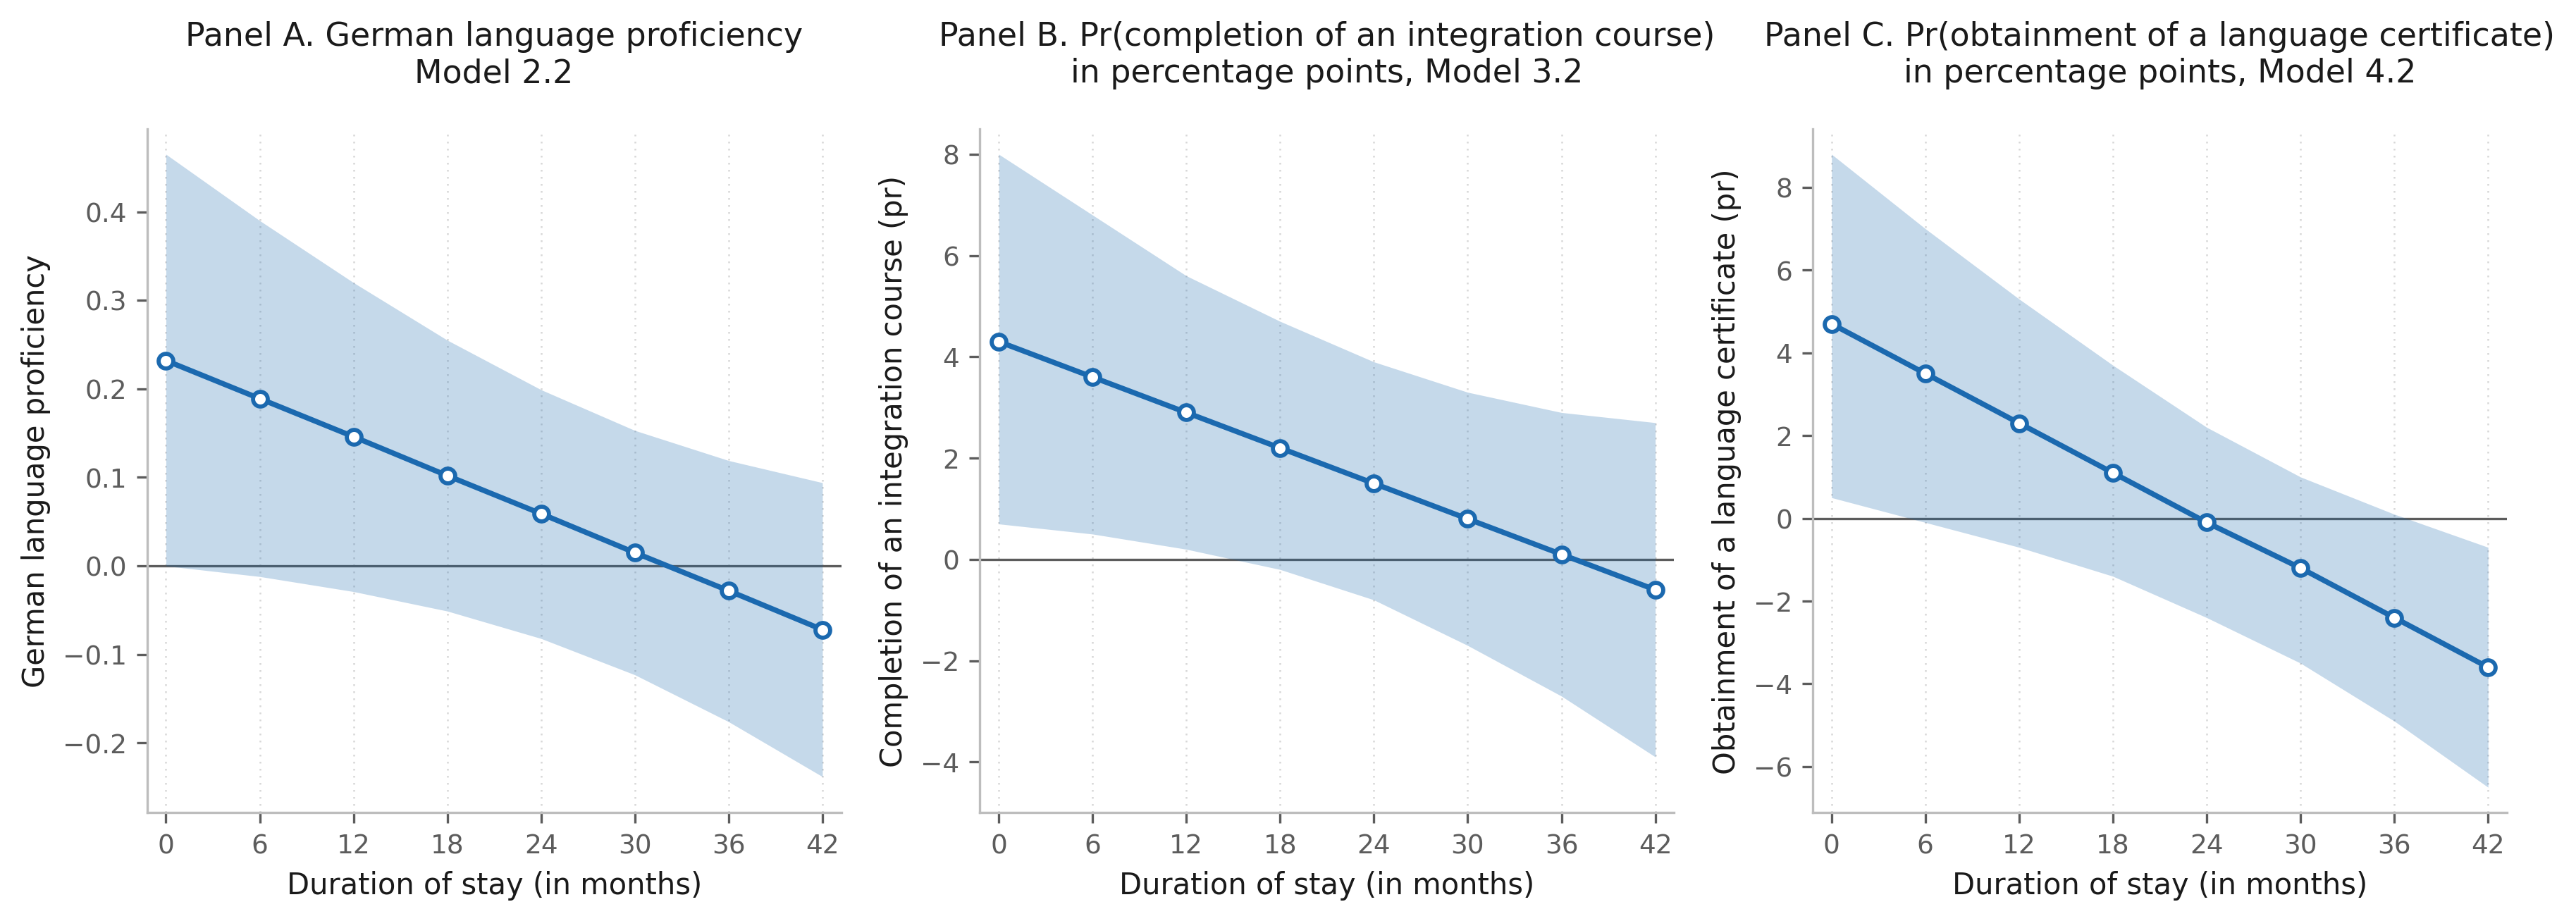
\includegraphics[width=\textwidth]{figures/fig02_all_panels.png}
  \caption[Marginaler Effekt des Kursangebots nach Aufenthaltsdauer]{%
    Durchschnittlicher marginaler Effekt (AME) des Kreisangebots an
    Integrationskursen auf die intermedi\"aren Ergebnisse, nach Aufenthaltsdauer,
    mit 95-\%-Konfidenzintervall. Panel~A: Deutschkenntnisse in Skalenpunkten
    (Modell~2.2); Panel~B: Abschluss eines Integrationskurses in Prozentpunkten
    (Modell~3.2); Panel~C: Erwerb eines Sprachzertifikats in Prozentpunkten
    (Modell~4.2). Zugrunde liegen die Interaktionsmodelle aus
    Tabelle~\ref{tab:intermediaere-ergebnisse}. Eigene Berechnung,
    IAB-BAMF-SOEP-Befragung von Gefl\"uchteten 2016--2019, SOEP-Core v36
    (Remote Edition), gewichtet; N\,=\,5.467 Beobachtungen von 2.730 Personen,
    20~Imputationen. Entspricht Abbildung~2 in \textcite{Kanas:2023}.}
  \label{fig:ame-aufenthaltsdauer}
\end{figure}


\section{Erwerbst\"atigkeit unter Kontrolle der intermedi\"aren Ergebnisse}
\label{sec:erg-mediation}

\textcite{Kanas:2023} haben den Zusammenhang zwischen dem Angebot an Sprachkursen vor Ort und den Beschäftigungschancen von Geflüchteten untersucht und geprüft, ob dieser Zusammenhang auch dann noch besteht, wenn Faktoren wie Kursabschluss, Zertifikat, Deutschkenntnisse und die Häufigkeit des Kontakts zu Deutschen berücksichtigt werden. In Tabelle 5.4 wurde diese Analyse reproduziert, sodass dieselben Ergebnisse ermittelt werden konnten.

Zunächst wird im Modell 1.3 die Deutschkenntnis berücksichtigt. Das Angebot an Kursen erhöht die Beschäftigungswahrscheinlichkeit um fast 3 Prozentpunkte, wenn die Deutschkenntnis dabei berücksichtigt wird. Die Variable „Abschluss des Integrationskurses“ steht in einem positiven Zusammenhang mit der Beschäftigung. Wenn die Variable „Kursabschluss“ in das Modell aufgenommen wird, ist der Effekt des Kursangebots auf die Beschäftigung ebenfalls positiv und statistisch signifikant. Der Besitz eines Deutsch-Sprachzertifikats ist ebenfalls mit einer höheren Beschäftigungswahrscheinlichkeit verbunden, allerdings liegt das statistische Signifikanzniveau bei 10 Prozent. Das bedeutet, dass die Wirkungsstärke dieser Variablen geringer ist als die der Variablen „Abschluss des Integrationskurses“. Auch die Variable „Häufigkeit des Kontakts mit Deutschen“ steht in Zusammenhang mit der Beschäftigungswahrscheinlichkeit, und dieser Zusammenhang ist positiv und signifikant.

In Modell 1.7 und Modell 1.8 wurden mehrere intermediäre Ergebnisse gleichzeitig berücksichtigt. In beiden Modellen lässt sich ein signifikanter und positiver Zusammenhang zwischen der Häufigkeit des Kontakts zu Deutschen und der Beschäftigungswahrscheinlichkeit beobachten. Auch unter Berücksichtigung weiterer intermediärer Variablen blieb der Zusammenhang zwischen der Variable „Kontakt zu Deutschen“ und der Beschäftigungswahrscheinlichkeit stabil. In Modell 1.7 wurde gezeigt, dass der Zusammenhang zwischen dem Abschluss eines Integrationskurses und der Beschäftigungswahrscheinlichkeit auch unter Berücksichtigung der Deutschkenntnisse und der Häufigkeit des Kontakts zu Deutschen signifikant und positiv ist.


% GENERATED BY src/python/lmi/tables/tab05_mediation.py -- DO NOT EDIT
%==============================================================================%
% tab05_mediation.tex
%
% Purpose : Tabelle 5 der Replikation -- Erwerbstaetigkeit unter Kontrolle der
%           intermediaeren Ergebnisse. Entspricht Table 5 in
%           Kanas & Kosyakova, S. 25 (Bib-Key: Kanas:2023).
%           Zweite Tabelle: Gegenueberstellung Publikation vs. Replikation
%           fuer den Anhang.
% Source  : SOEPremote job 244598, src/stata/remote/tab05_mediation.do
%           Rohlisting: results/transcripts/
%                       src_stata_remote_tab05_mediation.do.eml
%           Transkript: results/comparisons/tab05_mediation.md
% Needs   : booktabs, tabularx (beide bereits in bachelorarbeit.sty geladen)
% Usage   : % GENERATED BY src/python/lmi/tables/tab05_mediation.py -- DO NOT EDIT
%==============================================================================%
% tab05_mediation.tex
%
% Purpose : Tabelle 5 der Replikation -- Erwerbstaetigkeit unter Kontrolle der
%           intermediaeren Ergebnisse. Entspricht Table 5 in
%           Kanas & Kosyakova, S. 25 (Bib-Key: Kanas:2023).
%           Zweite Tabelle: Gegenueberstellung Publikation vs. Replikation
%           fuer den Anhang.
% Source  : SOEPremote job 244598, src/stata/remote/tab05_mediation.do
%           Rohlisting: results/transcripts/
%                       src_stata_remote_tab05_mediation.do.eml
%           Transkript: results/comparisons/tab05_mediation.md
% Needs   : booktabs, tabularx (beide bereits in bachelorarbeit.sty geladen)
% Usage   : \input{tables/tab05_mediation}
% Author  : Emre Suemer, 2026-08-14
%==============================================================================%

\makeatletter
\@ifundefined{NC@rewrite@Z}{%
  \newcolumntype{Z}{>{\raggedright\arraybackslash\hangindent=1.9em\hangafter=1}X}%
}{}
\makeatother

\begin{table}[htbp]
  \centering
  \caption{Erwerbst\"atigkeit und intermedi\"are Ergebnisse}
  \label{tab:mediation}
  \scriptsize
  \setlength{\tabcolsep}{3pt}%
  \begin{tabularx}{\textwidth}{@{}Zrrrrrr@{}}
    \toprule
     & Modell 1.3 & Modell 1.4 & Modell 1.5 & Modell 1.6 & Modell 1.7
     & Modell 1.8 \\
    \midrule
    \textbf{Kreisangebot an Integrationskursen, std.} & 2{,}97$^{*}$ & 2{,}93$^{*}$ & 3{,}04$^{*}$ & 3{,}19$^{**}$ & 3{,}13$^{**}$ & 3{,}18$^{**}$ \\
     & (1{,}18) & (1{,}19) & (1{,}19) & (1{,}12) & (1{,}11) & (1{,}12) \\[0.3ex]
    Aufenthaltsdauer, in Monaten (/12) & 9{,}14$^{**}$ & 10{,}29$^{**}$ & 10{,}32$^{**}$ & 9{,}38$^{**}$ & 8{,}53$^{**}$ & 8{,}68$^{**}$ \\
     & (1{,}62) & (1{,}62) & (1{,}65) & (1{,}61) & (1{,}66) & (1{,}67) \\[0.3ex]
    Deutschkenntnisse & 1{,}64$^{**}$ &  &  &  & 0{,}51 & 0{,}68$^{+}$ \\
     & (0{,}36) &  &  &  & (0{,}37) & (0{,}38) \\[0.3ex]
    Integrationskurs abgeschlossen &  & 7{,}62$^{**}$ &  &  & 6{,}73$^{**}$ &  \\
     &  & (2{,}43) &  &  & (2{,}40) &  \\[0.3ex]
    Sprachzertifikat erworben &  &  & 4{,}02$^{+}$ &  &  & 0{,}81 \\
     &  &  & (2{,}20) &  &  & (2{,}15) \\[0.3ex]
    Kontakth\"aufigkeit zu Deutschen &  &  &  & 5{,}06$^{**}$ & 4{,}88$^{**}$ & 4{,}83$^{**}$ \\
     &  &  &  & (0{,}44) & (0{,}45) & (0{,}45) \\[0.3ex]
    Konstante & $-$10{,}45$^{+}$ & $-$3{,}09 & $-$2{,}70 & $-$18{,}86$^{**}$ & $-$21{,}08$^{**}$ & $-$21{,}39$^{**}$ \\
     & (6{,}26) & (6{,}21) & (6{,}28) & (6{,}16) & (6{,}09) & (6{,}14) \\[0.3ex]
    R\textsuperscript{2} (adj.) & 0{,}2209 & 0{,}2186 & 0{,}2147 & 0{,}2563 & 0{,}2614 & 0{,}2575 \\
    \bottomrule
  \end{tabularx}

  \vspace{0.75ex}
  \parbox{\textwidth}{\footnotesize
    \textit{Anmerkungen:} Eigene Berechnung, IAB-BAMF-SOEP-Befragung von
    Gefl\"uchteten 2016--2019, SOEP-Core v36 (Remote Edition), gewichtet.
    In allen Modellen N\,=\,5.467 Beobachtungen, 2.730 Personen,
    20 Imputationen. Durchschnittliche marginale Effekte in
    Prozentpunkten; robuste, auf Personenebene geclusterte Standardfehler in
    Klammern. Die Kontrollvariablen entsprechen exakt denen aus Modell~1.1 in
    Tabelle~\ref{tab:erwerbstaetigkeit} und sind wie in der Vorlage nicht
    ausgewiesen; die vollst\"andigen Koeffizienten stehen in
    \texttt{build/tables/tab05\_mediation.csv}.
    $^{+}$~p\,$<$\,0{,}1, $^{*}$~p\,$<$\,0{,}05, $^{**}$~p\,$<$\,0{,}01
    (zweiseitig).}
\end{table}


\iffalse
\begin{table}[htbp]
  \centering
  \caption{Tabelle~\ref{tab:mediation} im Vergleich zur Publikation}
  \label{tab:mediation-vergleich}
  \scriptsize
  \setlength{\tabcolsep}{3pt}%
  \begin{tabularx}{\textwidth}{@{}Zrrrrrr@{}}
    \toprule
     & Modell 1.3 & Modell 1.4 & Modell 1.5 & Modell 1.6 & Modell 1.7
     & Modell 1.8 \\
    \midrule
    \multicolumn{7}{@{}l}{\textbf{Publikation}} \\[0.3ex]
    \textbf{Kreisangebot an Integrationskursen, std.} & 2{,}96$^{*}$ & 2{,}91$^{*}$ & 3{,}03$^{*}$ & 3{,}18$^{**}$ & 3{,}12$^{**}$ & 3{,}18$^{**}$ \\
     & (1{,}18) & (1{,}19) & (1{,}20) & (1{,}12) & (1{,}11) & (1{,}12) \\[0.3ex]
    Aufenthaltsdauer, in Monaten (/12) & 9{,}13$^{**}$ & 10{,}27$^{**}$ & 10{,}31$^{**}$ & 9{,}37$^{**}$ & 8{,}51$^{**}$ & 8{,}67$^{**}$ \\
     & (1{,}62) & (1{,}62) & (1{,}64) & (1{,}61) & (1{,}66) & (1{,}67) \\[0.3ex]
    Deutschkenntnisse & 1{,}65$^{**}$ &  &  &  & 0{,}51 & 0{,}69$^{+}$ \\
     & (0{,}37) &  &  &  & (0{,}37) & (0{,}38) \\[0.3ex]
    Integrationskurs abgeschlossen &  & 7{,}95$^{**}$ &  &  & 7{,}02$^{**}$ &  \\
     &  & (2{,}41) &  &  & (2{,}38) &  \\[0.3ex]
    Sprachzertifikat erworben &  &  & 4{,}09$^{+}$ &  &  & 0{,}86 \\
     &  &  & (2{,}20) &  &  & (2{,}15) \\[0.3ex]
    Kontakth\"aufigkeit zu Deutschen &  &  &  & 5{,}07$^{**}$ & 4{,}87$^{**}$ & 4{,}83$^{**}$ \\
     &  &  &  & (0{,}44) & (0{,}45) & (0{,}46) \\[0.3ex]
    Konstante & $-$10{,}35$^{+}$ & $-$2{,}87 & $-$2{,}49 & $-$18{,}58$^{**}$ & $-$20{,}83$^{**}$ & $-$21{,}17$^{**}$ \\
     & (6{,}25) & (6{,}19) & (6{,}26) & (6{,}18) & (6{,}12) & (6{,}17) \\[0.3ex]
    R\textsuperscript{2} (adj.) & 0{,}2205 & 0{,}2185 & 0{,}2143 & 0{,}2558 & 0{,}2613 & 0{,}2571 \\
    \midrule
    \multicolumn{7}{@{}l}{\textbf{Replikation}} \\[0.3ex]
    \textbf{Kreisangebot an Integrationskursen, std.} & 2{,}97$^{*}$ & 2{,}93$^{*}$ & 3{,}04$^{*}$ & 3{,}19$^{**}$ & 3{,}13$^{**}$ & 3{,}18$^{**}$ \\
     & (1{,}18) & (1{,}19) & (1{,}19) & (1{,}12) & (1{,}11) & (1{,}12) \\[0.3ex]
    Aufenthaltsdauer, in Monaten (/12) & 9{,}14$^{**}$ & 10{,}29$^{**}$ & 10{,}32$^{**}$ & 9{,}38$^{**}$ & 8{,}53$^{**}$ & 8{,}68$^{**}$ \\
     & (1{,}62) & (1{,}62) & (1{,}65) & (1{,}61) & (1{,}66) & (1{,}67) \\[0.3ex]
    Deutschkenntnisse & 1{,}64$^{**}$ &  &  &  & 0{,}51 & 0{,}68$^{+}$ \\
     & (0{,}36) &  &  &  & (0{,}37) & (0{,}38) \\[0.3ex]
    Integrationskurs abgeschlossen &  & 7{,}62$^{**}$ &  &  & 6{,}73$^{**}$ &  \\
     &  & (2{,}43) &  &  & (2{,}40) &  \\[0.3ex]
    Sprachzertifikat erworben &  &  & 4{,}02$^{+}$ &  &  & 0{,}81 \\
     &  &  & (2{,}20) &  &  & (2{,}15) \\[0.3ex]
    Kontakth\"aufigkeit zu Deutschen &  &  &  & 5{,}06$^{**}$ & 4{,}88$^{**}$ & 4{,}83$^{**}$ \\
     &  &  &  & (0{,}44) & (0{,}45) & (0{,}45) \\[0.3ex]
    Konstante & $-$10{,}45$^{+}$ & $-$3{,}09 & $-$2{,}70 & $-$18{,}86$^{**}$ & $-$21{,}08$^{**}$ & $-$21{,}39$^{**}$ \\
     & (6{,}26) & (6{,}21) & (6{,}28) & (6{,}16) & (6{,}09) & (6{,}14) \\[0.3ex]
    R\textsuperscript{2} (adj.) & 0{,}2209 & 0{,}2186 & 0{,}2147 & 0{,}2563 & 0{,}2614 & 0{,}2575 \\
    \bottomrule
  \end{tabularx}

  \vspace{0.75ex}
  \parbox{\textwidth}{\footnotesize
    \textit{Anmerkungen:} Publizierte Werte aus \textcite[25]{Kanas:2023},
    eigene Werte aus SOEPremote-Job~244598. Einheiten wie oben.
    Gr\"o\ss{}te Abweichung des Treatment-Koeffizienten: 0{,}02\,p.p.;
    gr\"o\ss{}te Abweichung eines Steigungskoeffizienten: 0{,}33\,p.p.;
    gr\"o\ss{}te Abweichung insgesamt: 0{,}33\,p.p.
    Alle Signifikanzniveaus stimmen \"uberein.
    \\[0.4ex]
    \textbf{Anmerkung:} Die Fiskalrechnung der Autorinnen st\"utzt sich auf
    Modell~1.7, nicht auf den Haupteffekt aus
    Tabelle~\ref{tab:erwerbstaetigkeit}: 3{,}13\,p.p. $\times$ 10.000 $\times$ 4.800\,Euro = 1.502.400\,Euro (publiziert: 1.497.600\,Euro).}
\end{table}
\fi
% Author  : Emre Suemer, 2026-08-14
%==============================================================================%

\makeatletter
\@ifundefined{NC@rewrite@Z}{%
  \newcolumntype{Z}{>{\raggedright\arraybackslash\hangindent=1.9em\hangafter=1}X}%
}{}
\makeatother

\begin{table}[htbp]
  \centering
  \caption{Erwerbst\"atigkeit und intermedi\"are Ergebnisse}
  \label{tab:mediation}
  \scriptsize
  \setlength{\tabcolsep}{3pt}%
  \begin{tabularx}{\textwidth}{@{}Zrrrrrr@{}}
    \toprule
     & Modell 1.3 & Modell 1.4 & Modell 1.5 & Modell 1.6 & Modell 1.7
     & Modell 1.8 \\
    \midrule
    \textbf{Kreisangebot an Integrationskursen, std.} & 2{,}97$^{*}$ & 2{,}93$^{*}$ & 3{,}04$^{*}$ & 3{,}19$^{**}$ & 3{,}13$^{**}$ & 3{,}18$^{**}$ \\
     & (1{,}18) & (1{,}19) & (1{,}19) & (1{,}12) & (1{,}11) & (1{,}12) \\[0.3ex]
    Aufenthaltsdauer, in Monaten (/12) & 9{,}14$^{**}$ & 10{,}29$^{**}$ & 10{,}32$^{**}$ & 9{,}38$^{**}$ & 8{,}53$^{**}$ & 8{,}68$^{**}$ \\
     & (1{,}62) & (1{,}62) & (1{,}65) & (1{,}61) & (1{,}66) & (1{,}67) \\[0.3ex]
    Deutschkenntnisse & 1{,}64$^{**}$ &  &  &  & 0{,}51 & 0{,}68$^{+}$ \\
     & (0{,}36) &  &  &  & (0{,}37) & (0{,}38) \\[0.3ex]
    Integrationskurs abgeschlossen &  & 7{,}62$^{**}$ &  &  & 6{,}73$^{**}$ &  \\
     &  & (2{,}43) &  &  & (2{,}40) &  \\[0.3ex]
    Sprachzertifikat erworben &  &  & 4{,}02$^{+}$ &  &  & 0{,}81 \\
     &  &  & (2{,}20) &  &  & (2{,}15) \\[0.3ex]
    Kontakth\"aufigkeit zu Deutschen &  &  &  & 5{,}06$^{**}$ & 4{,}88$^{**}$ & 4{,}83$^{**}$ \\
     &  &  &  & (0{,}44) & (0{,}45) & (0{,}45) \\[0.3ex]
    Konstante & $-$10{,}45$^{+}$ & $-$3{,}09 & $-$2{,}70 & $-$18{,}86$^{**}$ & $-$21{,}08$^{**}$ & $-$21{,}39$^{**}$ \\
     & (6{,}26) & (6{,}21) & (6{,}28) & (6{,}16) & (6{,}09) & (6{,}14) \\[0.3ex]
    R\textsuperscript{2} (adj.) & 0{,}2209 & 0{,}2186 & 0{,}2147 & 0{,}2563 & 0{,}2614 & 0{,}2575 \\
    \bottomrule
  \end{tabularx}

  \vspace{0.75ex}
  \parbox{\textwidth}{\footnotesize
    \textit{Anmerkungen:} Eigene Berechnung, IAB-BAMF-SOEP-Befragung von
    Gefl\"uchteten 2016--2019, SOEP-Core v36 (Remote Edition), gewichtet.
    In allen Modellen N\,=\,5.467 Beobachtungen, 2.730 Personen,
    20 Imputationen. Durchschnittliche marginale Effekte in
    Prozentpunkten; robuste, auf Personenebene geclusterte Standardfehler in
    Klammern. Die Kontrollvariablen entsprechen exakt denen aus Modell~1.1 in
    Tabelle~\ref{tab:erwerbstaetigkeit} und sind wie in der Vorlage nicht
    ausgewiesen; die vollst\"andigen Koeffizienten stehen in
    \texttt{build/tables/tab05\_mediation.csv}.
    $^{+}$~p\,$<$\,0{,}1, $^{*}$~p\,$<$\,0{,}05, $^{**}$~p\,$<$\,0{,}01
    (zweiseitig).}
\end{table}


\iffalse
\begin{table}[htbp]
  \centering
  \caption{Tabelle~\ref{tab:mediation} im Vergleich zur Publikation}
  \label{tab:mediation-vergleich}
  \scriptsize
  \setlength{\tabcolsep}{3pt}%
  \begin{tabularx}{\textwidth}{@{}Zrrrrrr@{}}
    \toprule
     & Modell 1.3 & Modell 1.4 & Modell 1.5 & Modell 1.6 & Modell 1.7
     & Modell 1.8 \\
    \midrule
    \multicolumn{7}{@{}l}{\textbf{Publikation}} \\[0.3ex]
    \textbf{Kreisangebot an Integrationskursen, std.} & 2{,}96$^{*}$ & 2{,}91$^{*}$ & 3{,}03$^{*}$ & 3{,}18$^{**}$ & 3{,}12$^{**}$ & 3{,}18$^{**}$ \\
     & (1{,}18) & (1{,}19) & (1{,}20) & (1{,}12) & (1{,}11) & (1{,}12) \\[0.3ex]
    Aufenthaltsdauer, in Monaten (/12) & 9{,}13$^{**}$ & 10{,}27$^{**}$ & 10{,}31$^{**}$ & 9{,}37$^{**}$ & 8{,}51$^{**}$ & 8{,}67$^{**}$ \\
     & (1{,}62) & (1{,}62) & (1{,}64) & (1{,}61) & (1{,}66) & (1{,}67) \\[0.3ex]
    Deutschkenntnisse & 1{,}65$^{**}$ &  &  &  & 0{,}51 & 0{,}69$^{+}$ \\
     & (0{,}37) &  &  &  & (0{,}37) & (0{,}38) \\[0.3ex]
    Integrationskurs abgeschlossen &  & 7{,}95$^{**}$ &  &  & 7{,}02$^{**}$ &  \\
     &  & (2{,}41) &  &  & (2{,}38) &  \\[0.3ex]
    Sprachzertifikat erworben &  &  & 4{,}09$^{+}$ &  &  & 0{,}86 \\
     &  &  & (2{,}20) &  &  & (2{,}15) \\[0.3ex]
    Kontakth\"aufigkeit zu Deutschen &  &  &  & 5{,}07$^{**}$ & 4{,}87$^{**}$ & 4{,}83$^{**}$ \\
     &  &  &  & (0{,}44) & (0{,}45) & (0{,}46) \\[0.3ex]
    Konstante & $-$10{,}35$^{+}$ & $-$2{,}87 & $-$2{,}49 & $-$18{,}58$^{**}$ & $-$20{,}83$^{**}$ & $-$21{,}17$^{**}$ \\
     & (6{,}25) & (6{,}19) & (6{,}26) & (6{,}18) & (6{,}12) & (6{,}17) \\[0.3ex]
    R\textsuperscript{2} (adj.) & 0{,}2205 & 0{,}2185 & 0{,}2143 & 0{,}2558 & 0{,}2613 & 0{,}2571 \\
    \midrule
    \multicolumn{7}{@{}l}{\textbf{Replikation}} \\[0.3ex]
    \textbf{Kreisangebot an Integrationskursen, std.} & 2{,}97$^{*}$ & 2{,}93$^{*}$ & 3{,}04$^{*}$ & 3{,}19$^{**}$ & 3{,}13$^{**}$ & 3{,}18$^{**}$ \\
     & (1{,}18) & (1{,}19) & (1{,}19) & (1{,}12) & (1{,}11) & (1{,}12) \\[0.3ex]
    Aufenthaltsdauer, in Monaten (/12) & 9{,}14$^{**}$ & 10{,}29$^{**}$ & 10{,}32$^{**}$ & 9{,}38$^{**}$ & 8{,}53$^{**}$ & 8{,}68$^{**}$ \\
     & (1{,}62) & (1{,}62) & (1{,}65) & (1{,}61) & (1{,}66) & (1{,}67) \\[0.3ex]
    Deutschkenntnisse & 1{,}64$^{**}$ &  &  &  & 0{,}51 & 0{,}68$^{+}$ \\
     & (0{,}36) &  &  &  & (0{,}37) & (0{,}38) \\[0.3ex]
    Integrationskurs abgeschlossen &  & 7{,}62$^{**}$ &  &  & 6{,}73$^{**}$ &  \\
     &  & (2{,}43) &  &  & (2{,}40) &  \\[0.3ex]
    Sprachzertifikat erworben &  &  & 4{,}02$^{+}$ &  &  & 0{,}81 \\
     &  &  & (2{,}20) &  &  & (2{,}15) \\[0.3ex]
    Kontakth\"aufigkeit zu Deutschen &  &  &  & 5{,}06$^{**}$ & 4{,}88$^{**}$ & 4{,}83$^{**}$ \\
     &  &  &  & (0{,}44) & (0{,}45) & (0{,}45) \\[0.3ex]
    Konstante & $-$10{,}45$^{+}$ & $-$3{,}09 & $-$2{,}70 & $-$18{,}86$^{**}$ & $-$21{,}08$^{**}$ & $-$21{,}39$^{**}$ \\
     & (6{,}26) & (6{,}21) & (6{,}28) & (6{,}16) & (6{,}09) & (6{,}14) \\[0.3ex]
    R\textsuperscript{2} (adj.) & 0{,}2209 & 0{,}2186 & 0{,}2147 & 0{,}2563 & 0{,}2614 & 0{,}2575 \\
    \bottomrule
  \end{tabularx}

  \vspace{0.75ex}
  \parbox{\textwidth}{\footnotesize
    \textit{Anmerkungen:} Publizierte Werte aus \textcite[25]{Kanas:2023},
    eigene Werte aus SOEPremote-Job~244598. Einheiten wie oben.
    Gr\"o\ss{}te Abweichung des Treatment-Koeffizienten: 0{,}02\,p.p.;
    gr\"o\ss{}te Abweichung eines Steigungskoeffizienten: 0{,}33\,p.p.;
    gr\"o\ss{}te Abweichung insgesamt: 0{,}33\,p.p.
    Alle Signifikanzniveaus stimmen \"uberein.
    \\[0.4ex]
    \textbf{Anmerkung:} Die Fiskalrechnung der Autorinnen st\"utzt sich auf
    Modell~1.7, nicht auf den Haupteffekt aus
    Tabelle~\ref{tab:erwerbstaetigkeit}: 3{,}13\,p.p. $\times$ 10.000 $\times$ 4.800\,Euro = 1.502.400\,Euro (publiziert: 1.497.600\,Euro).}
\end{table}
\fi




%\section{Erweiterte Ergebnisse}
%\label{sec:erw-erg}


\subsection{Ergebnisse der Erweiterung}
\label{sec:erg-erweiterung}

Dieser Abschnitt untersucht, ob sich die Auswirkungen des Kursangebots auf die Beschäftigung je nach Asylstatus der Geflüchteten unterscheiden. \textcite{Kanas:2023} analysierten, ob sich die Auswirkungen des Kursangebots auf die Beschäftigung je nach Asylstatus unterscheiden. Die Erweiterung dieser Studie berücksichtigt die Interaktion zwischen dem lokalen Kursangebot und dem Asylstatus im Hinblick auf die Kursmechanismen. Die Interaktion zwischen dem lokalen Kursangebot und dem Asylstatus wird im Hinblick auf die Auswirkungen auf den Kursabschluss, den Erwerb eines Zertifikats und die Deutschkenntnisse untersucht. Damit wird in dieser Arbeit analysiert, ob Flüchtlinge je nach Asylstatus in unterschiedlichem Maße von lokalen Sprachkursen im Hinblick auf diese Integrationsmechanismen profitieren.

Im ersten Teil dieses Kapitels werden die Ergebnisse dargelegt, ob sich die Auswirkungen des lokalen Kursangebots auf die Beschäftigung je nach Asylstatus unterscheiden. Außerdem wird der marginale Effekt des Kursangebots für jeden einzelnen Asylstatus erläutert. Anhand von Tabelle 5.8 wird die Reproduzierbarkeit der Ergebnisse von \textcite{Kanas:2023} überprüft. In Tabelle 5.9 wurde die Analyse auf die Mechanismen der Integration ausgeweitet und es werden die Ergebnisse zu den marginalen Effekten des Kursangebots je nach Asylstatus dargestellt. Tabelle 5.10 zeigt hingegen die grundlegenden Regressionskoeffizienten sowie die Interaktionseffekte der Mechanismenanalysen. Schließlich zeigt Tabelle 5.11 Ergebnisse dazu, ob die Auswirkungen des Kursangebots auf die Beschäftigung und die Deutschkenntnisse sowohl vom Asylstatus als auch von der Aufenthaltsdauer in Deutschland abhängen.

Tabelle 5.6 zeigt den marginalen Effekt auf die Erwerbstätigkeit in Prozentpunkten. Das Modell E1.1 misst den Asylstatus im Erhebungsjahr. Das Modell E1.2 hingegen misst den Status zum Zeitpunkt der ersten Erhebung. Da im zweiten Modell die zeitliche Abfolge zwischen der Zuweisung zu einem Landkreis und der Asylentscheidung berücksichtigt wird, ist es im Kontext der Forschungsfrage von Bedeutung. Der grundlegende Effekt des Kursangebots erweist sich als positiv und statistisch signifikant. Ein Anstieg des Kursangebots um eine Standardabweichung in dem Kreis, dem eine Person zugeordnet ist, erhöht die Wahrscheinlichkeit einer Beschäftigung um 4,25 Prozentpunkte. Damit wurde das zentrale Ergebnis von Kanas und Kosyakova auch unter erweiterten Bedingungen geprüft.

Im Zusammenhang mit der Forschungsfrage dieser Arbeit spielt die Interaktion zwischen Kursangebot und Asylstatus eine zentrale Rolle. Diese Interaktion ist in beiden Modellen statistisch nicht signifikant (E1.1: −1,28; E1.2: −2,87). Es gibt daher keinen Hinweis darauf, dass die Gruppe „Annerkannt“ im Vergleich zur Referenzgruppe stärker vom Kursangebot beeinflusst wird. Die Annahme, dass anerkannte Geflüchtete stärker vom lokalen Kursangebot profitieren, wird aus diesem Grund nicht gestützt. Außerdem sind die gemeinsamen Interaktionen beider Tests nicht signifikant. Im Modell E1.2 liegt lediglich eine schwache Signifikanz vor (p = 0,084). Der Interaktionseffekt im Modell E1.2 ist bei Personen mit abgelehntem Status negativ und statistisch signifikant (−5,13*). Daraus ergibt sich die Erkenntnis, dass bei Personen mit abgelehntem Asylantrag die Auswirkungen des Kursangebots auf die Beschäftigung im Vergleich zur Referenzgruppe geringer sind.

Insgesamt wurde die Analyse von \textcite{Kanas:2023} mit dem Modell E.1.1 wiederholt und überprüft. Im Modell E1.2 wurde der Asylstatus als erster Beobachtungszustand gemessen. Zusammenfassend lässt sich feststellen, dass der grundlegende Effekt des Kursangebots signifikant ist. Berücksichtigt man jedoch den Asylstatus als erste Beobachtungssituation, ist dieser Effekt statistisch nicht signifikant. Daher lässt sich keine Abhängigkeit des Einflusses des Kursangebots auf die Beschäftigung vom jeweiligen Asylstatus feststellen.

% GENERATED BY src/python/lmi/tables/ext_asyl_employment.py
% -- DO NOT EDIT
%==============================================================================%
% ext_asyl_employment.tex
%
% Purpose : Erweiterung, Tabelle E1 -- Kursangebot x Asylstatus auf die
%           Erwerbstaetigkeit. Drei Tabellen: Koeffizienten, marginale Effekte
%           je Statusgruppe, sowie der Vergleich mit Tabelle S6 Modell 1.1.9
%           der Publikation, die dieser Job mitrepliziert.
% Source  : SOEPremote job 244835, src/stata/remote/ext_asyl_employment.do
%           Rohlisting: results/transcripts/
%                       src_stata_remote_ext_asyl_employment.do.eml
%           Transkript: results/comparisons/ext_asyl_employment.md
% Needs   : booktabs, tabularx (beide bereits in bachelorarbeit.sty geladen)
% Usage   : % GENERATED BY src/python/lmi/tables/ext_asyl_employment.py
% -- DO NOT EDIT
%==============================================================================%
% ext_asyl_employment.tex
%
% Purpose : Erweiterung, Tabelle E1 -- Kursangebot x Asylstatus auf die
%           Erwerbstaetigkeit. Drei Tabellen: Koeffizienten, marginale Effekte
%           je Statusgruppe, sowie der Vergleich mit Tabelle S6 Modell 1.1.9
%           der Publikation, die dieser Job mitrepliziert.
% Source  : SOEPremote job 244835, src/stata/remote/ext_asyl_employment.do
%           Rohlisting: results/transcripts/
%                       src_stata_remote_ext_asyl_employment.do.eml
%           Transkript: results/comparisons/ext_asyl_employment.md
% Needs   : booktabs, tabularx (beide bereits in bachelorarbeit.sty geladen)
% Usage   : \input{tables/ext_asyl_employment}
% Author  : Emre Suemer, 2026-09-01
%==============================================================================%

\makeatletter
\@ifundefined{NC@rewrite@Z}{%
  \newcolumntype{Z}{>{\raggedright\arraybackslash\hangindent=1.9em\hangafter=1}X}%
}{}
\makeatother

\begin{table}[htbp]
  \centering
  \caption{Kursangebot und Asylstatus: Wahrscheinlichkeit bezahlter Arbeit}
  \label{tab:ext-asyl-erwerb}
  \footnotesize
  \setlength{\tabcolsep}{4pt}%
  \begin{tabularx}{\textwidth}{@{}Zrr@{}}
    \toprule
     & Modell E1.1 & Modell E1.2 \\
     & Status im & Status bei \\
     & Erhebungsjahr & Erstbeobachtung \\
     & p.p. (SE) & p.p. (SE) \\
    \midrule
    \textbf{Kreisangebot an Integrationskursen, std.} & 3{,}97$^{*}$ (1{,}55) & 4{,}25$^{**}$ (1{,}31) \\
    \quad $\times$ Anerkannt & $-$1{,}28 (1{,}90) & $-$2{,}87 (2{,}03) \\
    \quad $\times$ Abgelehnt & $-$2{,}56 (2{,}47) & $-$5{,}13$^{*}$ (2{,}55) \\
    Aufenthaltsdauer, in Monaten (/12) & 10{,}73$^{**}$ (1{,}60) & 11{,}37$^{**}$ (1{,}60) \\
    Bildungsjahre vor der Migration & 0{,}56$^{**}$ (0{,}19) & 0{,}57$^{**}$ (0{,}20) \\
    Erwerbserfahrung vor der Migration & 4{,}64$^{+}$ (2{,}38) & 4{,}56$^{+}$ (2{,}39) \\
    Weiblich & $-$15{,}76$^{**}$ (2{,}16) & $-$15{,}69$^{**}$ (2{,}18) \\
    Kinder unter 16 Jahren im Haushalt & $-$11{,}02$^{**}$ (2{,}15) & $-$11{,}27$^{**}$ (2{,}18) \\
    Einreise mit der Familie & 5{,}33$^{**}$ (1{,}97) & 5{,}38$^{**}$ (2{,}01) \\
    Unterst\"utzung durch Familie/Verwandte in DE & 4{,}01 (2{,}83) & 4{,}10 (2{,}90) \\
    Alter bei der Erstbefragung & $-$0{,}35$^{**}$ (0{,}09) & $-$0{,}34$^{**}$ (0{,}09) \\
    Traumatische Erfahrungen & $-$0{,}24 (2{,}31) & $-$0{,}11 (2{,}33) \\
    Status des Asylantrags (Ref.: keine Entscheidung) & & \\
    \quad -- Anerkannt & 5{,}27$^{*}$ (2{,}61) & 5{,}21$^{*}$ (2{,}63) \\
    \quad -- Abgelehnt & 8{,}20$^{**}$ (2{,}76) & 4{,}39 (2{,}95) \\
    Kreisanteil Ausl\"ander:innen, std. & $-$1{,}12 (2{,}79) & $-$0{,}80 (2{,}83) \\
    Kreisbev\"olkerungsdichte, std. & $-$0{,}95 (3{,}61) & $-$1{,}05 (3{,}62) \\
    Kreisarbeitslosenquote, std. & $-$4{,}43$^{+}$ (2{,}43) & $-$3{,}99 (2{,}48) \\
    Kreissorgen \"uber Zuwanderung, std. & 0{,}33 (1{,}19) & 0{,}30 (1{,}21) \\
    Kreisanteil CDU/CSU-W\"ahler:innen, std. & $-$2{,}01 (2{,}20) & $-$1{,}65 (2{,}21) \\
    Konstante & $-$2{,}82 (6{,}31) & $-$4{,}16 (6{,}36) \\
    \midrule
    \multicolumn{3}{@{}l}{\textit{Fixe Effekte}} \\
    \quad Erhebungsjahr, Erhebungsstichprobe & Ja & Ja \\
    \quad Bundesland, Herkunftsland (aggregiert) & Ja & Ja \\
    \midrule
    Gemeinsamer Test beider Interaktionen & F(2; 2726{,}6)\,=\,0{,}57 & F(2; 2726{,}9)\,=\,2{,}48 \\
    \quad p & 0{,}563 & 0{,}084 \\
    \midrule
    N Beobachtungen & 5.467 & 5.467 \\
    N Personen & 2.730 & 2.730 \\
    N Imputationen & 20 & 20 \\
    R\textsuperscript{2} (adj.) & 0{,}2137 & 0{,}2121 \\
    \bottomrule
  \end{tabularx}

  \vspace{0.75ex}
  \parbox{\textwidth}{\footnotesize
    \textit{Anmerkungen:} Eigene Berechnung, IAB-BAMF-SOEP-Befragung von
    Gefl\"uchteten 2016--2019, SOEP-Core v36 (Remote Edition), gewichtet.  $^{+}$~p\,$<$\,0{,}1, $^{*}$~p\,$<$\,0{,}05, $^{**}$~p\,$<$\,0{,}01
    (zweiseitig).}
    
	%   Spezifikation wie Modell~1.1 in Tabelle~\ref{tab:erwerbstaetigkeit},
	%   erg\"anzt um die Interaktion des Kursangebots mit dem Asylstatus.
	%   Lineare Wahrscheinlichkeitsmodelle, durchschnittliche marginale Effekte in
	%   Prozentpunkten; robuste, auf Personenebene geclusterte Standardfehler in
	%   Klammern. Referenzkategorie des Asylstatus ist \glqq keine
	%   Entscheidung\grqq{}; die Kategorien sind gegen\"uber der Publikation
	%   korrigiert (vgl.\ Tabelle~\ref{tab:erwerbstaetigkeit}).
	%   Modell~E1.1 misst den Status im jeweiligen Erhebungsjahr, Modell~E1.2 bei
	%   der Erstbeobachtung der Person -- Letzteres ist konzeptionell sauberer,
	%   weil Asylentscheidungen erst \emph{nach} der Kreiszuweisung ergehen
	%   (Tabelle~\ref{tab:ext-asyl-uebergang}). In Spalte~E1.2 beziehen sich
	%   sowohl die Interaktions- als auch die Haupteffektzeilen des Asylstatus
	%   entsprechend auf den Status bei Erstbeobachtung.
    
\end{table}

\begin{table}[htbp]
  \centering
  \caption{Marginaler Effekt des Kursangebots auf die Erwerbst\"atigkeit,
           nach Asylstatus}
  \label{tab:ext-asyl-erwerb-ame}
  \footnotesize
  \setlength{\tabcolsep}{4pt}%
  \begin{tabularx}{\textwidth}{@{}Zrrrr@{}}
    \toprule
     & \multicolumn{2}{c}{Modell E1.1: Erhebungsjahr}
     & \multicolumn{2}{c}{Modell E1.2: Erstbeobachtung} \\
    \cmidrule(lr){2-3}\cmidrule(lr){4-5}
    Status des Asylantrags & p.p. (SE) & p & p.p. (SE) & p \\
    \midrule
    Keine Entscheidung & 4{,}0$^{*}$ (1{,}5) & 0{,}010 & 4{,}3$^{**}$ (1{,}3) & 0{,}001 \\
    Anerkannt & 2{,}7$^{+}$ (1{,}5) & 0{,}078 & 1{,}4 (1{,}9) & 0{,}467 \\
    Abgelehnt & 1{,}4 (2{,}2) & 0{,}519 & $-$0{,}9 (2{,}4) & 0{,}720 \\
    \midrule
    Gemeinsamer Test & \multicolumn{2}{c}{F(2; 2726{,}6)\,=\,0{,}57, p\,=\,0{,}563}
     & \multicolumn{2}{c}{F(2; 2726{,}9)\,=\,2{,}48, p\,=\,0{,}084} \\
    \bottomrule
  \end{tabularx}

  \vspace{0.75ex}
  \parbox{\textwidth}{\footnotesize
    \textit{Anmerkungen:} Durchschnittliche marginale Effekte einer Erh\"ohung
    des Kreisangebots um eine Standardabweichung auf die Wahrscheinlichkeit
    bezahlter Arbeit, in Prozentpunkten, aus den Modellen der
    Tabelle~\ref{tab:ext-asyl-erwerb} (\texttt{mimrgns}, Poolung nach Rubins
    Regeln). Kontrolliert ist die Identit\"at
    AME(Gruppe)\,=\,$b$[Angebot]\,$+$\,$b$[Angebot\,$\times$\,Gruppe];
    gr\"o\ss{}te Abweichung zwischen beiden Rechenwegen 0{,}050~p.p.
    \\[0.4ex]
    \textbf{Inferenzregel, vorab festgelegt} (Designdokument, Abschnitt~3e):
    Prim\"ar ist der gemeinsame Test beider Interaktionsterme, einzelne
    Kontraste sind deskriptiv. \emph{Keine} der beiden Spezifikationen
    erreicht p\,$<$\,0{,}05. Der einzelne signifikante Kontrast in
    Modell~E1.2 darf daher nicht als Befund berichtet werden.
    \\[0.4ex]
    \textbf{Statistische Power, ebenfalls vorab festgehalten:} Bei
    Gruppenanteilen von 39/38/23~Prozent liegen die Standardfehler der
    Subgruppen etwa beim 1{,}6- bis 2{,}1-Fachen des gepoolten Werts von
    1{,}19. Ein Unterschied unter rund 4~Prozentpunkten ist auf dieser
    Ergebnisstufe nicht nachweisbar. Die Aussage lautet deshalb nicht
    \glqq es gibt keinen Effekt\grqq{}, sondern: ein Effekt dieser
    Gr\"o\ss{}enordnung h\"atte hier nicht entdeckt werden k\"onnen.
    Die Erweiterung wird auf der Mechanismenstufe entschieden
    (Tabelle~\ref{tab:ext-asyl-mechanismen}).}
\end{table}

\begin{table}[htbp]
  \centering
  \caption{Modell~E1.1 im Vergleich zu Tabelle~S6, Modell~1.1.9 der
           Publikation}
  \label{tab:ext-asyl-s6}
  \footnotesize
  \setlength{\tabcolsep}{4pt}%
  \begin{tabularx}{\textwidth}{@{}Zrrr@{}}
    \toprule
     & Publikation & Replikation & Abweichung \\
    \midrule
    Kreisangebot, std. (d.\,h.\ f\"ur \glqq keine Entscheidung\grqq{}) & 3{,}98$^{*}$ (1{,}55) & 3{,}97$^{*}$ (1{,}55) & 0{,}01 \\
    \quad $\times$ Anerkannt & $-$1{,}30 (1{,}90) & $-$1{,}28 (1{,}90) & 0{,}02 \\
    \quad $\times$ Abgelehnt & $-$2{,}58 (2{,}48) & $-$2{,}56 (2{,}47) & 0{,}02 \\
    \midrule
    N Beobachtungen & 5.473 & 5.467 & 6 \\
    N Personen & 2.732 & 2.730 & 2 \\
    \bottomrule
  \end{tabularx}

  \vspace{0.75ex}
  \parbox{\textwidth}{\footnotesize
    \textit{Anmerkungen:} Publizierte Werte aus dem Zusatzmaterial zu
    \textcite{Kanas:2023}, S.~12, Tabelle~S6, Modell~1.1.9; eigene Werte aus
    SOEPremote-Job~244835 (Modell~E1.1). Die Autorinnen sch\"atzen dort exakt
    diese Spezifikation, weshalb Modell~E1.1 zugleich eine Replikation von
    S6 ist. Alle drei Koeffizienten stimmen bis auf 0{,}02~p.p.
    \"uberein, die Standardfehler bis auf 0{,}01, und die Signifikanzniveaus
    vollst\"andig -- dieselbe Toleranz wie in den f\"unf Haupttabellen; die
    Differenz ist Monte-Carlo-Variation der multiplen Imputation.
    \\[0.4ex]
    \textbf{Vierter Fehler in der Publikation:} Tabelle~S6 weist
    5.473 Beobachtungen und 2.732 Personen aus, w\"ahrend die Tabellen~3
    bis~5 auf derselben Stichprobe und mit denselben Kontrollvariablen
    5.467 und 2.730 ausweisen. Die Nachsch\"atzung ergibt 5.467/2.730,
    passend zum Stichprobentrichter
    (Tabelle~\ref{tab:stichprobenselektion}). Die sechs zus\"atzlichen
    Personenjahre und zwei zus\"atzlichen Personen in S6 existieren nicht.
    Die Sch\"atzwerte sind davon unber\"uhrt.}
\end{table}

% Author  : Emre Suemer, 2026-09-01
%==============================================================================%

\makeatletter
\@ifundefined{NC@rewrite@Z}{%
  \newcolumntype{Z}{>{\raggedright\arraybackslash\hangindent=1.9em\hangafter=1}X}%
}{}
\makeatother

\begin{table}[htbp]
  \centering
  \caption{Kursangebot und Asylstatus: Wahrscheinlichkeit bezahlter Arbeit}
  \label{tab:ext-asyl-erwerb}
  \footnotesize
  \setlength{\tabcolsep}{4pt}%
  \begin{tabularx}{\textwidth}{@{}Zrr@{}}
    \toprule
     & Modell E1.1 & Modell E1.2 \\
     & Status im & Status bei \\
     & Erhebungsjahr & Erstbeobachtung \\
     & p.p. (SE) & p.p. (SE) \\
    \midrule
    \textbf{Kreisangebot an Integrationskursen, std.} & 3{,}97$^{*}$ (1{,}55) & 4{,}25$^{**}$ (1{,}31) \\
    \quad $\times$ Anerkannt & $-$1{,}28 (1{,}90) & $-$2{,}87 (2{,}03) \\
    \quad $\times$ Abgelehnt & $-$2{,}56 (2{,}47) & $-$5{,}13$^{*}$ (2{,}55) \\
    Aufenthaltsdauer, in Monaten (/12) & 10{,}73$^{**}$ (1{,}60) & 11{,}37$^{**}$ (1{,}60) \\
    Bildungsjahre vor der Migration & 0{,}56$^{**}$ (0{,}19) & 0{,}57$^{**}$ (0{,}20) \\
    Erwerbserfahrung vor der Migration & 4{,}64$^{+}$ (2{,}38) & 4{,}56$^{+}$ (2{,}39) \\
    Weiblich & $-$15{,}76$^{**}$ (2{,}16) & $-$15{,}69$^{**}$ (2{,}18) \\
    Kinder unter 16 Jahren im Haushalt & $-$11{,}02$^{**}$ (2{,}15) & $-$11{,}27$^{**}$ (2{,}18) \\
    Einreise mit der Familie & 5{,}33$^{**}$ (1{,}97) & 5{,}38$^{**}$ (2{,}01) \\
    Unterst\"utzung durch Familie/Verwandte in DE & 4{,}01 (2{,}83) & 4{,}10 (2{,}90) \\
    Alter bei der Erstbefragung & $-$0{,}35$^{**}$ (0{,}09) & $-$0{,}34$^{**}$ (0{,}09) \\
    Traumatische Erfahrungen & $-$0{,}24 (2{,}31) & $-$0{,}11 (2{,}33) \\
    Status des Asylantrags (Ref.: keine Entscheidung) & & \\
    \quad -- Anerkannt & 5{,}27$^{*}$ (2{,}61) & 5{,}21$^{*}$ (2{,}63) \\
    \quad -- Abgelehnt & 8{,}20$^{**}$ (2{,}76) & 4{,}39 (2{,}95) \\
    Kreisanteil Ausl\"ander:innen, std. & $-$1{,}12 (2{,}79) & $-$0{,}80 (2{,}83) \\
    Kreisbev\"olkerungsdichte, std. & $-$0{,}95 (3{,}61) & $-$1{,}05 (3{,}62) \\
    Kreisarbeitslosenquote, std. & $-$4{,}43$^{+}$ (2{,}43) & $-$3{,}99 (2{,}48) \\
    Kreissorgen \"uber Zuwanderung, std. & 0{,}33 (1{,}19) & 0{,}30 (1{,}21) \\
    Kreisanteil CDU/CSU-W\"ahler:innen, std. & $-$2{,}01 (2{,}20) & $-$1{,}65 (2{,}21) \\
    Konstante & $-$2{,}82 (6{,}31) & $-$4{,}16 (6{,}36) \\
    \midrule
    \multicolumn{3}{@{}l}{\textit{Fixe Effekte}} \\
    \quad Erhebungsjahr, Erhebungsstichprobe & Ja & Ja \\
    \quad Bundesland, Herkunftsland (aggregiert) & Ja & Ja \\
    \midrule
    Gemeinsamer Test beider Interaktionen & F(2; 2726{,}6)\,=\,0{,}57 & F(2; 2726{,}9)\,=\,2{,}48 \\
    \quad p & 0{,}563 & 0{,}084 \\
    \midrule
    N Beobachtungen & 5.467 & 5.467 \\
    N Personen & 2.730 & 2.730 \\
    N Imputationen & 20 & 20 \\
    R\textsuperscript{2} (adj.) & 0{,}2137 & 0{,}2121 \\
    \bottomrule
  \end{tabularx}

  \vspace{0.75ex}
  \parbox{\textwidth}{\footnotesize
    \textit{Anmerkungen:} Eigene Berechnung, IAB-BAMF-SOEP-Befragung von
    Gefl\"uchteten 2016--2019, SOEP-Core v36 (Remote Edition), gewichtet.  $^{+}$~p\,$<$\,0{,}1, $^{*}$~p\,$<$\,0{,}05, $^{**}$~p\,$<$\,0{,}01
    (zweiseitig).}
    
	%   Spezifikation wie Modell~1.1 in Tabelle~\ref{tab:erwerbstaetigkeit},
	%   erg\"anzt um die Interaktion des Kursangebots mit dem Asylstatus.
	%   Lineare Wahrscheinlichkeitsmodelle, durchschnittliche marginale Effekte in
	%   Prozentpunkten; robuste, auf Personenebene geclusterte Standardfehler in
	%   Klammern. Referenzkategorie des Asylstatus ist \glqq keine
	%   Entscheidung\grqq{}; die Kategorien sind gegen\"uber der Publikation
	%   korrigiert (vgl.\ Tabelle~\ref{tab:erwerbstaetigkeit}).
	%   Modell~E1.1 misst den Status im jeweiligen Erhebungsjahr, Modell~E1.2 bei
	%   der Erstbeobachtung der Person -- Letzteres ist konzeptionell sauberer,
	%   weil Asylentscheidungen erst \emph{nach} der Kreiszuweisung ergehen
	%   (Tabelle~\ref{tab:ext-asyl-uebergang}). In Spalte~E1.2 beziehen sich
	%   sowohl die Interaktions- als auch die Haupteffektzeilen des Asylstatus
	%   entsprechend auf den Status bei Erstbeobachtung.
    
\end{table}

\begin{table}[htbp]
  \centering
  \caption{Marginaler Effekt des Kursangebots auf die Erwerbst\"atigkeit,
           nach Asylstatus}
  \label{tab:ext-asyl-erwerb-ame}
  \footnotesize
  \setlength{\tabcolsep}{4pt}%
  \begin{tabularx}{\textwidth}{@{}Zrrrr@{}}
    \toprule
     & \multicolumn{2}{c}{Modell E1.1: Erhebungsjahr}
     & \multicolumn{2}{c}{Modell E1.2: Erstbeobachtung} \\
    \cmidrule(lr){2-3}\cmidrule(lr){4-5}
    Status des Asylantrags & p.p. (SE) & p & p.p. (SE) & p \\
    \midrule
    Keine Entscheidung & 4{,}0$^{*}$ (1{,}5) & 0{,}010 & 4{,}3$^{**}$ (1{,}3) & 0{,}001 \\
    Anerkannt & 2{,}7$^{+}$ (1{,}5) & 0{,}078 & 1{,}4 (1{,}9) & 0{,}467 \\
    Abgelehnt & 1{,}4 (2{,}2) & 0{,}519 & $-$0{,}9 (2{,}4) & 0{,}720 \\
    \midrule
    Gemeinsamer Test & \multicolumn{2}{c}{F(2; 2726{,}6)\,=\,0{,}57, p\,=\,0{,}563}
     & \multicolumn{2}{c}{F(2; 2726{,}9)\,=\,2{,}48, p\,=\,0{,}084} \\
    \bottomrule
  \end{tabularx}

  \vspace{0.75ex}
  \parbox{\textwidth}{\footnotesize
    \textit{Anmerkungen:} Durchschnittliche marginale Effekte einer Erh\"ohung
    des Kreisangebots um eine Standardabweichung auf die Wahrscheinlichkeit
    bezahlter Arbeit, in Prozentpunkten, aus den Modellen der
    Tabelle~\ref{tab:ext-asyl-erwerb} (\texttt{mimrgns}, Poolung nach Rubins
    Regeln). Kontrolliert ist die Identit\"at
    AME(Gruppe)\,=\,$b$[Angebot]\,$+$\,$b$[Angebot\,$\times$\,Gruppe];
    gr\"o\ss{}te Abweichung zwischen beiden Rechenwegen 0{,}050~p.p.
    \\[0.4ex]
    \textbf{Inferenzregel, vorab festgelegt} (Designdokument, Abschnitt~3e):
    Prim\"ar ist der gemeinsame Test beider Interaktionsterme, einzelne
    Kontraste sind deskriptiv. \emph{Keine} der beiden Spezifikationen
    erreicht p\,$<$\,0{,}05. Der einzelne signifikante Kontrast in
    Modell~E1.2 darf daher nicht als Befund berichtet werden.
    \\[0.4ex]
    \textbf{Statistische Power, ebenfalls vorab festgehalten:} Bei
    Gruppenanteilen von 39/38/23~Prozent liegen die Standardfehler der
    Subgruppen etwa beim 1{,}6- bis 2{,}1-Fachen des gepoolten Werts von
    1{,}19. Ein Unterschied unter rund 4~Prozentpunkten ist auf dieser
    Ergebnisstufe nicht nachweisbar. Die Aussage lautet deshalb nicht
    \glqq es gibt keinen Effekt\grqq{}, sondern: ein Effekt dieser
    Gr\"o\ss{}enordnung h\"atte hier nicht entdeckt werden k\"onnen.
    Die Erweiterung wird auf der Mechanismenstufe entschieden
    (Tabelle~\ref{tab:ext-asyl-mechanismen}).}
\end{table}

\begin{table}[htbp]
  \centering
  \caption{Modell~E1.1 im Vergleich zu Tabelle~S6, Modell~1.1.9 der
           Publikation}
  \label{tab:ext-asyl-s6}
  \footnotesize
  \setlength{\tabcolsep}{4pt}%
  \begin{tabularx}{\textwidth}{@{}Zrrr@{}}
    \toprule
     & Publikation & Replikation & Abweichung \\
    \midrule
    Kreisangebot, std. (d.\,h.\ f\"ur \glqq keine Entscheidung\grqq{}) & 3{,}98$^{*}$ (1{,}55) & 3{,}97$^{*}$ (1{,}55) & 0{,}01 \\
    \quad $\times$ Anerkannt & $-$1{,}30 (1{,}90) & $-$1{,}28 (1{,}90) & 0{,}02 \\
    \quad $\times$ Abgelehnt & $-$2{,}58 (2{,}48) & $-$2{,}56 (2{,}47) & 0{,}02 \\
    \midrule
    N Beobachtungen & 5.473 & 5.467 & 6 \\
    N Personen & 2.732 & 2.730 & 2 \\
    \bottomrule
  \end{tabularx}

  \vspace{0.75ex}
  \parbox{\textwidth}{\footnotesize
    \textit{Anmerkungen:} Publizierte Werte aus dem Zusatzmaterial zu
    \textcite{Kanas:2023}, S.~12, Tabelle~S6, Modell~1.1.9; eigene Werte aus
    SOEPremote-Job~244835 (Modell~E1.1). Die Autorinnen sch\"atzen dort exakt
    diese Spezifikation, weshalb Modell~E1.1 zugleich eine Replikation von
    S6 ist. Alle drei Koeffizienten stimmen bis auf 0{,}02~p.p.
    \"uberein, die Standardfehler bis auf 0{,}01, und die Signifikanzniveaus
    vollst\"andig -- dieselbe Toleranz wie in den f\"unf Haupttabellen; die
    Differenz ist Monte-Carlo-Variation der multiplen Imputation.
    \\[0.4ex]
    \textbf{Vierter Fehler in der Publikation:} Tabelle~S6 weist
    5.473 Beobachtungen und 2.732 Personen aus, w\"ahrend die Tabellen~3
    bis~5 auf derselben Stichprobe und mit denselben Kontrollvariablen
    5.467 und 2.730 ausweisen. Die Nachsch\"atzung ergibt 5.467/2.730,
    passend zum Stichprobentrichter
    (Tabelle~\ref{tab:stichprobenselektion}). Die sechs zus\"atzlichen
    Personenjahre und zwei zus\"atzlichen Personen in S6 existieren nicht.
    Die Sch\"atzwerte sind davon unber\"uhrt.}
\end{table}


In Tabelle 5.7 sind die gruppenspezifischen marginalen Effekte des lokalen Kursangebots auf die Beschäftigung dargestellt. Diese Tabelle zeigt sowohl die Ergebnisse zum Asylstatus im Erhebungsjahr (E1.1) als auch zum Asylstatus zum Zeitpunkt der ersten Beobachtung (E1.2). Für die Referenzgruppe „keine Entscheidung“ wurde der Einfluss des Kursangebots mit 4,3 Prozentpunkten ermittelt, wobei das Ergebnis statistisch signifikant ist (P = 0,001). Der geschätzte Einfluss für die Gruppe mit anerkanntem Asylstatus beträgt 1,4 Prozentpunkte, für die Gruppe mit abgelehntem Antrag hingegen -0,9. Beide Effekte sind statistisch nicht signifikant. Zusammenfassend lässt sich feststellen, dass es keine nachgewiesene Heterogenität der Auswirkungen des Kursangebots auf die Beschäftigung in Abhängigkeit vom Asylstatus besteht. Schließlich zeigt Tabelle 5.8 einen Vergleich der reproduzierten Werte mit den Werten aus dem Originalartikel.

% GENERATED BY src/python/lmi/tables/ext_asyl_mediators.py
% -- DO NOT EDIT
%==============================================================================%
% ext_asyl_mediators.tex
%
% Purpose : Erweiterung, Tabelle E2 -- Kursangebot x Asylstatus auf die fuenf
%           Mechanismen. Kern der Erweiterung: getestet wird nicht der Ertrag
%           der Sprache, sondern der Zugang zur Behandlung selbst.
% Source  : SOEPremote jobs 244836, 244837, 244840,
%           src/stata/remote/ext_asyl_mediators_primary.do,
%           ext_asyl_mediators_secondary.do, ext_asyl_participation.do
%           Rohlistings: results/transcripts/src_stata_remote_ext_asyl_*.eml
%           Transkript: results/comparisons/ext_asyl_mediators.md
% Needs   : booktabs, tabularx (beide bereits in bachelorarbeit.sty geladen)
% Usage   : % GENERATED BY src/python/lmi/tables/ext_asyl_mediators.py
% -- DO NOT EDIT
%==============================================================================%
% ext_asyl_mediators.tex
%
% Purpose : Erweiterung, Tabelle E2 -- Kursangebot x Asylstatus auf die fuenf
%           Mechanismen. Kern der Erweiterung: getestet wird nicht der Ertrag
%           der Sprache, sondern der Zugang zur Behandlung selbst.
% Source  : SOEPremote jobs 244836, 244837, 244840,
%           src/stata/remote/ext_asyl_mediators_primary.do,
%           ext_asyl_mediators_secondary.do, ext_asyl_participation.do
%           Rohlistings: results/transcripts/src_stata_remote_ext_asyl_*.eml
%           Transkript: results/comparisons/ext_asyl_mediators.md
% Needs   : booktabs, tabularx (beide bereits in bachelorarbeit.sty geladen)
% Usage   : \input{tables/ext_asyl_mediators}
% Author  : Emre Suemer, 2026-09-01
%==============================================================================%

\makeatletter
\@ifundefined{NC@rewrite@Z}{%
  \newcolumntype{Z}{>{\raggedright\arraybackslash\hangindent=1.9em\hangafter=1}X}%
}{}
\makeatother

\begin{table}[htbp]
  \centering
  \caption{Marginaler Effekt des Kursangebots auf die Mechanismen,
           nach Asylstatus}
  \label{tab:ext-asyl-mechanismen}
  \footnotesize
  \setlength{\tabcolsep}{4pt}%
  \begin{tabularx}{\textwidth}{@{}Zrrrrr@{}}
    \toprule
     & Keine & & & Gemeins. & \\
    Abh\"angige Variable & Entscheidung & Anerkannt & Abgelehnt & Test $p$
     & Form \\
    \midrule
    Integrationskurs besucht & 0{,}008 (0{,}018) & 0{,}038$^{+}$ (0{,}020) & $-$0{,}035 (0{,}026) & 0{,}053 & H1 \\
    Sprachzertifikat erworben & $-$0{,}006 (0{,}016) & $-$0{,}001 (0{,}015) & $-$0{,}047$^{*}$ (0{,}019) & 0{,}105 & H1 \\
    Integrationskurs abgeschlossen & 0{,}013 (0{,}016) & 0{,}024 (0{,}021) & $-$0{,}027 (0{,}026) & 0{,}233 & H1 \\
    Kontakth\"aufigkeit zu Deutschen \textit{(Placebo)} & $-$0{,}001 (0{,}038) & $-$0{,}011 (0{,}036) & $-$0{,}065 (0{,}052) & 0{,}508 & -- \\
    Deutschkenntnisse & 0{,}048 (0{,}096) & $-$0{,}034 (0{,}099) & $-$0{,}022 (0{,}118) & 0{,}763 & -- \\
    \bottomrule
  \end{tabularx}

  \vspace{0.75ex}
  \parbox{\textwidth}{\footnotesize
    \textit{Anmerkungen:} Eigene Berechnung, IAB-BAMF-SOEP-Befragung von
    Gefl\"uchteten 2016--2019, SOEP-Core v36 (Remote Edition), gewichtet.
    
    
%    Je Modell N\,=\,5.467 Beobachtungen, 2.730 Personen, 20 Imputationen.
%    Ausgewiesen ist der durchschnittliche marginale Effekt einer Erh\"ohung
%    des Kreisangebots um eine Standardabweichung auf die jeweilige abh\"angige
%    Variable, gesch\"atzt in der Spezifikation der
%    Tabelle~\ref{tab:intermediaere-ergebnisse} zuz\"uglich der Interaktion mit
%    dem Asylstatus (\texttt{mimrgns}, Poolung nach Rubins Regeln).
    
    
%    Standardfehler in Klammern. \textbf{Rohe Einheiten, keine Prozentpunkte},
%    da die f\"unf abh\"angigen Variablen unterschiedlich skaliert sind: die
%    drei bin\"aren Variablen sind Wahrscheinlichkeiten (0{,}01\,=\,1~p.p.),
%    Deutschkenntnisse Skalenpunkte, Kontakth\"aufigkeit standardisiert.
%    Die Spalte \glqq Form\grqq{} gibt an, welcher Hypothese die Rangfolge der
%    drei Punktsch\"atzer entspricht: H1 (Motivation/Anspruch) sagt
%    abgelehnt\,$<$\,keine Entscheidung\,$<$\,anerkannt voraus, H2
%    (Rationierung) ein Maximum bei \glqq keine Entscheidung\grqq{}.
%    Kontrolliert ist die Identit\"at
%    AME(Gruppe)\,=\,$b$[Angebot]\,$+$\,$b$[Angebot\,$\times$\,Gruppe] gegen
%    \texttt{mimrgns}; gr\"o\ss{}te Abweichung zwischen beiden Rechenwegen
%    0{,}0005.
%    $^{+}$~p\,$<$\,0{,}1, $^{*}$~p\,$<$\,0{,}05, $^{**}$~p\,$<$\,0{,}01
%    (zweiseitig).
    
    
  
%  \\[0.4ex]
%  \textbf{Inferenzregel, vorab festgelegt} (Designdokument, Abschnitt~3e):
%  Prim\"ar ist je Ergebnis der gemeinsame Test beider Interaktionsterme,
%  einzelne Kontraste sind deskriptiv, dazu die Holm-Korrektur \"uber die
%  f\"unf Ergebnisse. \emph{Kein} Ergebnis erreicht p\,$<$\,0{,}05; die
%  Kursteilnahme kommt mit p\,=\,0{,}053 am n\"achsten. Die Holm-Prozedur
%  verwirft nichts: sortierte p-Werte 0{,}053; 0{,}105; 0{,}233; 0{,}508; 0{,}763 gegen die Schwellen
%  0{,}010; 0{,}013; 0{,}017; 0{,}025; 0{,}050 -- bereits der erste Vergleich scheitert, womit das Verfahren
%  endet. Berichtet werden darf, dass die Punktsch\"atzer auf der
%  Teilnahmestufe monoton mit dem rechtlichen Anspruch geordnet sind, nicht
%  aber ein einzelner signifikanter Kontrast.
%  \\[0.4ex]
%  \textbf{Zur Lesart:} Die Kursteilnahme ist der sch\"arfste Test -- ein
%  einziges kausales Glied statt vier, gemessen im Moment der Einschreibung
%  und am wenigsten imputationsabh\"angig (39 unvollst\"andige
%  Beobachtungen gegen\"uber 270 beim Kursabschluss). Das Placebo
%  verh\"alt sich wie ein Placebo: bei der Kontakth\"aufigkeit findet bereits
%  die Vorlage keinen Angebotseffekt, und eine signifikante Moderation dort
%  h\"atte nahegelegt, dass die Interaktion etwas anderes als den
%  differenzierten Kurszugang aufgreift.
    
    
    }
\end{table}

\begin{table}[htbp]
  \centering
  \caption{Kursangebot und Asylstatus: Koeffizienten der Mechanismenmodelle}
  \label{tab:ext-asyl-mechanismen-koef}
  \scriptsize
  \setlength{\tabcolsep}{3pt}%
  \begin{tabularx}{\textwidth}{@{}Zrrrrr@{}}
    \toprule
     & (1) & (2) & (3) & (4) & (5) \\
    Abh\"angige Variable & Teil- & Zerti- & Ab- & Kon- & Deutsch- \\
     & nahme & fikat & schluss & takt & kenntnisse \\
    \midrule
    \textbf{Kreisangebot an Integrationskursen, std.} & 0{,}0084 & $-$0{,}0056 & 0{,}0132 & $-$0{,}0006 & 0{,}0484 \\
     & (0{,}0181) & (0{,}0165) & (0{,}0158) & (0{,}0377) & (0{,}0964) \\[0.3ex]
    \quad $\times$ Anerkannt & 0{,}0299 & 0{,}0042 & 0{,}0112 & $-$0{,}0101 & $-$0{,}0829 \\
     & (0{,}0236) & (0{,}0190) & (0{,}0228) & (0{,}0439) & (0{,}1224) \\[0.3ex]
    \quad $\times$ Abgelehnt & $-$0{,}0431 & $-$0{,}0419$^{+}$ & $-$0{,}0402 & $-$0{,}0644 & $-$0{,}0705 \\
     & (0{,}0301) & (0{,}0234) & (0{,}0281) & (0{,}0559) & (0{,}1369) \\[0.3ex]
    Aufenthaltsdauer, in Monaten (/12) & 0{,}0361$^{+}$ & 0{,}1069$^{**}$ & 0{,}0591$^{**}$ & 0{,}1362$^{**}$ & 0{,}9839$^{**}$ \\
     & (0{,}0214) & (0{,}0161) & (0{,}0203) & (0{,}0430) & (0{,}1054) \\[0.3ex]
    Asylstatus: anerkannt & 0{,}1736$^{**}$ & 0{,}1496$^{**}$ & 0{,}1067$^{**}$ & 0{,}1252$^{+}$ & 0{,}8377$^{**}$ \\
     & (0{,}0336) & (0{,}0252) & (0{,}0310) & (0{,}0681) & (0{,}1555) \\[0.3ex]
    Asylstatus: abgelehnt & 0{,}0430 & 0{,}0773$^{**}$ & 0{,}0596$^{+}$ & 0{,}0958 & $-$0{,}1538 \\
     & (0{,}0348) & (0{,}0280) & (0{,}0332) & (0{,}0624) & (0{,}1651) \\[0.3ex]
    Konstante & 0{,}1942$^{*}$ & 0{,}0174 & 0{,}0604 & 0{,}3168$^{+}$ & 4{,}7715$^{**}$ \\
     & (0{,}0825) & (0{,}0617) & (0{,}0744) & (0{,}1793) & (0{,}4124) \\
    \midrule
    N Beobachtungen & 5.467 & 5.467 & 5.467 & 5.467 & 5.467 \\
    N Personen & 2.730 & 2.730 & 2.730 & 2.730 & 2.730 \\
    N Imputationen & 20 & 20 & 20 & 20 & 20 \\
    R\textsuperscript{2} (adj.) & 0{,}2064 & 0{,}3392 & 0{,}2030 & 0{,}1497 & 0{,}3900 \\
    \bottomrule
  \end{tabularx}

  \vspace{0.75ex}
  \parbox{\textwidth}{\footnotesize
    \textit{Anmerkungen:} Quelle und Einheiten wie
    Tabelle~\ref{tab:ext-asyl-mechanismen}. Individuelle und regionale
    Kontrollvariablen sowie fixe Effekte f\"ur Erhebungsjahr,
    Erhebungsstichprobe, Bundesland und Herkunftsland sind in jedem Modell
    enthalten und aus Platzgr\"unden nicht ausgewiesen; die vollst\"andigen
    Koeffizienten stehen in
    \texttt{build/tables/ext\_asyl\_mediators.csv}.
    Referenzkategorie des Asylstatus ist \glqq keine Entscheidung\grqq{}.
    Spalte~(1) sch\"atzt auf dem Datensatz \texttt{sample\_imputed\_part}, in
    dem \texttt{int\_course\_part} imputiert ist; die \"ubrigen Spalten auf
    \texttt{sample\_imputed}. Beide gehen aus derselben analytischen
    Stichprobe hervor, die f\"unf Spalten sind daher untereinander und mit den
    Tabellen~\ref{tab:erwerbstaetigkeit} bis~\ref{tab:mediation} vergleichbar.
    $^{+}$~p\,$<$\,0{,}1, $^{*}$~p\,$<$\,0{,}05, $^{**}$~p\,$<$\,0{,}01
    (zweiseitig).
    \\[0.4ex]
    \textbf{Die Zeile \glqq Kreisangebot\grqq{} ist nicht der Haupteffekt aus
    Tabelle~\ref{tab:intermediaere-ergebnisse}.} Mit Interaktion im Modell ist
    sie der Effekt \emph{f\"ur die Referenzgruppe} -- Personen ohne
    Entscheidung --, nicht der gepoolte Durchschnitt.}
\end{table}

% Author  : Emre Suemer, 2026-09-01
%==============================================================================%

\makeatletter
\@ifundefined{NC@rewrite@Z}{%
  \newcolumntype{Z}{>{\raggedright\arraybackslash\hangindent=1.9em\hangafter=1}X}%
}{}
\makeatother

\begin{table}[htbp]
  \centering
  \caption{Marginaler Effekt des Kursangebots auf die Mechanismen,
           nach Asylstatus}
  \label{tab:ext-asyl-mechanismen}
  \footnotesize
  \setlength{\tabcolsep}{4pt}%
  \begin{tabularx}{\textwidth}{@{}Zrrrrr@{}}
    \toprule
     & Keine & & & Gemeins. & \\
    Abh\"angige Variable & Entscheidung & Anerkannt & Abgelehnt & Test $p$
     & Form \\
    \midrule
    Integrationskurs besucht & 0{,}008 (0{,}018) & 0{,}038$^{+}$ (0{,}020) & $-$0{,}035 (0{,}026) & 0{,}053 & H1 \\
    Sprachzertifikat erworben & $-$0{,}006 (0{,}016) & $-$0{,}001 (0{,}015) & $-$0{,}047$^{*}$ (0{,}019) & 0{,}105 & H1 \\
    Integrationskurs abgeschlossen & 0{,}013 (0{,}016) & 0{,}024 (0{,}021) & $-$0{,}027 (0{,}026) & 0{,}233 & H1 \\
    Kontakth\"aufigkeit zu Deutschen \textit{(Placebo)} & $-$0{,}001 (0{,}038) & $-$0{,}011 (0{,}036) & $-$0{,}065 (0{,}052) & 0{,}508 & -- \\
    Deutschkenntnisse & 0{,}048 (0{,}096) & $-$0{,}034 (0{,}099) & $-$0{,}022 (0{,}118) & 0{,}763 & -- \\
    \bottomrule
  \end{tabularx}

  \vspace{0.75ex}
  \parbox{\textwidth}{\footnotesize
    \textit{Anmerkungen:} Eigene Berechnung, IAB-BAMF-SOEP-Befragung von
    Gefl\"uchteten 2016--2019, SOEP-Core v36 (Remote Edition), gewichtet.
    
    
%    Je Modell N\,=\,5.467 Beobachtungen, 2.730 Personen, 20 Imputationen.
%    Ausgewiesen ist der durchschnittliche marginale Effekt einer Erh\"ohung
%    des Kreisangebots um eine Standardabweichung auf die jeweilige abh\"angige
%    Variable, gesch\"atzt in der Spezifikation der
%    Tabelle~\ref{tab:intermediaere-ergebnisse} zuz\"uglich der Interaktion mit
%    dem Asylstatus (\texttt{mimrgns}, Poolung nach Rubins Regeln).
    
    
%    Standardfehler in Klammern. \textbf{Rohe Einheiten, keine Prozentpunkte},
%    da die f\"unf abh\"angigen Variablen unterschiedlich skaliert sind: die
%    drei bin\"aren Variablen sind Wahrscheinlichkeiten (0{,}01\,=\,1~p.p.),
%    Deutschkenntnisse Skalenpunkte, Kontakth\"aufigkeit standardisiert.
%    Die Spalte \glqq Form\grqq{} gibt an, welcher Hypothese die Rangfolge der
%    drei Punktsch\"atzer entspricht: H1 (Motivation/Anspruch) sagt
%    abgelehnt\,$<$\,keine Entscheidung\,$<$\,anerkannt voraus, H2
%    (Rationierung) ein Maximum bei \glqq keine Entscheidung\grqq{}.
%    Kontrolliert ist die Identit\"at
%    AME(Gruppe)\,=\,$b$[Angebot]\,$+$\,$b$[Angebot\,$\times$\,Gruppe] gegen
%    \texttt{mimrgns}; gr\"o\ss{}te Abweichung zwischen beiden Rechenwegen
%    0{,}0005.
%    $^{+}$~p\,$<$\,0{,}1, $^{*}$~p\,$<$\,0{,}05, $^{**}$~p\,$<$\,0{,}01
%    (zweiseitig).
    
    
  
%  \\[0.4ex]
%  \textbf{Inferenzregel, vorab festgelegt} (Designdokument, Abschnitt~3e):
%  Prim\"ar ist je Ergebnis der gemeinsame Test beider Interaktionsterme,
%  einzelne Kontraste sind deskriptiv, dazu die Holm-Korrektur \"uber die
%  f\"unf Ergebnisse. \emph{Kein} Ergebnis erreicht p\,$<$\,0{,}05; die
%  Kursteilnahme kommt mit p\,=\,0{,}053 am n\"achsten. Die Holm-Prozedur
%  verwirft nichts: sortierte p-Werte 0{,}053; 0{,}105; 0{,}233; 0{,}508; 0{,}763 gegen die Schwellen
%  0{,}010; 0{,}013; 0{,}017; 0{,}025; 0{,}050 -- bereits der erste Vergleich scheitert, womit das Verfahren
%  endet. Berichtet werden darf, dass die Punktsch\"atzer auf der
%  Teilnahmestufe monoton mit dem rechtlichen Anspruch geordnet sind, nicht
%  aber ein einzelner signifikanter Kontrast.
%  \\[0.4ex]
%  \textbf{Zur Lesart:} Die Kursteilnahme ist der sch\"arfste Test -- ein
%  einziges kausales Glied statt vier, gemessen im Moment der Einschreibung
%  und am wenigsten imputationsabh\"angig (39 unvollst\"andige
%  Beobachtungen gegen\"uber 270 beim Kursabschluss). Das Placebo
%  verh\"alt sich wie ein Placebo: bei der Kontakth\"aufigkeit findet bereits
%  die Vorlage keinen Angebotseffekt, und eine signifikante Moderation dort
%  h\"atte nahegelegt, dass die Interaktion etwas anderes als den
%  differenzierten Kurszugang aufgreift.
    
    
    }
\end{table}

\begin{table}[htbp]
  \centering
  \caption{Kursangebot und Asylstatus: Koeffizienten der Mechanismenmodelle}
  \label{tab:ext-asyl-mechanismen-koef}
  \scriptsize
  \setlength{\tabcolsep}{3pt}%
  \begin{tabularx}{\textwidth}{@{}Zrrrrr@{}}
    \toprule
     & (1) & (2) & (3) & (4) & (5) \\
    Abh\"angige Variable & Teil- & Zerti- & Ab- & Kon- & Deutsch- \\
     & nahme & fikat & schluss & takt & kenntnisse \\
    \midrule
    \textbf{Kreisangebot an Integrationskursen, std.} & 0{,}0084 & $-$0{,}0056 & 0{,}0132 & $-$0{,}0006 & 0{,}0484 \\
     & (0{,}0181) & (0{,}0165) & (0{,}0158) & (0{,}0377) & (0{,}0964) \\[0.3ex]
    \quad $\times$ Anerkannt & 0{,}0299 & 0{,}0042 & 0{,}0112 & $-$0{,}0101 & $-$0{,}0829 \\
     & (0{,}0236) & (0{,}0190) & (0{,}0228) & (0{,}0439) & (0{,}1224) \\[0.3ex]
    \quad $\times$ Abgelehnt & $-$0{,}0431 & $-$0{,}0419$^{+}$ & $-$0{,}0402 & $-$0{,}0644 & $-$0{,}0705 \\
     & (0{,}0301) & (0{,}0234) & (0{,}0281) & (0{,}0559) & (0{,}1369) \\[0.3ex]
    Aufenthaltsdauer, in Monaten (/12) & 0{,}0361$^{+}$ & 0{,}1069$^{**}$ & 0{,}0591$^{**}$ & 0{,}1362$^{**}$ & 0{,}9839$^{**}$ \\
     & (0{,}0214) & (0{,}0161) & (0{,}0203) & (0{,}0430) & (0{,}1054) \\[0.3ex]
    Asylstatus: anerkannt & 0{,}1736$^{**}$ & 0{,}1496$^{**}$ & 0{,}1067$^{**}$ & 0{,}1252$^{+}$ & 0{,}8377$^{**}$ \\
     & (0{,}0336) & (0{,}0252) & (0{,}0310) & (0{,}0681) & (0{,}1555) \\[0.3ex]
    Asylstatus: abgelehnt & 0{,}0430 & 0{,}0773$^{**}$ & 0{,}0596$^{+}$ & 0{,}0958 & $-$0{,}1538 \\
     & (0{,}0348) & (0{,}0280) & (0{,}0332) & (0{,}0624) & (0{,}1651) \\[0.3ex]
    Konstante & 0{,}1942$^{*}$ & 0{,}0174 & 0{,}0604 & 0{,}3168$^{+}$ & 4{,}7715$^{**}$ \\
     & (0{,}0825) & (0{,}0617) & (0{,}0744) & (0{,}1793) & (0{,}4124) \\
    \midrule
    N Beobachtungen & 5.467 & 5.467 & 5.467 & 5.467 & 5.467 \\
    N Personen & 2.730 & 2.730 & 2.730 & 2.730 & 2.730 \\
    N Imputationen & 20 & 20 & 20 & 20 & 20 \\
    R\textsuperscript{2} (adj.) & 0{,}2064 & 0{,}3392 & 0{,}2030 & 0{,}1497 & 0{,}3900 \\
    \bottomrule
  \end{tabularx}

  \vspace{0.75ex}
  \parbox{\textwidth}{\footnotesize
    \textit{Anmerkungen:} Quelle und Einheiten wie
    Tabelle~\ref{tab:ext-asyl-mechanismen}. Individuelle und regionale
    Kontrollvariablen sowie fixe Effekte f\"ur Erhebungsjahr,
    Erhebungsstichprobe, Bundesland und Herkunftsland sind in jedem Modell
    enthalten und aus Platzgr\"unden nicht ausgewiesen; die vollst\"andigen
    Koeffizienten stehen in
    \texttt{build/tables/ext\_asyl\_mediators.csv}.
    Referenzkategorie des Asylstatus ist \glqq keine Entscheidung\grqq{}.
    Spalte~(1) sch\"atzt auf dem Datensatz \texttt{sample\_imputed\_part}, in
    dem \texttt{int\_course\_part} imputiert ist; die \"ubrigen Spalten auf
    \texttt{sample\_imputed}. Beide gehen aus derselben analytischen
    Stichprobe hervor, die f\"unf Spalten sind daher untereinander und mit den
    Tabellen~\ref{tab:erwerbstaetigkeit} bis~\ref{tab:mediation} vergleichbar.
    $^{+}$~p\,$<$\,0{,}1, $^{*}$~p\,$<$\,0{,}05, $^{**}$~p\,$<$\,0{,}01
    (zweiseitig).
    \\[0.4ex]
    \textbf{Die Zeile \glqq Kreisangebot\grqq{} ist nicht der Haupteffekt aus
    Tabelle~\ref{tab:intermediaere-ergebnisse}.} Mit Interaktion im Modell ist
    sie der Effekt \emph{f\"ur die Referenzgruppe} -- Personen ohne
    Entscheidung --, nicht der gepoolte Durchschnitt.}
\end{table}


Tabelle 5.9 zeigt den marginalen Effekt von Sprachkursen in der Zielsprache auf verschiedene Integrationsmechanismen. Es wird dargestellt, ob sich der Einfluss des Angebots an Sprachkursen in der Zielsprache auf die in Tabelle 5.9 aufgeführten Mechanismen je nach Asylstatus unterscheidet. Keiner der untersuchten Mechanismen ist statistisch signifikant. Der Mechanismus „Integrationskursbesuch“ weist den niedrigsten p-Wert auf und liegt nur knapp unterhalb der Signifikanzschwelle (p = 0,053). Auch wenn dieses Ergebnis statistisch nicht signifikant ist, übereinstimmt die Richtung der Koeffizienten mit den theoretischen Erwartungen. Der marginale Effekt des Angebots an Kursen in der Zielsprache auf die Teilnahme an Integrationskursen ist in der Gruppe der „Anerkannten“ am höchsten (+0,038). Die Gruppe der „Abgelehnten“ weist hingegen einen negativen Wert auf (-0,035). Die Gruppe, von der der geringste Nutzen aus dem lokalen Sprachkurs erwartet wird, ist die abgelehnte Gruppe; dies entspricht auch den Werten von H1, die in der erwarteten Richtung liegen. Die Hypothese H2 basiert jedoch auf der Annahme, dass die Gruppe, deren Entscheidung noch aussteht, einen größeren Nutzen aus den Sprachkursen erzielt. Es lässt sich jedoch beobachten, dass die durch diese Hypothese vorhergesagten Werte nicht in dieselbe Richtung weisen. Der Erwerb eines Sprachzertifikats durch die abgelehnte Gruppe hat sich als statistisch signifikant erwiesen. Der Koeffizient, der einzeln betrachtet signifikant ist, verliert jedoch seine Signifikanz, wenn man die multiplen Tests berücksichtigt. Auch bei der Betrachtung des Mechanismus hinter der Häufigkeit des Kontakts mit Deutschen wurde kein signifikanter Einfluss des lokalen Kursangebots festgestellt. Diese Ergebnisse lassen sich nicht als Beweis dafür interpretieren, dass kein Zusammenhang vorliegt, sondern als Hinweis darauf, dass keine hinreichend aussagekräftigen Vorhersagen getroffen werden können. Angesichts der begrenzten Fallzahl und der fehlenden 39 Beobachtungen ist dies durchaus möglich.

% GENERATED BY src/python/lmi/tables/ext_asyl_threeway.py
% -- DO NOT EDIT
%==============================================================================%
% ext_asyl_threeway.tex
%
% Purpose : Erweiterung, Tabelle E4 (Anhang) -- explorative Dreifach-
%           interaktion Kursangebot x Aufenthaltsdauer x Asylstatus.
% Source  : SOEPremote job 244839, src/stata/remote/ext_asyl_threeway.do
%           Rohlisting: results/transcripts/
%                       src_stata_remote_ext_asyl_threeway.do.eml
%           Transkript: results/comparisons/ext_asyl_employment.md (Anhang)
% Needs   : booktabs, tabularx (beide bereits in bachelorarbeit.sty geladen)
% Usage   : % GENERATED BY src/python/lmi/tables/ext_asyl_threeway.py
% -- DO NOT EDIT
%==============================================================================%
% ext_asyl_threeway.tex
%
% Purpose : Erweiterung, Tabelle E4 (Anhang) -- explorative Dreifach-
%           interaktion Kursangebot x Aufenthaltsdauer x Asylstatus.
% Source  : SOEPremote job 244839, src/stata/remote/ext_asyl_threeway.do
%           Rohlisting: results/transcripts/
%                       src_stata_remote_ext_asyl_threeway.do.eml
%           Transkript: results/comparisons/ext_asyl_employment.md (Anhang)
% Needs   : booktabs, tabularx (beide bereits in bachelorarbeit.sty geladen)
% Usage   : \input{tables/ext_asyl_threeway}
% Author  : Emre Suemer, 2026-09-01
%==============================================================================%

\makeatletter
\@ifundefined{NC@rewrite@Z}{%
  \newcolumntype{Z}{>{\raggedright\arraybackslash\hangindent=1.9em\hangafter=1}X}%
}{}
\makeatother

\begin{table}[htbp]
  \centering
  \caption{Explorativ: Kursangebot, Aufenthaltsdauer und Asylstatus}
  \label{tab:ext-asyl-dreifach}
  \footnotesize
  \setlength{\tabcolsep}{4pt}%
  \begin{tabularx}{\textwidth}{@{}Zrr@{}}
    \toprule
     & Modell E4.1 & Modell E4.2 \\
     & Erwerbst\"atigkeit & Deutschkenntnisse \\
    \midrule
    \textbf{Kreisangebot an Integrationskursen, std.} & 0{,}0028 & 0{,}1493 \\
     & (0{,}0225) & (0{,}1471) \\[0.3ex]
    Aufenthaltsdauer, in Monaten (/12) & 0{,}1016$^{**}$ & 0{,}9943$^{**}$ \\
     & (0{,}0181) & (0{,}1123) \\[0.3ex]
    \quad Angebot $\times$ Aufenthaltsdauer & 0{,}0164 & $-$0{,}0443 \\
     & (0{,}0121) & (0{,}0703) \\[0.3ex]
    \quad Angebot $\times$ anerkannt & $-$0{,}0326 & 0{,}3114 \\
     & (0{,}0372) & (0{,}2490) \\[0.3ex]
    \quad Angebot $\times$ abgelehnt & 0{,}0407 & 0{,}0913 \\
     & (0{,}0440) & (0{,}2973) \\[0.3ex]
    \quad Aufenthaltsdauer $\times$ anerkannt & 0{,}0129 & $-$0{,}0435 \\
     & (0{,}0169) & (0{,}0952) \\[0.3ex]
    \quad Aufenthaltsdauer $\times$ abgelehnt & 0{,}0181 & $-$0{,}1120 \\
     & (0{,}0188) & (0{,}1116) \\[0.3ex]
    \quad Angebot $\times$ Aufenthaltsdauer $\times$ anerkannt & 0{,}0040 & $-$0{,}1361 \\
     & (0{,}0161) & (0{,}0958) \\[0.3ex]
    \quad Angebot $\times$ Aufenthaltsdauer $\times$ abgelehnt & $-$0{,}0265 & $-$0{,}0431 \\
     & (0{,}0192) & (0{,}1079) \\[0.3ex]
    Asylstatus: anerkannt & 0{,}0195 & 0{,}9488$^{**}$ \\
     & (0{,}0429) & (0{,}2716) \\[0.3ex]
    Asylstatus: abgelehnt & 0{,}0333 & 0{,}1581 \\
     & (0{,}0472) & (0{,}3278) \\[0.3ex]
    Konstante & $-$0{,}0196 & 4{,}7547$^{**}$ \\
     & (0{,}0639) & (0{,}4213) \\
    \midrule
    Gemeinsamer Test der beiden Dreifachterme & F(2; 2727{,}0)\,=\,1{,}40 & F(2; 2711{,}8)\,=\,1{,}05 \\
    \quad p & 0{,}247 & 0{,}350 \\
    \midrule
    N Beobachtungen & 5.467 & 5.467 \\
    N Personen & 2.730 & 2.730 \\
    N Imputationen & 20 & 20 \\
    R\textsuperscript{2} (adj.) & 0{,}2152 & 0{,}3912 \\
    \bottomrule
  \end{tabularx}

  \vspace{0.75ex}
  \parbox{\textwidth}{\footnotesize
    \textit{Anmerkungen:} Eigene Berechnung, IAB-BAMF-SOEP-Befragung von
    Gefl\"uchteten 2016--2019, SOEP-Core v36 (Remote Edition), gewichtet.
    Spezifikation wie Modell~1.1 in Tabelle~\ref{tab:erwerbstaetigkeit},
    erg\"anzt um die vollst\"andige Dreifachinteraktion
    \texttt{ib1.asyl\_req\_stat\#\#c.z\_ratio\_courseoport\#\#c.stay\_dur}.
	%    Individuelle und regionale Kontrollvariablen sowie fixe Effekte f\"ur
	%    Erhebungsjahr, Erhebungsstichprobe, Bundesland und Herkunftsland sind
	%    enthalten und nicht ausgewiesen; die vollst\"andigen Koeffizienten stehen
	%    in \texttt{build/tables/ext\_asyl\_threeway.csv}.
    
    \textbf{Rohe Einheiten, keine Prozentpunkte} -- anders als
    Tabelle~\ref{tab:ext-asyl-erwerb}, die mit 100 multipliziert ist. Die
    Spalte Erwerbst\"atigkeit ist deshalb nicht zellenweise mit ihr
    vergleichbar (0{,}01\,=\,1~p.p.). Robuste, auf Personenebene geclusterte
    Standardfehler in Klammern.
    Referenzkategorie des Asylstatus ist \glqq keine Entscheidung\grqq{}.
    $^{+}$~p\,$<$\,0{,}1, $^{*}$~p\,$<$\,0{,}05, $^{**}$~p\,$<$\,0{,}01
    (zweiseitig).
%    \\[0.4ex]
%    \textbf{Explorativ, und vorab als solches festgelegt.} Getestet wird, ob
%    der in der Vorlage berichtete R\"uckgang des Angebotseffekts mit
%    zunehmender Aufenthaltsdauer dort konzentriert ist, wo der Zeithorizont
%    fr\"uh durch eine Entscheidung fixiert wird. Das Designdokument hielt vor
%    dem Lauf fest, dass diese Spezifikation mit hoher Wahrscheinlichkeit
%    unterpowert ist; genau das zeigt sich: beide gemeinsamen Tests sind
%    insignifikant (p\,=\,0{,}247 und p\,=\,0{,}350), und jeder Standardfehler
%    der Dreifachterme ist gro\ss{} gegen\"uber dem zugeh\"origen
%    Koeffizienten. Aus dieser Tabelle sind ausschlie\ss{}lich die beiden
%    gemeinsamen p-Werte zu berichten; einzelne Koeffizienten tragen keine
%    Interpretation.
    
    }
\end{table}

% Author  : Emre Suemer, 2026-09-01
%==============================================================================%

\makeatletter
\@ifundefined{NC@rewrite@Z}{%
  \newcolumntype{Z}{>{\raggedright\arraybackslash\hangindent=1.9em\hangafter=1}X}%
}{}
\makeatother

\begin{table}[htbp]
  \centering
  \caption{Explorativ: Kursangebot, Aufenthaltsdauer und Asylstatus}
  \label{tab:ext-asyl-dreifach}
  \footnotesize
  \setlength{\tabcolsep}{4pt}%
  \begin{tabularx}{\textwidth}{@{}Zrr@{}}
    \toprule
     & Modell E4.1 & Modell E4.2 \\
     & Erwerbst\"atigkeit & Deutschkenntnisse \\
    \midrule
    \textbf{Kreisangebot an Integrationskursen, std.} & 0{,}0028 & 0{,}1493 \\
     & (0{,}0225) & (0{,}1471) \\[0.3ex]
    Aufenthaltsdauer, in Monaten (/12) & 0{,}1016$^{**}$ & 0{,}9943$^{**}$ \\
     & (0{,}0181) & (0{,}1123) \\[0.3ex]
    \quad Angebot $\times$ Aufenthaltsdauer & 0{,}0164 & $-$0{,}0443 \\
     & (0{,}0121) & (0{,}0703) \\[0.3ex]
    \quad Angebot $\times$ anerkannt & $-$0{,}0326 & 0{,}3114 \\
     & (0{,}0372) & (0{,}2490) \\[0.3ex]
    \quad Angebot $\times$ abgelehnt & 0{,}0407 & 0{,}0913 \\
     & (0{,}0440) & (0{,}2973) \\[0.3ex]
    \quad Aufenthaltsdauer $\times$ anerkannt & 0{,}0129 & $-$0{,}0435 \\
     & (0{,}0169) & (0{,}0952) \\[0.3ex]
    \quad Aufenthaltsdauer $\times$ abgelehnt & 0{,}0181 & $-$0{,}1120 \\
     & (0{,}0188) & (0{,}1116) \\[0.3ex]
    \quad Angebot $\times$ Aufenthaltsdauer $\times$ anerkannt & 0{,}0040 & $-$0{,}1361 \\
     & (0{,}0161) & (0{,}0958) \\[0.3ex]
    \quad Angebot $\times$ Aufenthaltsdauer $\times$ abgelehnt & $-$0{,}0265 & $-$0{,}0431 \\
     & (0{,}0192) & (0{,}1079) \\[0.3ex]
    Asylstatus: anerkannt & 0{,}0195 & 0{,}9488$^{**}$ \\
     & (0{,}0429) & (0{,}2716) \\[0.3ex]
    Asylstatus: abgelehnt & 0{,}0333 & 0{,}1581 \\
     & (0{,}0472) & (0{,}3278) \\[0.3ex]
    Konstante & $-$0{,}0196 & 4{,}7547$^{**}$ \\
     & (0{,}0639) & (0{,}4213) \\
    \midrule
    Gemeinsamer Test der beiden Dreifachterme & F(2; 2727{,}0)\,=\,1{,}40 & F(2; 2711{,}8)\,=\,1{,}05 \\
    \quad p & 0{,}247 & 0{,}350 \\
    \midrule
    N Beobachtungen & 5.467 & 5.467 \\
    N Personen & 2.730 & 2.730 \\
    N Imputationen & 20 & 20 \\
    R\textsuperscript{2} (adj.) & 0{,}2152 & 0{,}3912 \\
    \bottomrule
  \end{tabularx}

  \vspace{0.75ex}
  \parbox{\textwidth}{\footnotesize
    \textit{Anmerkungen:} Eigene Berechnung, IAB-BAMF-SOEP-Befragung von
    Gefl\"uchteten 2016--2019, SOEP-Core v36 (Remote Edition), gewichtet.
    Spezifikation wie Modell~1.1 in Tabelle~\ref{tab:erwerbstaetigkeit},
    erg\"anzt um die vollst\"andige Dreifachinteraktion
    \texttt{ib1.asyl\_req\_stat\#\#c.z\_ratio\_courseoport\#\#c.stay\_dur}.
	%    Individuelle und regionale Kontrollvariablen sowie fixe Effekte f\"ur
	%    Erhebungsjahr, Erhebungsstichprobe, Bundesland und Herkunftsland sind
	%    enthalten und nicht ausgewiesen; die vollst\"andigen Koeffizienten stehen
	%    in \texttt{build/tables/ext\_asyl\_threeway.csv}.
    
    \textbf{Rohe Einheiten, keine Prozentpunkte} -- anders als
    Tabelle~\ref{tab:ext-asyl-erwerb}, die mit 100 multipliziert ist. Die
    Spalte Erwerbst\"atigkeit ist deshalb nicht zellenweise mit ihr
    vergleichbar (0{,}01\,=\,1~p.p.). Robuste, auf Personenebene geclusterte
    Standardfehler in Klammern.
    Referenzkategorie des Asylstatus ist \glqq keine Entscheidung\grqq{}.
    $^{+}$~p\,$<$\,0{,}1, $^{*}$~p\,$<$\,0{,}05, $^{**}$~p\,$<$\,0{,}01
    (zweiseitig).
%    \\[0.4ex]
%    \textbf{Explorativ, und vorab als solches festgelegt.} Getestet wird, ob
%    der in der Vorlage berichtete R\"uckgang des Angebotseffekts mit
%    zunehmender Aufenthaltsdauer dort konzentriert ist, wo der Zeithorizont
%    fr\"uh durch eine Entscheidung fixiert wird. Das Designdokument hielt vor
%    dem Lauf fest, dass diese Spezifikation mit hoher Wahrscheinlichkeit
%    unterpowert ist; genau das zeigt sich: beide gemeinsamen Tests sind
%    insignifikant (p\,=\,0{,}247 und p\,=\,0{,}350), und jeder Standardfehler
%    der Dreifachterme ist gro\ss{} gegen\"uber dem zugeh\"origen
%    Koeffizienten. Aus dieser Tabelle sind ausschlie\ss{}lich die beiden
%    gemeinsamen p-Werte zu berichten; einzelne Koeffizienten tragen keine
%    Interpretation.
    
    }
\end{table}


Tabelle 5.10 zeigt die Koeffizienten der in Tabelle 5.9 dargestellten marginalen Effekte. „Kreisangebot an Integrationskursen“ bezeichnet den Effekt für die Referenzgruppe keine Entscheidung. Die anerkannten und abgelehnten Interaktionsterme zeigen hingegen, ob sich der Einfluss des Sprachkursangebots auf die fünf Mechanismen je nach Asylstatus unterscheidet. Aus Tabelle 5.10 geht hervor, dass diese in den fünf Modellen auf dem 5-Prozent-Signifikanzniveau nicht statistisch signifikant sind. Damit bestätigen diese Regressionskoeffizienten die Ergebnisse aus Tabelle 5.9. Insgesamt ergibt sich die Feststellung, dass sich der Einfluss lokaler Integrationskurse auf die Integrationsmechanismen nicht je nach Asylstatus unterschiedlich darstellt.


Tabelle 5.11 zeigt, ob sich die Auswirkungen des Kursangebots je nach Aufenthaltsdauer und Asylstatus unterscheiden. Beschäftigung und Deutschkenntnisse werden als Outcome analysiert. Der gemeinsame Test auf dreifache Interaktion ist sowohl für die Beschäftigung als auch für die Deutschkenntnisse statistisch nicht signifikant. Daher gibt es keine Belege dafür, dass sich die Auswirkungen des Kursangebots auf die Beschäftigung und die Deutschkenntnisse je nach Asylstatus unterscheiden.

% Zusammenfassung / Fazit
% ---------------------------------------------------------------------------
% Zusammenfassung / Fazit (Merkblatt 3.2: max. ~15% der Seiten, keine neuen
% Argumente; abschliessend ggf. Fazit / Ausblick)
% ---------------------------------------------------------------------------
\chapter{Zusammenfassung und Fazit}
\label{cha:fazit}


\section{Zusammenfassung}
\label{sec:zusammenfassung}


Diese Arbeit reproduzierte die Studie von \textcite{Kanas:2023} mit dem Titel „Greater local supply of language courses improves refugees’ labor market integration“ und analysierte die Variable „Asylstatus“ als Interaktionseffekt. Diese Arbeit versuchte daher, die folgende Forschungsfrage zu beantworten: Profitieren Geflüchtete mit anerkanntem Asylantrag stärker von lokalen Sprachkursen im Hinblick auf ihren Erfolg auf dem Arbeitsmarkt?

 \textcite{Kanas:2023} haben den kausalen Einfluss des Angebots an lokalen Integrationskursen in Deutschland auf die Integration von Geflüchteten in den Arbeitsmarkt analysiert. Diese Studie stützt sich auf den Datensatz zur Geflüchtetenwelle, die zwischen 2016 und 2019 nach Deutschland kam. Diese Arbeit hat die Analyse von \textcite{Kanas:2023} unter Verwendung der Datensätze „IAB-BAMF-SOEP-Befragung von Geflüchteten“, „Kreisebene-Makrodaten“ und „SOEP Regional Data“ reproduziert. Zusätzlich zur Reproduktion wurde die Analyse um den Asylstatus als Moderator erweitert.
 
 Im Folgenden werden einige zentrale Ergebnisse der Reproduktionsstudie vorgestellt. Zunächst liegen Ergebnisse zum Einfluss des Angebots an lokalen Integrationskursen auf die Beschäftigung vor. Ein Anstieg des Angebots an lokalen Integrationskursen um eine Standardabweichung erhöht die Beschäftigungswahrscheinlichkeit von Geflüchteten um etwa 2,98 Prozentpunkte. Die Wechselwirkung zwischen dem lokalen Kursangebot und der Aufenthaltsdauer führt zu einem positiven Ergebnis, ist jedoch statistisch nicht signifikant. Daher gibt es keine Belege dafür, dass sich die Auswirkungen des lokalen Integrationskursangebots auf die Beschäftigung in Abhängigkeit von der Aufenthaltsdauer ändern.
 
 Das Ergebnis der Reproduktion zeigte auch, dass das Kursangebot mit bestimmten intermediären Ergebnissen in Zusammenhang steht. Das lokale Kursangebot wies einen positiven Zusammenhang mit den Deutschkenntnissen, dem Abschluss eines Integrationskurses und dem Sprachnachweis auf. Es wurde jedoch ermittelt, dass dieser Effekt mit zunehmender Aufenthaltsdauer abnimmt. Schließlich wurde festgestellt, dass das lokale Kursangebot keinen signifikanten Einfluss auf die Häufigkeit der Kontakte zu Deutschen hatte. Damit stimmen die Ergebnisse der Reproduktion mit den zentralen Befunden von \textcite{Kanas:2023} überein.
 
 Im Rahmen dieser Erweiterung wurde analysiert, ob sich die Auswirkungen des Kursangebots auf die Beschäftigung je nach Asylstatus der Geflüchteten unterscheiden. Die Variable „Aufenthaltsstatus“ wird, wie von \textcite{Kanas:2023} definiert, in drei Gruppen unterteilt: „keine Entscheidung“, „anerkannt“ und „abgelehnt“. Die Forschungsfrage wurde anhand des Spracherwerbsmodells von \textcite{Esser:2006} erläutert. Nach \textcite{Esser:2006} basiert der Spracherwerb auf rationalen Entscheidungen. Aus der Perspektive der Bleibeperspektive wurde angenommen, dass Geflüchtete mit einem sichereren Aufenthaltsstatus tendenziell mehr in den Spracherwerb investieren. Eine weitere Annahme basierte auf dem ungewissen Status der Geflüchteten und den rechtlichen Hindernissen beim Zugang zu Sprachkursen. Da Geflüchtete mit ungewissem Status keinen uneingeschränkten Zugang zu Sprachkursen haben, wurde angenommen, dass sie stärker von Sprachkursen auf Kreisebene profitieren könnten.
 
 Der Zusammenhang zwischen dem Kursangebot und der Beschäftigung zeigt keine Unterschiede je nach Asylstatus. Daher wird die Annahme, dass anerkannte Geflüchtete stärker vom lokalen Kursangebot profitieren, nicht gestützt. Als Erweiterung wurden zwei verschiedene Messungen des Asylstatus durchgeführt. Die erste betraf den Asylstatus im Erhebungsjahr (E1.1), die zweite den Asylstatus bei der ersten Beobachtung (E1.2). Die Erweiterungsanalyse hat gezeigt, dass der Zusammenhang zwischen dem lokalen Kursangebot und der Beschäftigung je nach Asylstatus keinen statistisch signifikanten Unterschied aufweist. Dieser Befund lässt sich bei beiden Arten der Messung des Asylstatus beobachten (E1.1 und E1.2).
 
 Die Erweiterung für intermediäre Mechanismen wurde zusätzlich getestet. Als intermediäre Mechanismen wurden die deutschen Sprachkenntnisse, der Besuch eines Integrationskurses, der Abschluss eines Integrationskurses, ein Sprachzertifikat sowie Kontakte zu Deutschen untersucht. Es konnte jedoch bei keinem dieser Mechanismen ein statistisch signifikanter Unterschied hinsichtlich des Asylstatus der Geflüchteten festgestellt werden. In der explorativen Analyse wurde geprüft, ob sich die Auswirkungen des Angebots an Integrationskursen auf die Erwerbsbeteiligung je nach Aufenthaltsdauer und Asylstatus unterscheiden. Es konnten jedoch keine Belege dafür gefunden werden, dass sich die Auswirkungen des Kursangebots auf die Erwerbsbeteiligung je nach Aufenthaltsdauer und Asylstatus unterscheiden.
 
 
 
 \section{Fazit}
 \label{sec: fazit}
 
 Das Ziel dieser Arbeit ist es, den Zusammenhang zwischen lokalen Integrationskursen und der Beschäftigung von Geflüchteten zu reproduzieren und als Beitrag zu zeigen, ob sich dieser Zusammenhang je nach Asylstatus unterscheidet. Die Ergebnisse der Reproduktion bestätigen die zentrale Erkenntnis von \textcite{Kanas:2023}. Die Reproduktion zeigte, dass ein positiver Zusammenhang zwischen dem lokalen Kursangebot und den Beschäftigungsaussichten von Geflüchteten besteht. Der Asylstatus liefert keine Hinweise darauf, dass er die Haupterkenntnis beeinflusst. Es gibt keine Belege dafür, dass sich der Zusammenhang zwischen dem lokalen Kursangebot und der Beschäftigung von Geflüchteten je nach Asylstatus unterscheidet. Dieses Ergebnis bleibt auch bei beiden unterschiedlichen Messungen des Asylstatus bestehen. Daher gibt es keinen Befund, der die Annahme stützt, dass anerkannte Flüchtlinge stärker von lokalen Sprachkursen profitieren würden. Berücksichtigt man Mechanismen wie Kursabschluss und Deutschkenntnisse, bleibt der Einfluss des Kursangebots auf die Beschäftigung weiterhin bestehen. Es lässt sich jedoch keine Differenzierung nach dem Asylstatus beobachten.
 Die Erwartung, dass anerkannte Geflüchtete stärker von lokalen Sprachkursen profitieren, wurde mit dem Spracherwerbsmodell von \textcite{Esser:2006} begründet. In den Erweiterungsanalysen wurde jedoch kein empirischer Befund ermittelt, der diese Annahme bestätigt. In den Erweiterungsanalysen zeigte sich jedoch kein statistisch signifikanter Unterschied in der Wirkung des lokalen Kursangebots auf die Erwerbstätigkeit zwischen den Asylstatusgruppen. Wenn die Stichprobe jedoch in drei Gruppen nach Asylstatus unterteilt wird, verringern sich die Gruppengrößen. Bei kleinen Gruppengrößen kann es schwieriger sein, tatsächlich bestehende kleinere oder moderate Unterschiede statistisch nachzuweisen. Dass kein signifikanter Unterschied besteht, bedeutet daher nicht zwangsläufig, dass ein theoretisch vorhergesagter Zusammenhang tatsächlich nicht vorliegt.
 
 Die Zuweisung zu einem Kreis erfolgt zufällig, weshalb die Hauptergebnisse von \textcite{Kanas:2023} kausal interpretiert werden können. Der Aufenthaltsstatus wird nicht zufällig festgelegt, sondern richtet sich nach bestimmten rechtlichen Vorgaben. Außerdem wird der Aufenthaltsstatus erst nach der Zuweisung zu einem Kreis festgelegt. Aus diesen Gründen lassen sich die Ergebnisse der „Erweiterung“ korrelativ interpretieren. Zukünftige Forschungsarbeiten könnten sich mit diesen Einschränkungen auseinandersetzen. Durch eine größere Stichprobe könnten möglicherweise auch kleinere Unterschiede zwischen den Asylstatus-Kategorien statistisch nachgewiesen werden.
 
 
 
 
 
 
 
 
 
 
 
 
 
 
 
 
 

% ---- Back matter -----------------------------------------------------------
% Anhang
\appendix
% ---------------------------------------------------------------------------
% Anhang (Merkblatt 3.2: alle Anlagen, auf die im Text verwiesen wird)
%
% Inhalt: Replikations- und Erweiterungsmaterialien. Jede Tabelle und jede
% Abbildung der Arbeit wird hier auf die erzeugende Datei, den SOEPremote-Job
% und das zurueckgesendete Listing zurueckgefuehrt.
% ---------------------------------------------------------------------------
\chapter{Anhang}
\label{cha:anhang}

% Dateinamen und DOIs stehen in \path{...}; ein wenig Dehnbarkeit an den
% Trennstellen, damit lange Namen im Blocksatz nicht in den Rand laufen.
\Urlmuskip=0mu plus 2mu
\expandafter\def\expandafter\UrlBreaks\expandafter{\UrlBreaks\do\_}

\section{Replikations- und Erweiterungsmaterialien}
\label{app:material}

Dieser Anhang dokumentiert, mit welchen Daten, welchem Code und in welcher Umgebung die Ergebnisse der Arbeit entstanden sind. Er soll drei Dinge leisten: Für jede Tabelle und jede Abbildung im Text soll erkennbar sein, welche Datei sie erzeugt hat. Es soll klar getrennt werden, was aus dem Originalcode der Autorinnen stammt, was eigene Portierung auf das Ferndatenverarbeitungssystem SOEPremote ist und was zur Erweiterung gehört. Und wer Zugang zu den Daten hat, soll den Weg von den Rohdaten über die Analysestichprobe bis zu den Tabellen nachlaufen können. Aus Datenschutzgründen enthält das Repository keine Mikrodaten und keine daraus abgeleiteten Datensätze, sondern ausschließlich Code, die vom DIW Berlin zurückgesendeten Listings und die daraus erstellten Ergebnistabellen.

\subsection{Originalstudie und Replikationspaket}
\label{app:original}

Repliziert wird \textcite{Kanas:2023}, \emph{Greater local supply of language courses improves refugees' labor market integration}, erschienen in \emph{European Societies} (doi: \path{10.1080/14616696.2022.2096915}). Das Zusatzmaterial mit den Tabellen S1 bis S12 ist beim Verlag hinterlegt.\footnote{\url{https://www.tandfonline.com/doi/suppl/10.1080/14616696.2022.2096915}} Die Autorinnen stellen ihr Replikationspaket über das Open Science Framework bereit (doi: \path{10.17605/OSF.IO/XZ3V5}).\footnote{\url{https://doi.org/10.17605/OSF.IO/XZ3V5}} Es umfasst die Stata-Do-Dateien \path{00011} bis \path{00024}, die Konfigurationsdateien \path{config.do} und \path{_PROJECT_MASTER_.do}, eine Readme-Datei mit Stand vom 14.\,Juli 2022 sowie den Ordner \path{macro_orig/} mit den Quelldateien der Makrodaten.

Das Paket ist nicht Teil des eigenen Repositories, da es sich um das veröffentlichte Werk der Autorinnen handelt. Jede portierte Do-Datei nennt in ihrem Kopfkommentar die Datei und die Zeilen des Originalpakets, auf denen sie beruht. Die einzigen Änderungen am Originalcode sind in \path{src/analyses/authors_package_fixes.diff} als Patch festgehalten. Sie betreffen Dateipfade, die Variablenobergrenze von Stata/BE und einen veralteten Befehl; keine dieser Änderungen greift in die Analyse ein.

\subsection{Repository}
\label{app:repository}

Code, Listings und Ergebnisse liegen in einem öffentlichen Git-Repository.\footnote{\url{https://github.com/emresuemer/Bachelorarbeit}} Tabelle~\ref{tab:app-repo} gibt einen Überblick über die Ordnerstruktur.

\begin{table}[htbp]
  \centering
  \caption{Struktur des Repositories}
  \label{tab:app-repo}
  \small
  \begin{tabularx}{\textwidth}{@{}lX@{}}
    \toprule
    Pfad & Inhalt \\
    \midrule
    \path{src/stata/remote/} & Die 26 auf SOEPremote ausgeführten Jobs der Replikation und der Erweiterung. Sie haben jedes Ergebnis dieser Arbeit erzeugt. \\
    \addlinespace
    \path{src/stata/local/} & Lokal lauffähige Do-Dateien: \path{fig01_course_supply.do} für Abbildung~\ref{fig:kursangebot} sowie zwei Diagnosen zur Redaktion der Regionalkennungen in der lokalen SOEP-Edition. \\
    \addlinespace
    \path{src/analyses/} & Was vom Replikationspaket im Repository verbleibt: der Patch \path{authors_package_fixes.diff}, das lokal erzeugte Kreis-Jahr-Panel \path{savedata/macro_data.dta}, die 22 Jobs unter \path{remote/jobs/}, die das Panel auf den Server übertragen haben, und die Werkzeuge unter \path{remote/tools/}. \\
    \addlinespace
    \path{results/transcripts/} & Die 26 Antwort-E-Mails des DIW Berlin im Original (\path{.eml}), eine je Job. Sie sind die Primärquelle jeder Zahl in den Tabellen und lassen sich lokal nicht neu erzeugen. \\
    \addlinespace
    \path{results/logs/} & Stata-Logs der lokalen Läufe (Kreis-Jahr-Panel, Abbildung~1). \\
    \addlinespace
    \path{thesis/} & Das LaTeX-Manuskript dieser Arbeit. Die Tabellen unter \path{thesis/tables/} wurden aus den Listings erstellt; der Kopfkommentar jeder Tabellendatei nennt den zugehörigen Job und das Listing. \\
    \bottomrule
  \end{tabularx}
\end{table}

\subsection{Verwendete Datensätze}
\label{app:daten}

\paragraph{SOEP-Core v36, Remote Edition.} Grundlage der Mikroanalysen ist das Sozio-oekonomische Panel in der Version SOEP-Core v36, Remote Edition \parencite{soep_core_v36r}. Der Zugriff erfolgte über SOEPremote, das Ferndatenverarbeitungssystem des Forschungsdatenzentrums SOEP am DIW Berlin. Die lokal verfügbare EU-Edition \parencite{soep_group_2021} kam für die Analysen nicht in Frage: In ihr ist jede Regionalkennung unterhalb der Bundesländer auf den Wert \path{-7} gesetzt, sodass die Kreiskennziffer (\path{kkz}) fehlt, aus der die Treatmentvariable gebildet wird. Genutzt wurden die SOEP-Dateien \path{ppathl}, \path{pl}, \path{biol}, \path{pgen}, \path{pequiv}, \path{hl}, \path{pbiospe}, \path{health}, \path{refugspell}, \path{regionl} und \path{bioregion}.

\paragraph{IAB-BAMF-SOEP-Befragung von Geflüchteten.} Die Analysestichprobe besteht aus den Teilstichproben M3, M4 und M5 (\path{psample} 17 bis 19) der IAB-BAMF-SOEP-Befragung von Geflüchteten, die in SOEP-Core v36 enthalten sind. Die Originalstudie zitiert die Befragung zusätzlich als eigenständigen Datensatz \parencite{iab_bamf_soep_2021}.

\paragraph{Makrodaten auf Kreisebene.} Alle Kreisdaten stammen aus öffentlich zugänglichen Quellen und liegen als Rohdateien im Ordner \path{macro_orig/} des Replikationspakets:
\begin{itemize}
  \item Integrationskursgeschäftsstatistik des BAMF, 2013 bis 2019: begonnene Kurse und ausgestellte Teilnahmeberechtigungen je Kreis, aus denen das Kursangebot (\path{course_opport}) gebildet wird;
  \item Regionalstatistik der Statistischen Ämter des Bundes und der Länder: Bevölkerung, Ausländeranteil, Arbeitslosigkeit, Steuerkraft, Bruttoinlandsprodukt und Wahlergebnisse;
  \item INKAR-Indikatoren des Bundesinstituts für Bau-, Stadt- und Raumforschung (BBSR), Auszüge vom Januar 2022, sowie die Leerstandsquoten des BBSR;
  \item Königsteiner Schlüssel zur Verteilung der Asylsuchenden auf die Länder;
  \item Verwaltungsgrenzen VG2500 des Bundesamts für Kartographie und Geodäsie (BKG) für die Kreiskarten in Abbildung~\ref{fig:kursangebot};
  \item linguistische Nähe der Herkunftssprachen zum Deutschen nach Melitz und Toubal (2014), bereitgestellt vom CEPII.\footnote{\url{https://www.cepii.fr/CEPII/en/bdd_modele/bdd_modele_item.asp?id=19}} Diese beiden Dateien werden vom Paket benötigt, aber nicht mitgeliefert.
\end{itemize}

Aus diesen Quellen erzeugt die Do-Datei \path{00011_data_macro.do} der Autorinnen das Kreis-Jahr-Panel \path{macro_data.dta} mit 2.807 Zeilen (401 Kreise in sieben Jahren). Da es keine Personendaten enthält, ist es im Repository enthalten. Zwei Kreisvariablen des Originals, die Sorge über Zuwanderung (\path{concern_immigration}) und das ehrenamtliche Engagement (\path{volunt}), werden aus der SOEP-Datei \path{pl} auf Kreisebene aggregiert und lassen sich deshalb nur auf dem Server bilden (\path{12_soepvars_remote.do}).

\subsection{Ablauf der Replikation}
\label{app:ablauf}

Die Replikation verläuft in vier Schritten. Die Zuordnung der Do-Dateien zu den Tabellen und Abbildungen der Arbeit zeigt Tabelle~\ref{tab:app-provenienz}.

\paragraph{Lokale Vorverarbeitung.} Das Kreis-Jahr-Panel wird mit der unveränderten Do-Datei \path{00011_data_macro.do} lokal erzeugt (Log: \path{results/logs/00011_data_macro_date20260803.log}). Abbildung~\ref{fig:kursangebot} entsteht ebenfalls lokal aus \path{src/stata/local/fig01_course_supply.do}, da sie keine Mikrodaten benötigt.

\paragraph{Übertragung des Panels.} SOEPremote nimmt keine Anhänge an; externe Daten gelangen nur über eingebettete \path{input}-Blöcke auf den Server, und eine E-Mail darf etwa 200 bis 250 Zeilen umfassen. Das Panel wurde daher auf die zwölf Kreisvariablen reduziert, die nach der Datenaufbereitung noch gelesen werden, als skalierte Ganzzahlen kodiert und in 18 Teile von höchstens 190 Zeilen zerlegt (\path{10_supply_part1} bis \path{18}). Auf dem Server wurden die Teile zusammengefügt (\path{11_supply_stack.do}), um die beiden aus dem SOEP gebildeten Kreisvariablen ergänzt (\path{12_soepvars_remote.do}) und zu \path{cty_supply.dta} zusammengesetzt (\path{13_supply_assemble.do}). Der Job \path{14_supply_check.do} prüft den Bestand gegen die lokal berechneten Kontrollwerte in \path{EXPECTED.txt}; \path{verify_payload.py} dekodiert die Jobs lokal zurück und vergleicht sie mit der Quelle.

\begin{sloppypar}
\paragraph{Datenaufbereitung auf SOEPremote.} Die Aufbereitung folgt den Do-Dateien \path{00012} bis \path{00014} des Originals, ist aber wegen des Zeilenlimits in zehn aufeinander aufbauende Jobs zerlegt. \path{merge_soep.do} führt die SOEP-Dateien zusammen und wählt die drei Geflüchteten-Teilstichproben aus (18.342 Personenjahre). Die Jobs \path{clean_outcomes.do} und \path{clean_geography.do} bilden die abhängigen Variablen, die Mechanismen und den Erstzuweisungskreis; \path{clean_county_merge.do} spielt das Kursangebot des Erstzuweisungskreises an und erzeugt so die Treatmentvariable. \path{clean_citizenship.do}, \path{clean_citizenship_tc.do}, \path{clean_lingprox.do} und \path{clean_confounders.do} kodieren Herkunftsland, sprachliche Nähe und die individuellen Kontrollvariablen; \path{clean_asylum.do} bereitet die Daten zum Asylverfahren und zur Wohnsitzauflage auf. \path{clean_sample.do} wendet die elf Ausschlusskriterien an und liefert Tabelle~\ref{tab:stichprobenselektion} sowie die Analysestichprobe mit 5.467 Personenjahren von 2.730 Personen. \path{impute_sample.do} führt die multiple Imputation mit 20 Imputationen durch.
\end{sloppypar}

\paragraph{Analysen und Nachbearbeitung.} Die Analysejobs lesen die imputierte Stichprobe und geben ihre Ergebnisse ausschließlich als Textlisting zurück. Die Jobs \path{tab04_intermediate_outcomes.do}, \path{tab05_mediation.do} und die drei \path{fig02}-Jobs wurden mit \path{make_23_jobs.py} aus der Vorlage \path{tab03_employment.do} erzeugt, damit alle Modelle dieselbe Spezifikation teilen. Da Grafiken SOEPremote nicht verlassen können, liefern die \path{fig02}-Jobs die Tabelle der marginalen Effekte zurück; die Panels von Abbildung~\ref{fig:ame-aufenthaltsdauer} wurden daraus lokal gezeichnet. Die LaTeX-Tabellen im Manuskript wurden aus den Listings erstellt; die einzige von Hand übertragene Tabelle ist Tabelle~\ref{tab:stichprobenselektion}.

\begin{table}[htbp]
  \centering
  \caption{Herkunft der Tabellen und Abbildungen}
  \label{tab:app-provenienz}
  \footnotesize
  \setlength{\tabcolsep}{4pt}
  \begin{tabularx}{\textwidth}{@{}l>{\raggedright\arraybackslash}X>{\raggedright\arraybackslash}p{3.1cm}>{\raggedright\arraybackslash}p{1.9cm}@{}}
    \toprule
    Exponat & Do-Datei (\path{src/stata/remote/}) & Vorlage im Originalpaket & Job \\
    \midrule
    \multicolumn{4}{@{}l}{\textit{Replikation}} \\
    Abbildung~\ref{fig:kursangebot} & \path{local/fig01_course_supply.do} & \path{00011} & lokal \\
    Tabelle~\ref{tab:stichprobenselektion} & \path{clean_sample.do} & \path{00013}, Teil E & 244563 \\
    Tabelle~\ref{tab:deskriptiv} & \path{descriptives_micro.do} & \path{00022} & 244565 \\
    Tabelle~\ref{tab:erwerbstaetigkeit} & \path{tab03_employment.do} & \path{00023}, Teil A & 244566 \\
    Tabelle~\ref{tab:intermediaere-ergebnisse} & \path{tab04_intermediate_outcomes.do} & \path{00023}, Teil D & 244567 \\
    Tabelle~\ref{tab:mediation} & \path{tab05_mediation.do} & \path{00023}, Teil C & 244598 \\
    Abbildung~\ref{fig:ame-aufenthaltsdauer} & \path{fig02_proficiency.do}, \path{fig02_course_completion.do}, \path{fig02_certificate.do} & \path{00023}, Teil E & 244595,\newline 244601,\newline 244602 \\
    \addlinespace
    \multicolumn{4}{@{}l}{\textit{Erweiterung}} \\
    Tabellen~\ref{tab:ext-asyl-deskriptiv}, \ref{tab:ext-asyl-uebergang} & \path{ext_asylum_moderator.do} & keine (eigene Entwicklung) & 244779 \\
    Tabellen~\ref{tab:ext-asyl-erwerb}, \ref{tab:ext-asyl-erwerb-ame}, \ref{tab:ext-asyl-s6} & \path{ext_asyl_employment.do} & \path{00023}, Modell 1.1 & 244835 \\
    Tabellen~\ref{tab:ext-asyl-mechanismen}, \ref{tab:ext-asyl-mechanismen-koef} & \path{ext_asyl_mediators_primary.do}, \path{ext_asyl_mediators_secondary.do}, \path{ext_asyl_participation.do} & \path{00023}, Teil D & 244836,\newline 244837,\newline 244840 \\
    Tabelle~\ref{tab:ext-asyl-dreifach} & \path{ext_asyl_threeway.do} & \path{00023}, Teile A und D & 244839 \\
    \bottomrule
  \end{tabularx}

  \vspace{0.75ex}
  \parbox{\textwidth}{\footnotesize
    \textit{Anmerkungen:} Die Vorlagen sind die Do-Dateien des Replikationspakets: \path{00011_data_macro.do}, \path{00013_data_clean.do}, \path{00022_descr_analyses_micro.do} und \path{00023_mult_analyses.do}. Die Spalte „Job“ nennt die Nummer des SOEPremote-Auftrags; das zugehörige Listing liegt unter \path{results/transcripts/src_stata_remote_<Do-Datei>.eml}. Die Nummerierung der Tabellen im Originalpaket weicht von der Publikation ab: Der Abschnitt \path{Table_2} in \path{00023} erzeugt Tabelle~3 der Publikation, \path{Table_4} erzeugt deren Tabelle~4 und \path{Table_3} deren Tabelle~5. Die Datenaufbereitung (Jobs 244554 bis 244564) und die Imputationsvariante der Erweiterung (\path{impute_sample_part.do}, Job 244834) erzeugen keine Exponate, sind aber Voraussetzung aller genannten Jobs.}
\end{table}

\subsection{Aufbau der Erweiterung}
\label{app:erweiterung}

Die Erweiterung prüft, ob der Aufenthaltsstatus den Zugang zum Treatment moderiert. Alle Jobs der Erweiterung tragen das Präfix \path{ext_} und verwenden dieselbe Modellspezifikation wie die Replikation, ergänzt um die Interaktion zwischen dem Kursangebot und dem Status des Asylantrags.

\begin{itemize}
  \item \path{impute_sample_part.do} portiert die zweite Imputation der Autorinnen (\path{00014}, Zeilen 240 bis 355), in der zusätzlich die Kursteilnahme (\path{int_course_part}) imputiert wird. Sie ist Voraussetzung für die Modelle zur Teilnahme.
  \item \path{ext_asylum_moderator.do} ist die Voruntersuchung: Verteilung der Statusgruppen, Statuswechsel zwischen Erstbeobachtung und Erhebungsjahr und die Unabhängigkeit des Kursangebots vom Status (Tabellen~\ref{tab:ext-asyl-deskriptiv} und \ref{tab:ext-asyl-uebergang}).
  \item \path{ext_asyl_employment.do} schätzt die Interaktion auf die Erwerbstätigkeit, einmal mit dem Status im Erhebungsjahr und einmal mit dem Status bei Erstbeobachtung. Das erste Modell entspricht Modell~1.1.9 in Tabelle~S6 des Zusatzmaterials und dient dem Abgleich mit der Publikation (Tabelle~\ref{tab:ext-asyl-s6}).
  \item \path{ext_asyl_mediators_primary.do} (Deutschkenntnisse, Kursabschluss), \path{ext_asyl_mediators_secondary.do} (Zertifikat, Kontakthäufigkeit als Placebo) und \path{ext_asyl_participation.do} (Kursteilnahme) schätzen die Interaktion auf die Mechanismen aus Tabelle~\ref{tab:intermediaere-ergebnisse}.
  \item \path{ext_asyl_threeway.do} ergänzt explorativ die Aufenthaltsdauer als dritten Interaktionsfaktor.
\end{itemize}

\subsection{Software und Ausführungsumgebung}
\label{app:software}

Lokal wurde Stata/BE 18.0 unter macOS verwendet, für die Abbildungen und die Aufbereitung der Listings Python~3 mit den Bibliotheken \path{pandas} und \path{matplotlib}. Die Jobs liefen auf SOEPremote unter Stata/MP 19.5. Sie wurden per E-Mail an \path{soep-exec@diw.de} gesendet; zurück kommt ausschließlich ein Textlisting, nie ein Datensatz. Aus diesem Grund sind alle Tabellen und Abbildungen lokal aus den Listings rekonstruiert. Über die Stata-Grundausstattung hinaus wurden die SSC-Pakete \path{carryforward}, \path{cleanplots}, \path{egenmore}, \path{estout}, \path{fre}, \path{iscogen}, \path{mif2dta}, \path{mimrgns}, \path{missings}, \path{shp2dta}, \path{spmap} und \path{unique} benötigt; auf dem Server sind die für die Jobs erforderlichen Pakete vorinstalliert.

\begin{sloppypar}
Drei Hilfsprogramme unter \path{src/analyses/remote/tools/} sichern die Übertragung: \path{preflight.py} prüft jeden Job vor dem Versand auf Befehle, die SOEPremote nicht zulässt, \path{check_clipboard.py} vergleicht die Prüfsumme der zu sendenden E-Mail mit der des Jobs, und \path{verify_payload.py} testet, ob das eingebettete Kreis-Jahr-Panel exakt wiederhergestellt wird.
\end{sloppypar}

\subsection{Abweichungen vom Originalcode}
\label{app:abweichungen}

Die Portierung auf SOEPremote machte einige technische Anpassungen nötig, die das Analysedesign unberührt lassen:
\begin{itemize}
  \item Statt eines durchlaufenden Skripts wurde der Code in 26 kurze Jobs zerlegt, die jeweils den Datensatz des vorherigen Jobs einlesen.
  \item Befehle, die SOEPremote nicht zulässt, wurden ersetzt oder entfernt: \path{keep} und \path{drop} durch \path{soepkeep} und \path{soepdrop}; \path{log}, \path{list}, \path{putexcel} und \path{keepusing()} entfallen.
  \item Von den 57 Kreisvariablen des Originalpanels wurden nur die zwölf übertragen, die nach der Datenaufbereitung noch gelesen werden; zwei weitere wurden auf dem Server gebildet.
  \item Abbildungen wurden nicht in Stata, sondern lokal in Python aus den zurückgegebenen Werten gezeichnet.
  \item Bei den imputierten Modellen weichen einzelne Koeffizienten geringfügig von den publizierten Werten ab (in Tabelle~\ref{tab:intermediaere-ergebnisse} um bis zu 0,3~Prozentpunkte). Das ist die Zufallskomponente von \path{mi impute chained}, nicht eine Folge der Portierung; die unimputierten Schritte, insbesondere die Stichprobenselektion, stimmen exakt überein.
\end{itemize}

Neben diesen technischen Abweichungen hat die Replikation vier Fehler in der Publikation aufgedeckt, die in Kapitel~\ref{cha:ergebnisse} erläutert werden: die vertauschte Beschriftung der Asylstatus-Zeilen in den Tabellen~2 bis~5, die Kreiszahlen zur Verdopplung der Teilnahmeberechtigungen (publiziert 165, davon 73; korrekt 142, davon 41), die fehlende Haupteffektzeile in Panel~A von Tabelle~4 sowie die Fallzahlen in Tabelle~S6 (5.473 Personenjahre und 2.732 Personen statt 5.467 und 2.730).





	
% Literaturverzeichnis
\clearpage
\printbibliography[heading=bibintoc,title={Literaturverzeichnis}]

% Eidesstattliche Erklärung (always last page, per Merkblatt 3.2)
\clearpage
\thispagestyle{empty}

\section*{Eidesstattliche Erklärung}

Ich erkläre hiermit gemäß § 6 Abs. 6 APO SoWi, dass ich die vorstehende Bachelor-/Masterarbeit selbstständig verfasst und keine anderen als die angegebenen Quellen und Hilfsmittel benutzt habe und die wörtlich oder inhaltlich übernommenen Stellen als solche kenntlich gemacht habe.

\vspace{1em}

Des Weiteren erkläre ich, dass die digitale Fassung der gedruckten Ausfertigung der Bachelor ausnahmslos in Inhalt und Wortlaut entspricht und dass zur Kenntnis genommen wurde, dass diese digitale Fassung einer durch Software unterstützten, anonymisierten Prüfung auf Plagiate unterzogen werden kann.

\vfill

\noindent
\begin{minipage}[t]{0.42\textwidth}
	\rule{\textwidth}{0.4pt}\\[-0.2em]
	(Datum)
\end{minipage}
\hfill
\begin{minipage}[t]{0.42\textwidth}
	\rule{\textwidth}{0.4pt}\\[-0.2em]
	(Unterschrift)
\end{minipage}

\end{document}

\end{document}
